%%%%%%%%%%%%%%%%%%%%%%%%%%%%%%%%%%%%%%%%%%  不使用 authblk 包制作标题  %%%%%%%%%%%%%%%%%%%%%%%%%%%%%%%%%%%%%%%%%%%%%%
%-------------------------------PPT Title-------------------------------------
\title{高通量计算流程、数据库和机器学习简介}
%-----------------------------------------------------------------------------
%----------------------------Author & Date------------------------------------

%\author[\textrm{Jun\_Jiang}]{姜\;\;骏\inst{}} %[]{} (optional, use only with lots of authors)
%% - Give the names in the same order as the appear in the paper.
%% - Use the \inst{?} command only if the authors have different
%%   affiliation.
\institute[BCC]{\inst{}%
%\institute[Gain~Strong]{\inst{}%
\vskip -20pt 北京市计算中心~云平台事业部~~姜骏}
%\vskip -20pt {\large 格致斯创~科技}}
\date[\today] % (optional, should be abbreviation of conference name)
{%	{\fontsize{6.2pt}{4.2pt}\selectfont{\textcolor{blue}{E-mail:~}\url{jiangjun@bcc.ac.cn}}}
\vskip 45 pt {\fontsize{8.2pt}{6.2pt}\selectfont{%清华大学\;\;物理系% 报告地点
	\vskip 5 pt \textrm{2023.12}}}
}

%% - Either use conference name or its abbreviation
%% - Not really information to the audience, more for people (including
%%   yourself) who are reading the slides onlin%%   yourself) who are reading the slides onlin%%   yourself) who are reading the slides onlineee
%%%%%%%%%%%%%%%%%%%%%%%%%%%%%%%%%%%%%%%%%%%%%%%%%%%%%%%%%%%%%%%%%%%%%%%%%%%%%%%%%%%%%%%%%%%%%%%%%%%%%%%%%%%%%%%%%%%%%

\subject{}
% This is only inserted into the PDF information catalog. Can be left
% out.
%\maketitle
\frame
{
%	\frametitle{\fontsize{9.5pt}{5.2pt}\selectfont{\textcolor{orange}{“高通量并发式材料计算算法与软件”年度检查}}}
\titlepage
}
%-----------------------------------------------------------------------------

%------------------------------------------------------------------------------列出全文 outline ---------------------------------------------------------------------------------
%\section*{}
%\frame[allowframebreaks]
%{
%  \frametitle{Outline}
%%  \frametitle{\textcolor{mycolor}{\secname}}
%  \tableofcontents%[current,currentsection,currentsubsection]
%}
%%在每个section之前列出全部Outline
%%类似的在每个subsection之前列出全部Outline是\AtBeginSubsection[]
%\AtBeginSection[]
%{
%  \frame<handout:0>%[allowframebreaks]
%  {
%    \frametitle{Outline}
%%全部Outline中,本部分加亮
%    \tableofcontents[current,currentsection]
%  }
%}

%-----------------------------------------------PPT main Body------------------------------------------------------------------------------------
\small
%\section{\rm{VASP~}软件中\rm{PAW~}计算的实现}
%\frame
%
%	\frametitle{\textrm{VASP}计算的特色}
%	相比于与普通的第一原理计算软件,\textrm{VASP}很好地平衡了计算效率和精度的问题,总的来说,\textrm{VASP}主要通过这几个特色保证了计算的高效能
%	\begin{itemize}
%	     \item 迭代与优化算法的多样性\\
%		     本质上电荷密度迭代 \textrm{\&\&} 体系总能量优化是相同的优化问题,采用了类似的算法\upcite{CMS6-15_1996,PRB54-11169_1996}:\\
%			\textcolor{blue}{\textrm{Pseudo-Newton、Conjugate-Gradient、Broyden~mix、damping-factor、RMM-DIIS}}
%	     \item 尽可能采用局域基(原子轨道基)函数:~\\
%		     \textcolor{blue}{\textrm{LREAL}}=\textcolor{red}{\textrm{.TRUE.}}\\
%			优化的投影函数也尽可能在实空间表示
%	     \item \textrm{PAW}原子数据集:\textcolor{blue}{优异的赝势}\upcite{PRB59-1758_1999}
%	\end{itemize}
%}
\section{高通量与高性能计算}
\frame
{
	\frametitle{高性能计算:~中心化集群}
\begin{figure}[h!]
\vspace*{-15pt}
\centering
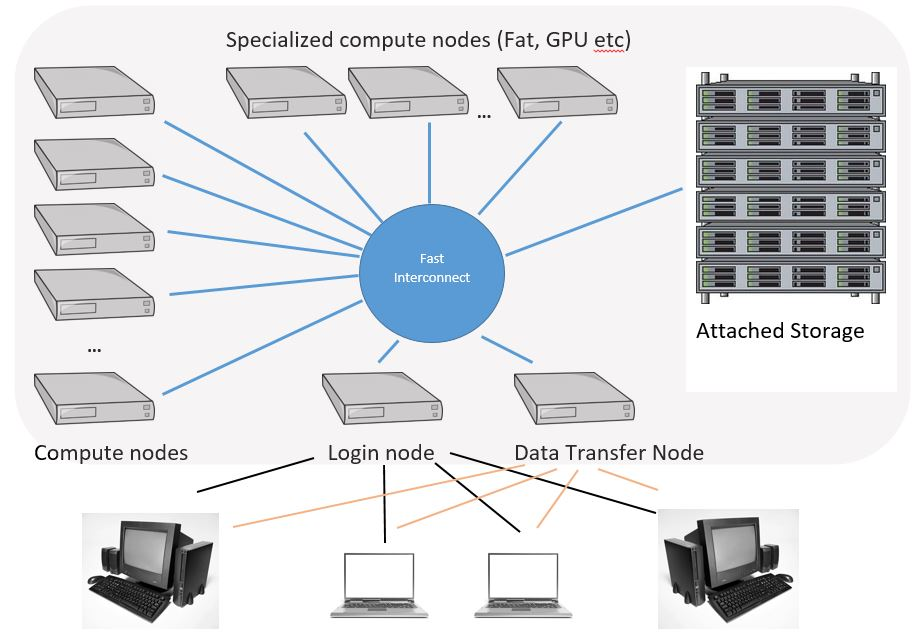
\includegraphics[height=2.70in,width=4.05in]{Figures/HPC_cluster.jpeg}
%\caption{\tiny \textrm{Pseudopotential for metallic sodium, based on the empty core model and screened by the Thomas-Fermi dielectric function.}}%(与文献\cite{EPJB33-47_2003}图1对比)
\label{HPC-Architecture-1}
\end{figure}
}

\frame
{
	\frametitle{高性能计算:~计算中心的资源分布}
\begin{figure}[h!]
\vspace*{-15pt}
\centering
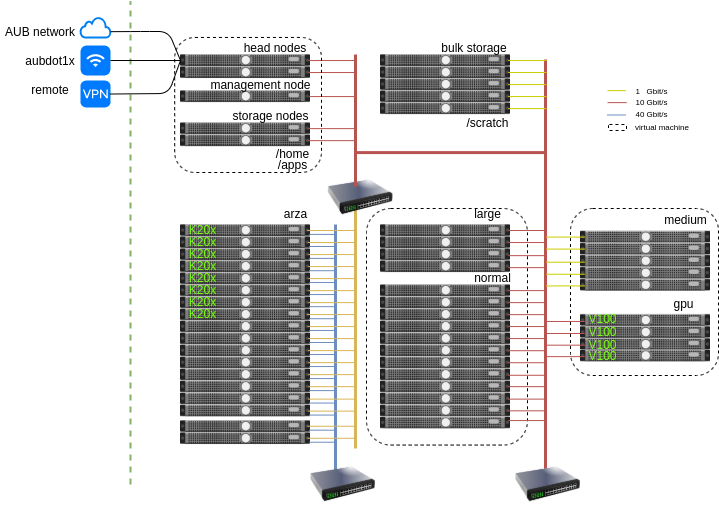
\includegraphics[height=2.40in,width=4.05in]{Figures/Architecture-of-HPC-Cluster_Octopus.png}
%\caption{\tiny \textrm{Pseudopotential for metallic sodium, based on the empty core model and screened by the Thomas-Fermi dielectric function.}}%(与文献\cite{EPJB33-47_2003}图1对比)
\label{Architecture-of-HPC-Cluster_Octopus}
\end{figure}
}

\frame
{
	\frametitle{计算中心:~多用户系统}
\begin{figure}[h!]
\vspace*{-10pt}
\centering
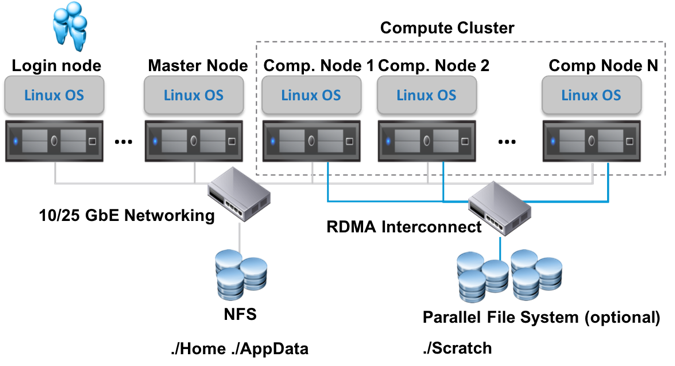
\includegraphics[height=2.30in,width=4.05in]{Figures/Traditional_bare-metal_HPC_cluster.png}
%\caption{\tiny \textrm{Pseudopotential for metallic sodium, based on the empty core model and screened by the Thomas-Fermi dielectric function.}}%(与文献\cite{EPJB33-47_2003}图1对比)
\label{HPC-Architecture-2}
\end{figure}
}

\frame
{
	\frametitle{高性能计算:~硬件}
\begin{figure}[h!]
\vspace*{-15pt}
\centering
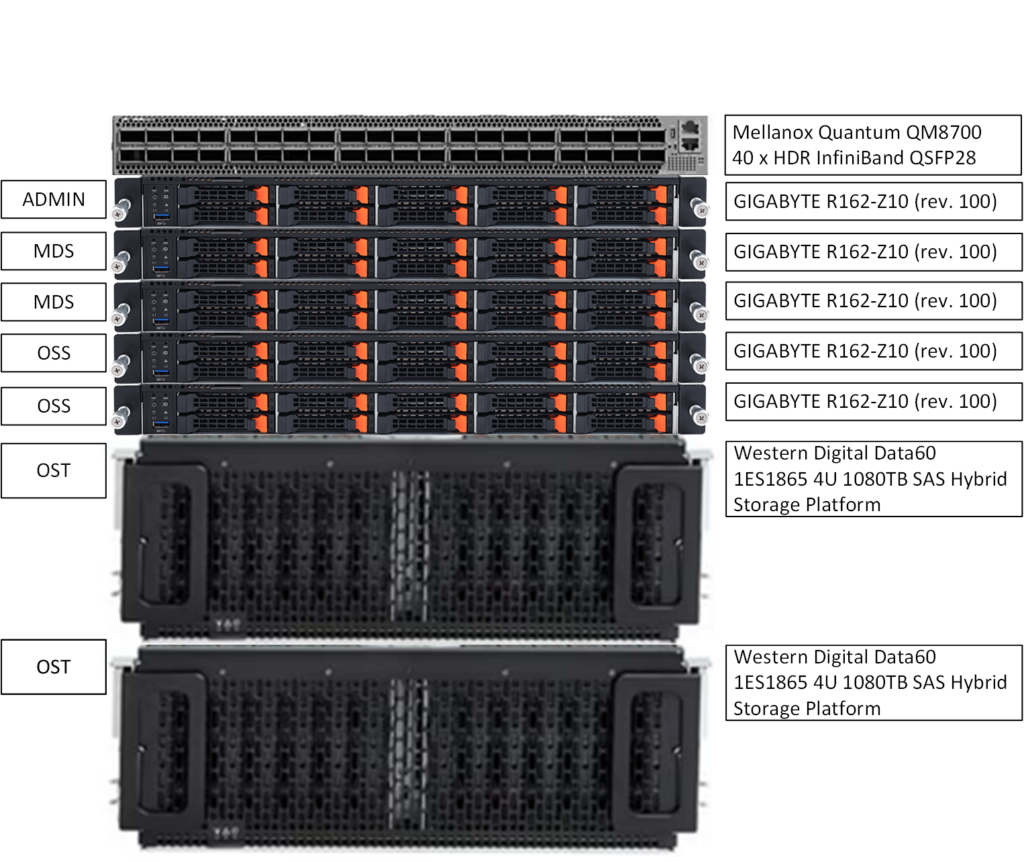
\includegraphics[height=2.80in,width=3.5in]{Figures/The_SDSU_petascale-parallel_storage_cluster-beekeeper.png}
%\caption{\tiny \textrm{Pseudopotential for metallic sodium, based on the empty core model and screened by the Thomas-Fermi dielectric function.}}%(与文献\cite{EPJB33-47_2003}图1对比)
\label{HPC-SDSU_petascale-parallel_storage_cluster-beekeeper}
\end{figure}
}

\frame
{
	\frametitle{高性能计算:~硬件}
\begin{figure}[h!]
\vspace*{-10pt}
\centering
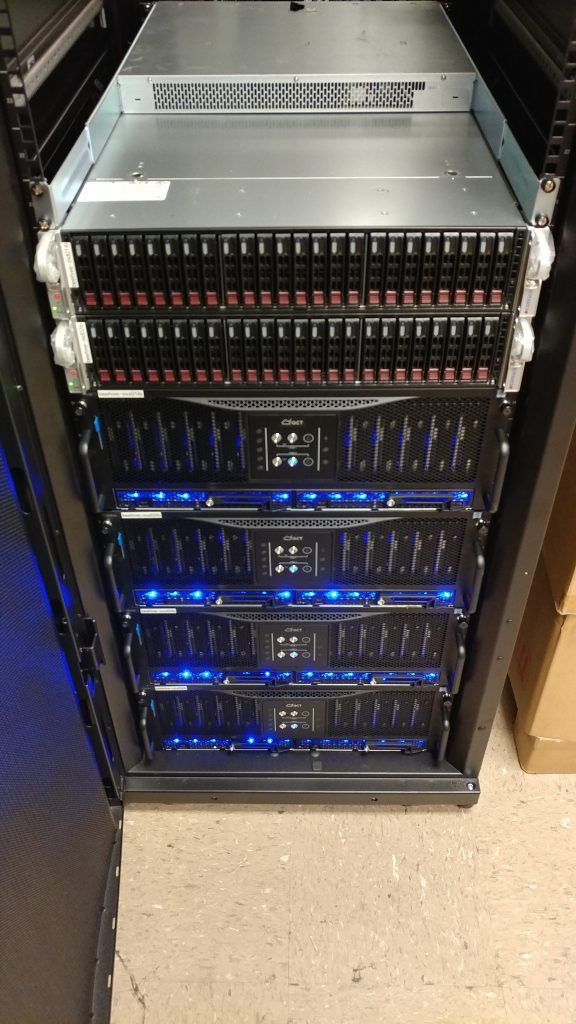
\includegraphics[height=2.80in,width=2.4in]{Figures/The_beehive_parallel_storage_cluster-in-the-Computational_Science_Data_Center.jpg}
%\caption{\tiny \textrm{Pseudopotential for metallic sodium, based on the empty core model and screened by the Thomas-Fermi dielectric function.}}%(与文献\cite{EPJB33-47_2003}图1对比)
\label{HPC-beehive_parallel_storage_cluster-in-the-Computational_Science_Data_Center}
\end{figure}
}

\frame
{
	\frametitle{高性能计算:~硬件}
\begin{figure}[h!]
\vspace*{-10pt}
\centering
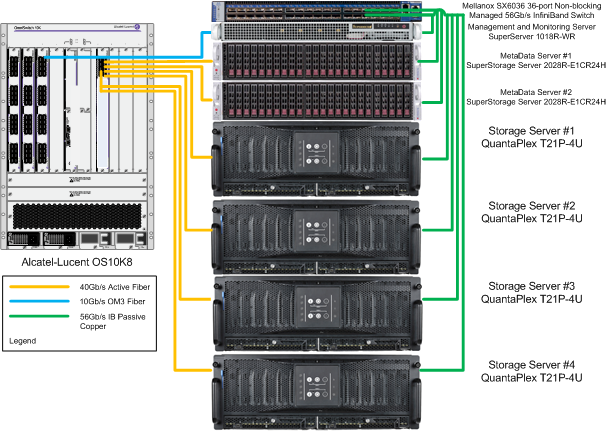
\includegraphics[height=2.80in,width=4.0in]{Figures/The_SDSU_petascale_parallel_storage_cluster_beehive.png}
%\caption{\tiny \textrm{Pseudopotential for metallic sodium, based on the empty core model and screened by the Thomas-Fermi dielectric function.}}%(与文献\cite{EPJB33-47_2003}图1对比)
\label{HPC-SDSU_petascale_parallel_storage_cluster_beehive}
\end{figure}
}

\frame
{
	\frametitle{高性能计算与高通量计算}
	\begin{itemize}
		\item \textrm{HPC~(High Performance Computing)}:
			\vskip 5pt
			\textrm{Large amounts of [simultaneous] computing power for comparatively short periods of time} 
		\item \textrm{HTC~(High Throughput Computing)}\footnote{\fontsize{5.5pt}{4.2pt}\selectfont{高通量的概念最初出现在实验领域,早期的材料研究、制药研究主要通过大量备选材料试错,最终才得到合适的材料或药物重要功能成分,这就是一种高通量筛选。文献中常会提到“高通量”和“组合方法”(\textrm{Combinational approach}),但很少区分两者的区别:~“高通量”指用户产生或处理的数据量极大,没有计算机自动处理无法完成;~而“组合方法”是针对影响研究对象的各种可能自由度的分门别类研究。换言之,高通量考虑的是利用计算机“一视同仁”地自动化式处理海量数据,而组合方法更强调对特定影响因素的筛查和组合研究}}:
			\vskip 5pt
			\textrm{Large amounts of computing over significantly longer periods, not necessarily all at the same time}
	\end{itemize}
}

\frame
{
	\frametitle{高性能计算与高通量计算}
\begin{figure}[h!]
%\vspace*{-0.05in}
\centering
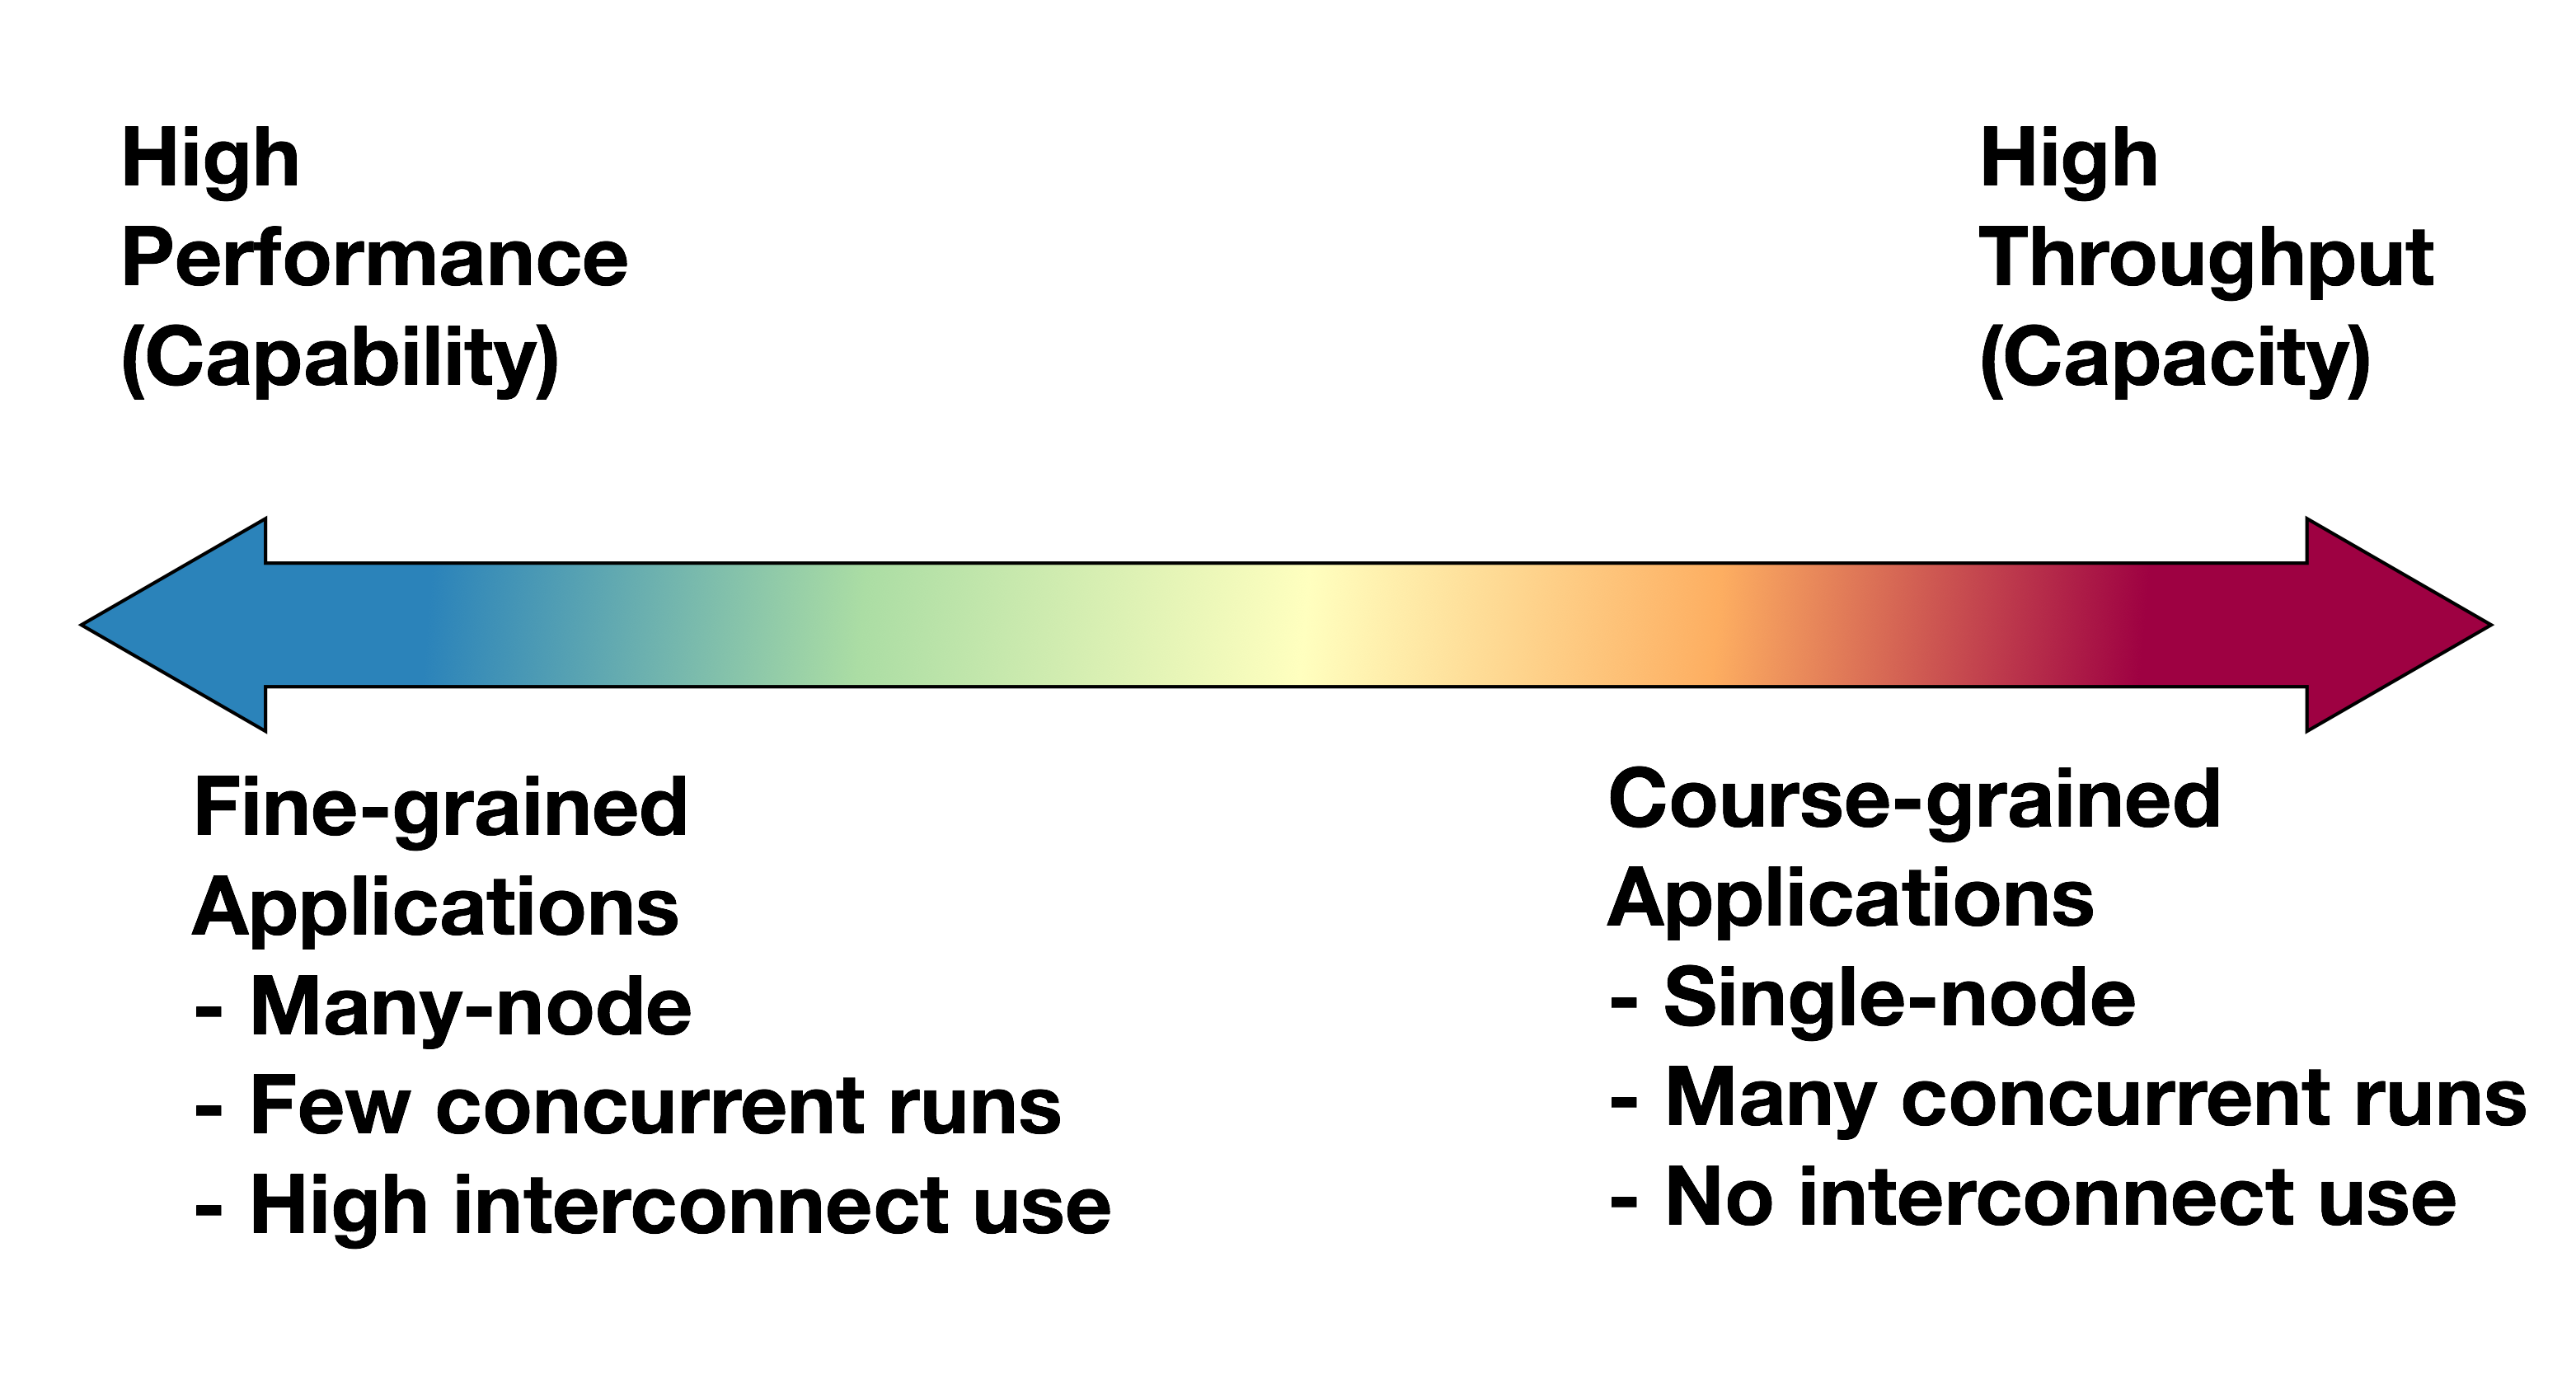
\includegraphics[height=2.30in,width=4.0in, viewport=0 0 765 367,clip]{HPC_vs_HTC.png}
%\caption{\tiny \textrm{Pseudopotential for metallic sodium, based on the empty core model and screened by the Thomas-Fermi dielectric function.}}%(与文献\cite{EPJB33-47_2003}图1对比)
\label{HPC_vs_HTC}
\end{figure}
}

\frame
{
	\frametitle{高性能计算与高通量计算}
	%\textrm{HTC}和\textrm{HPC}差异的一些特点。
	\textrm{HPC}和\textrm{HTC}作业可以在相同的集群架构上运行,但它们使用资源的方式不同:
			\vskip 8pt
	\begin{minipage}[t]{0.48\textwidth}
		{\fontsize{8.5pt}{5.2pt}\selectfont{\textrm{HPC}:~在需要时使用:}}
{\fontsize{6.5pt}{5.2pt}\selectfont{
	\begin{itemize}
		\item 运行需要中间结果快速通信以执行计算的作业
		\item 在相对较短的时间内大量使用计算资源
	\end{itemize}}}
\end{minipage}
\hfill
\begin{minipage}[t]{0.48\textwidth}
	{\fontsize{8.5pt}{5.2pt}\selectfont{\textrm{HTC}:~在需要时使用:}}
{\fontsize{6.5pt}{5.2pt}\selectfont{
	\begin{itemize}
		\item 运行许多通常相似但不高度并行的作业
		\item 使用不同的输入运行相同的程序
		\item 运行不相互通信的作业
		\item 利用使用网格启用技术的物理分布式资源
		\item 利用多个计算资源在较长时间内执行计算任务
	\end{itemize}}}
\end{minipage}
			\vskip 8pt
	\begin{itemize}
		\item {\fontsize{8.5pt}{5.2pt}\selectfont{\textrm{HPC}作业通常涉及在许多处理器上运行并行软件的单个实例}}
			\vskip 1pt
			{\fontsize{6.5pt}{5.2pt}\selectfont{在计算的各个实例中,结果在处理器之间进行通信,需要并行环境}}
		\item {\fontsize{8.5pt}{5.2pt}\selectfont{\textrm{HTC}作业通常涉及在多个处理器上同时运行软件的多个独立实例}}
			\vskip 1pt
			{\fontsize{6.5pt}{5.2pt}\selectfont{串行系统适用于这些要求}}
	\end{itemize}
}

\frame
{
	\frametitle{高性能计算与高通量计算}
\begin{figure}[h!]
\vspace*{-10pt}
\centering
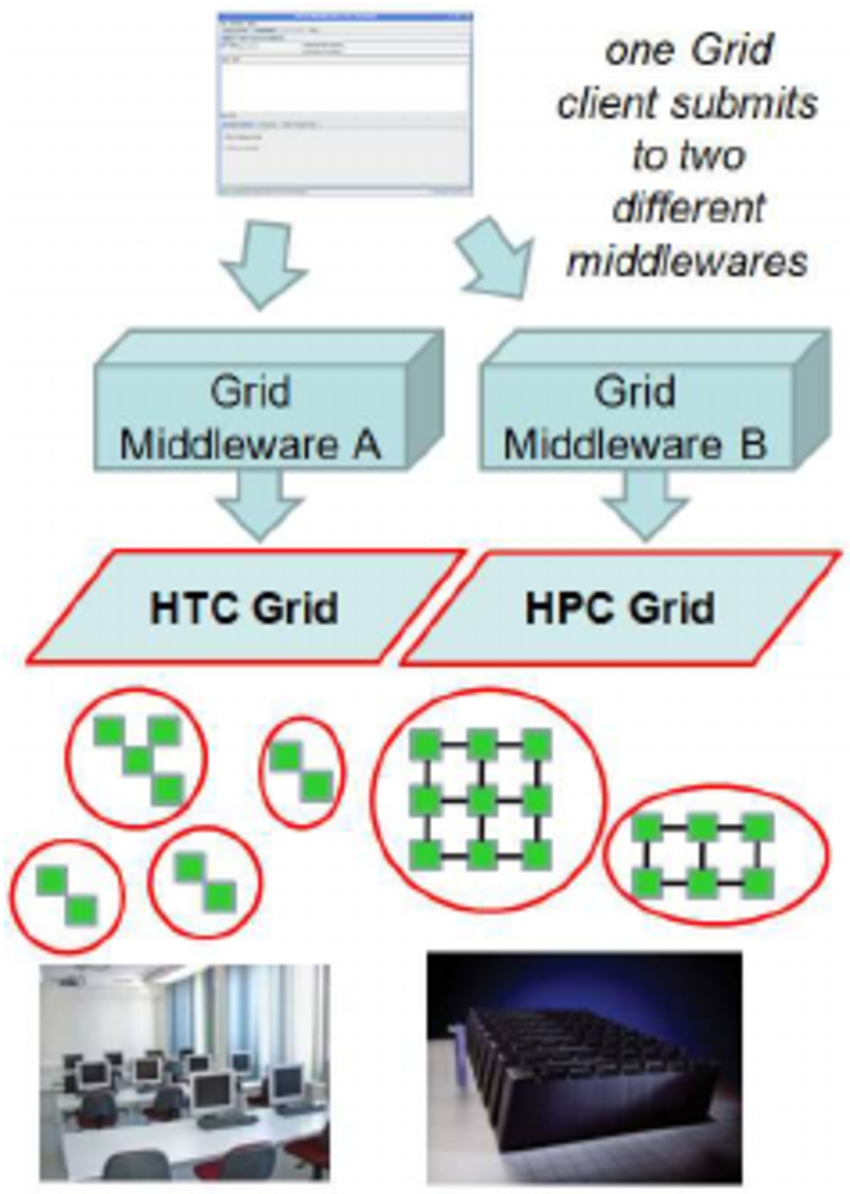
\includegraphics[height=2.80in,width=2.2in]{Figures/Interoperability-of-HTC-and-HPC-infrastructures-enables-new-types-of-e-science.png}
%\caption{\tiny \textrm{Pseudopotential for metallic sodium, based on the empty core model and screened by the Thomas-Fermi dielectric function.}}%(与文献\cite{EPJB33-47_2003}图1对比)
\label{Interoperability-of-HTC-and-HPC-infrastructures-enables-new-types-of-e-science}
\end{figure}
}

\frame
{
	\frametitle{复杂计算流程:~高性能与高通量}
\begin{figure}[h!]
\vspace*{-10pt}
\centering
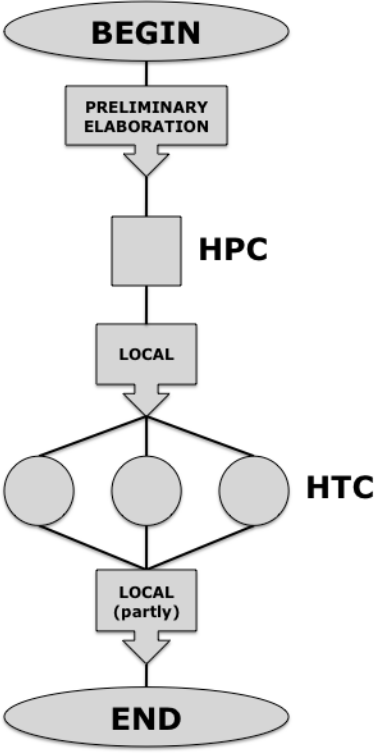
\includegraphics[height=2.80in,width=1.6in]{Figures/The_combined_GriF_HPC-HTC_Workflow.png}
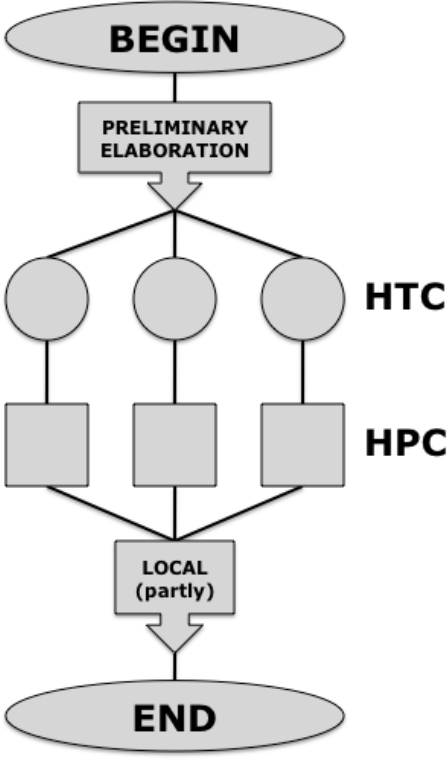
\includegraphics[height=2.80in,width=1.7in]{Figures/The_combined_GriF_HTC-HPC_Workflow.png}
%\caption{\tiny \textrm{Pseudopotential for metallic sodium, based on the empty core model and screened by the Thomas-Fermi dielectric function.}}%(与文献\cite{EPJB33-47_2003}图1对比)
\label{The_combined-HTC-HPC_Workflow}
\end{figure}
}

%\frame
%{
%	\frametitle{\textrm{High Performance vs High Throughput}}
%\begin{minipage}{0.47\textwidth}
%	\textbf{HPC}
%	\begin{itemize}
%		\item \textrm{Focus:\,Large workflows of \underline{\textcolor{blue}{highly-interdependent}} sub-tasks}
%		\item \textrm{More~important:\,persistent access to the fastest cores, CPU homogenity, special coding, shared filesystems, fast networks}
%	\end{itemize}
%\end{minipage}
%\hskip 2pt
%\begin{minipage}{0.47\textwidth}
%	\textbf{HTC}
%	\begin{itemize}
%		\item \textrm{Focus:\,Large workflows of \textcolor{blue}{\underline{numerous},\underline{relatively small},}and \textcolor{blue}{\underline{independent}} compute tasks}
%		\item \textrm{More~important:\,maximized number of running tasks}
%		\item \textrm{Less~important:~ CPU speed, homogeneity}
%	\end{itemize}
%\end{minipage}
%}
%
%\frame
%{
%	\frametitle{高性能计算与高通量计算}
%\begin{table}[!h]
%\tabcolsep 0pt \vspace*{-12pt}
%%\caption{}
%\label{Table-Cost}
%\begin{minipage}{1.00\textwidth}
%%\begin{center}
%\centering
%\def\temptablewidth{1.0\textwidth}
%\renewcommand\arraystretch{0.8} %表格宽度控制(普通表格宽度的两倍)
%%\rule{\temptablewidth}{1pt}
%\begin{tabular*} {\temptablewidth}{@{\extracolsep{\fill}}c@{\extracolsep{\fill}}c@{\extracolsep{\fill}}c}
%	\toprule[2pt]        %% 绘制三线表顶端线,粗细设置
%%-------------------------------------------------------------------------------------------------------------------------
%	{\fontsize{5.5pt}{5.2pt}\selectfont{\textrm{Parameter}}}&{\fontsize{5.0pt}{5.2pt}\selectfont{高性能计算\textrm{(HPC)}}}	&{\fontsize{5.0pt}{5.2pt}\selectfont{高通量计算\textrm{(HTC)}}}\\%\hline
%	\midrule[1pt]        %% 绘制三线表中间线,粗细设置
%%	\raisebox{-1ex}[0pt][0pt]{\fontsize{5.5pt}{5.2pt}\selectfont{\textrm{Stands for}}} &{\fontsize{5.5pt}{5.2pt}\selectfont{\textrm{HPC stands for}}} &{\fontsize{5.5pt}{5.2pt}\selectfont{\textrm{HTC stands for}}}\\
%%	 &{\fontsize{5.5pt}{5.2pt}\selectfont{\textrm{High-Performance Computing}}} & {\fontsize{5.5pt}{5.2pt}\selectfont{\textrm{High-Throughput Computing}}}\\\hline
%	 &{\fontsize{4.0pt}{5.2pt}\selectfont{\textrm{HPC is defined as the type of computing that}}} &{\fontsize{4.0pt}{5.2pt}\selectfont{\textrm{HTC is defined as a type of computing that}}}\\
%	 {\fontsize{7.0pt}{5.2pt}\selectfont{\textrm{Definition}}} &{\fontsize{4.0pt}{5.2pt}\selectfont{\textrm{makes use of multiple computer processors in order}}} &{\fontsize{4.0pt}{5.2pt}\selectfont{\textrm{parallelly executes a large number of}}} \\
%&{\fontsize{4.0pt}{5.2pt}\selectfont{\textrm{to perform complex computations parallelly.}}} &{\fontsize{4.0pt}{5.2pt}\selectfont{\textrm{simple and computationally independent tasks.}}}\\\hline
%&{\fontsize{4.0pt}{5.2pt}\selectfont{\textrm{HPC consists of running large-scale, complex,}}} &{\fontsize{4.0pt}{5.2pt}\selectfont{\textrm{HTC consists of running a large number of tasks}}}\\
%{\fontsize{5.5pt}{5.2pt}\selectfont{\textrm{Workload}}} &{\fontsize{4.0pt}{5.2pt}\selectfont{\textrm{and computationally intensive applications that}}} &{\fontsize{4.0pt}{5.2pt}\selectfont{\textrm{ that are independent and small in size and does}}}\\
%&{\fontsize{4.0pt}{5.2pt}\selectfont{\textrm{need significant resources and memory.}}} &{\fontsize{4.0pt}{5.2pt}\selectfont{\textrm{not require a large amount of memory and resources.}}}\\\hline
% \raisebox{-1ex}[0pt][0pt]{\fontsize{6.0pt}{5.2pt}\selectfont{\textrm{Processing}}}&{\fontsize{4.0pt}{5.2pt}\selectfont{\textrm{HPC is designed to provide maximum}}} &{\fontsize{4.0pt}{5.2pt}\selectfont{\textrm{HTC is designed to increase the number}}}\\
% \raisebox{-1ex}[0pt][0pt]{\fontsize{6.0pt}{5.2pt}\selectfont{\textrm{Power}}}&{\fontsize{4.0pt}{5.2pt}\selectfont{\textrm{ performance and speed for large tasks.}}} &{\fontsize{4.0pt}{5.2pt}\selectfont{\textrm{of tasks that needs to be completed in a given}}}\\
%& &{\fontsize{4.0pt}{5.2pt}\selectfont{\textrm{specific amount of time.}}}\\\hline
% \raisebox{-1ex}[0pt][0pt]{\fontsize{6.0pt}{5.2pt}\selectfont{\textrm{Resource}}} &{\fontsize{4.0pt}{5.2pt}\selectfont{\textrm{For resource management to processes,}}}&{\fontsize{4.0pt}{5.2pt}\selectfont{\textrm{For the resource management to processes,}}}\\
% \raisebox{-1ex}[0pt][0pt]{\fontsize{6.0pt}{5.2pt}\selectfont{\textrm{Management}}}&{\fontsize{4.0pt}{5.2pt}\selectfont{\textrm{HPC makes use of job schedulers and}}} &{\fontsize{4.0pt}{5.2pt}\selectfont{\textrm{HTC makes use of distributed management}}}\\
% &{\fontsize{4.0pt}{5.2pt}\selectfont{\textrm{ resource managers.}}} &{\fontsize{4.0pt}{5.2pt}\selectfont{\textrm{resources.}}}\\\hline
% \raisebox{-1ex}[0pt][0pt]{\fontsize{6.0pt}{5.2pt}\selectfont{\textrm{Fault}}}&{\fontsize{4.0pt}{5.2pt}\selectfont{\textrm{To reduce the risk of data loss and}}}&{\fontsize{4.0pt}{5.2pt}\selectfont{\textrm{HTC systems do not affect any}}}\\
% \raisebox{-1ex}[0pt][0pt]{\fontsize{6.0pt}{5.2pt}\selectfont{\textrm{Tolerance}}}&{\fontsize{4.0pt}{5.2pt}\selectfont{\textrm{data corruption HPC systems have a}}} &{\fontsize{4.0pt}{5.2pt}\selectfont{\textrm{other running processes due to the}}}\\
%&{\fontsize{4.0pt}{5.2pt}\selectfont{\textrm{complex fault tolerance mechanism.}}} &{\fontsize{4.0pt}{5.2pt}\selectfont{\textrm{failure of an individual task.}}}\\\hline
% &{\fontsize{4.0pt}{5.2pt}\selectfont{\textrm{HPC scales up when few}}} &{\fontsize{4.0pt}{5.2pt}\selectfont{\textrm{HTC systems scale horizontally for}}}\\
% {\fontsize{6.0pt}{5.2pt}\selectfont{\textrm{Scaling}}} &{\fontsize{4.0pt}{5.2pt}\selectfont{\textrm{users are running together.}}} &{\fontsize{4.0pt}{5.2pt}\selectfont{\textrm{simple tasks and require less}}}\\
% & &{\fontsize{4.0pt}{5.2pt}\selectfont{\textrm{computational speed.}}}\\\hline
% &{\fontsize{4.0pt}{5.2pt}\selectfont{\textrm{HPC can be used in applications such as}}}&{\fontsize{4.0pt}{5.2pt}\selectfont{\textrm{HTC can be used in applications such as}}}\\
% {\fontsize{6.0pt}{5.2pt}\selectfont{\textrm{Applications}}} &{\fontsize{4.0pt}{5.2pt}\selectfont{\textrm{engineering design, weather forecasting,}}}&{\fontsize{4.0pt}{5.2pt}\selectfont{\textrm{bioinformatics, research applications,}}}\\
% &{\fontsize{4.0pt}{5.2pt}\selectfont{\textrm{drug discovery etc.}}} &{\fontsize{4.0pt}{5.2pt}\selectfont{\textrm{etc.}}}\\%\hline
%	\bottomrule[1.8pt]     %%绘制三线表底部线,粗细设置
%\end{tabular*}
%%\rule{\temptablewidth}{1pt}
%\end{minipage}
%%\vskip -15pt
%%\end{center}
%\end{table}
%}
%
\frame
{
	\frametitle{科学研究的范式变更}
\begin{figure}[h!]
\vspace*{0.08in}
\centering
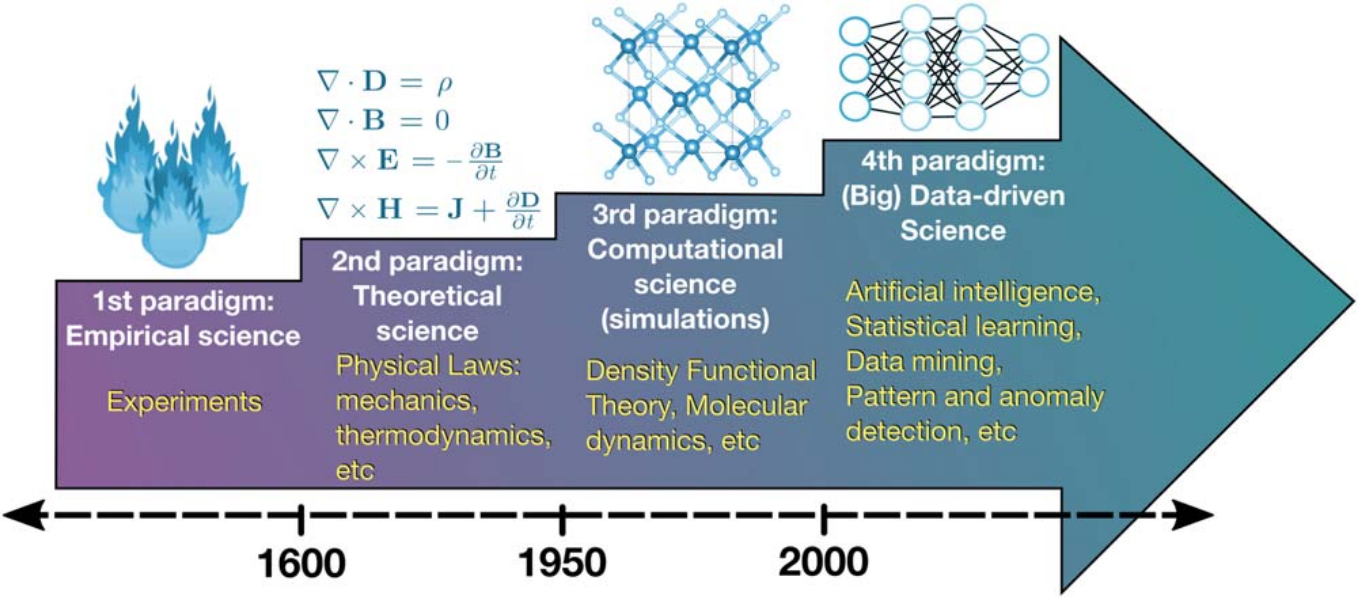
\includegraphics[height=2.00in,width=4.15in]{Figures/Four_Model_3.png}
%\caption{\tiny \textrm{Pseudopotential for metallic sodium, based on the empty core model and screened by the Thomas-Fermi dielectric function.}}%(与文献\cite{EPJB33-47_2003}图1对比)
\label{Four_Model}
\end{figure}
}

\frame
{
	\frametitle{数据驱动的科学研究}
前所未有的计算能力和大规模的数据收集能力%,现代科学正在进入“第四范式”:
\begin{figure}[h!]
%\vspace*{-0.05in}
\centering
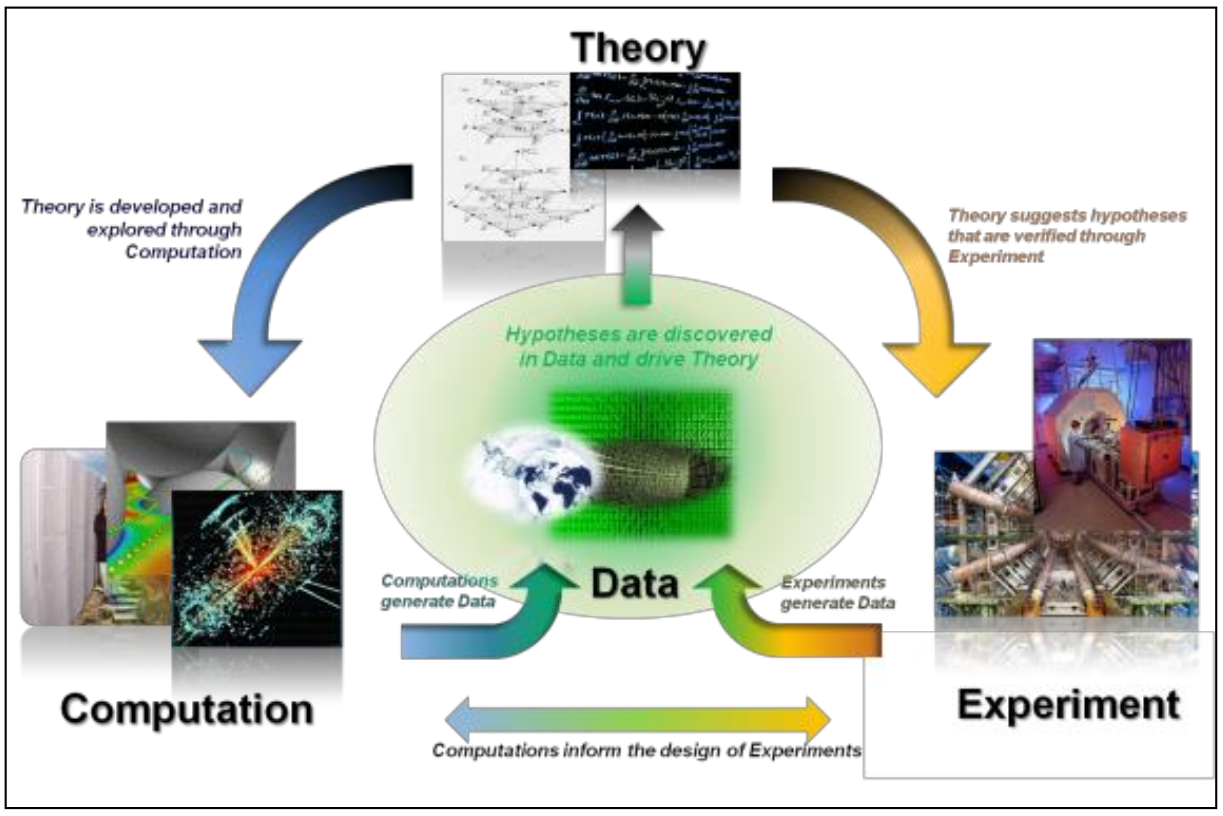
\includegraphics[height=2.40in,width=3.75in]{Figures/Four_Model_1.png}
%\caption{\tiny \textrm{Pseudopotential for metallic sodium, based on the empty core model and screened by the Thomas-Fermi dielectric function.}}%(与文献\cite{EPJB33-47_2003}图1对比)
\label{Four_Model_1}
\end{figure}
科学的新驱动力:~\textcolor{red}{密集数据}+\textcolor{red}{人工智能}
}

\section{高通量计算材料自动流程}
\frame
{
	\frametitle{高通量计算流程}
高通量计算流程主要任务包括三方面:
\begin{itemize}
	\item \textcolor{blue}{增加材料模拟数据}:~主要包括\textrm{DFT}、\textrm{MD}计算的材料数据
	\item \textcolor{blue}{存储材料物性数据}:~系统存储材料数据,用以构建材料数据库
		\vskip 2pt
		{\fontsize{6.5pt}{4.2pt}\selectfont{材料数据库包括通用材料数据库或特定目标的材料数据库}}
\item \textcolor{blue}{检索材料数据}:~对存储的材料数据实施检索和分析,服务材料性能提升需求
\end{itemize}
高通量计算流程的主要目标之一就是构建材料数据库
\vskip 2pt
{\fontsize{7.5pt}{4.2pt}\selectfont{\textcolor{cyan}{高通量计算流程与数据密不可分:~著名的高通量计算流程都有相应的数据库}
\begin{itemize}
	\item \textrm{AFLOW}的数据库为\textrm{AFLOWLIB}
	\item \textrm{MP}的数据库为同名的\textrm{Materials Project}
	\item \textrm{ASE}的数据库为\textrm{CMR~(The Computational Materials Repository)}
\end{itemize}
%,,。中科院物理所也拥有一个通用的材料科学数据库\textrm{Atomly}
}}
}

\frame
{
	\frametitle{国外已有的计算平台}
\begin{figure}[h!]
\centering
\vspace{-15.5pt}
\subfigure[\fontsize{6.5pt}{6.2pt}\selectfont{\textrm{Auto-FLOW (AFLOW)}\upcite{CMS58-227_2012}}]{
\label{AFLOW_data_flow}
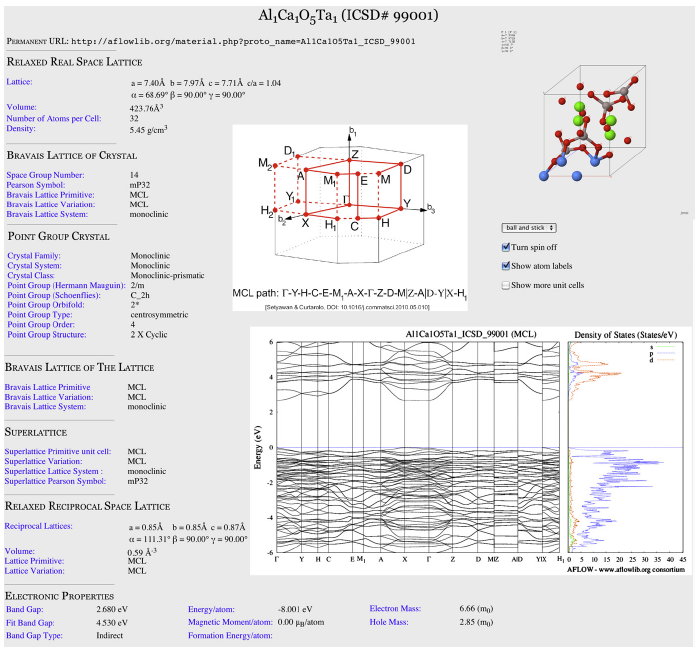
\includegraphics[height=1.2in,width=1.6in,viewport=0 0 720 660,clip]{Figures/AFLOW_database.png}}
\subfigure[\fontsize{6.5pt}{6.2pt}\selectfont{\textrm{Material Project (MP)}\upcite{CMS97-209_2015}}]{
\label{MP_commp_infrastructure}
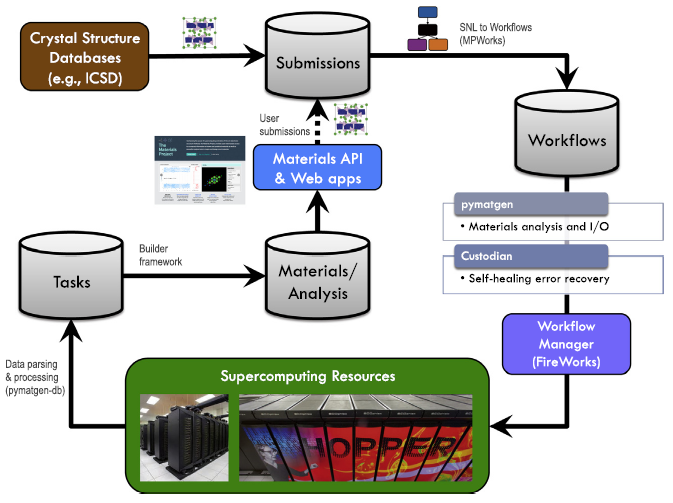
\includegraphics[height=1.2in,width=1.7in,viewport=0 0 670 530,clip]{Figures/MP_comp_infrastructure.png}}
\subfigure[\fontsize{3.5pt}{3.2pt}\selectfont{\textrm{Quantum Materials Informatics Project (QMIP)}\upcite{url_QMIP}}]{
\label{QMIP_Shame}
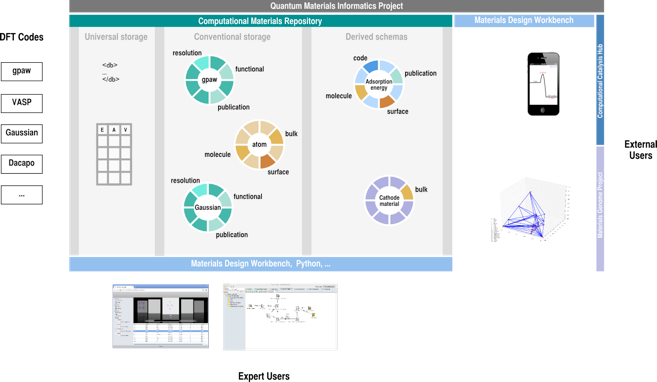
\includegraphics[height=1.2in,width=1.7in,viewport=0 0 670 420,clip]{Figures/QMIP_shame.png}}
\subfigure[\fontsize{6.5pt}{5.2pt}\selectfont{\textrm{Clean Energy Project (CEP)}\upcite{JPCL2-2241_2011}}]{
\label{CEP_structure_flow}
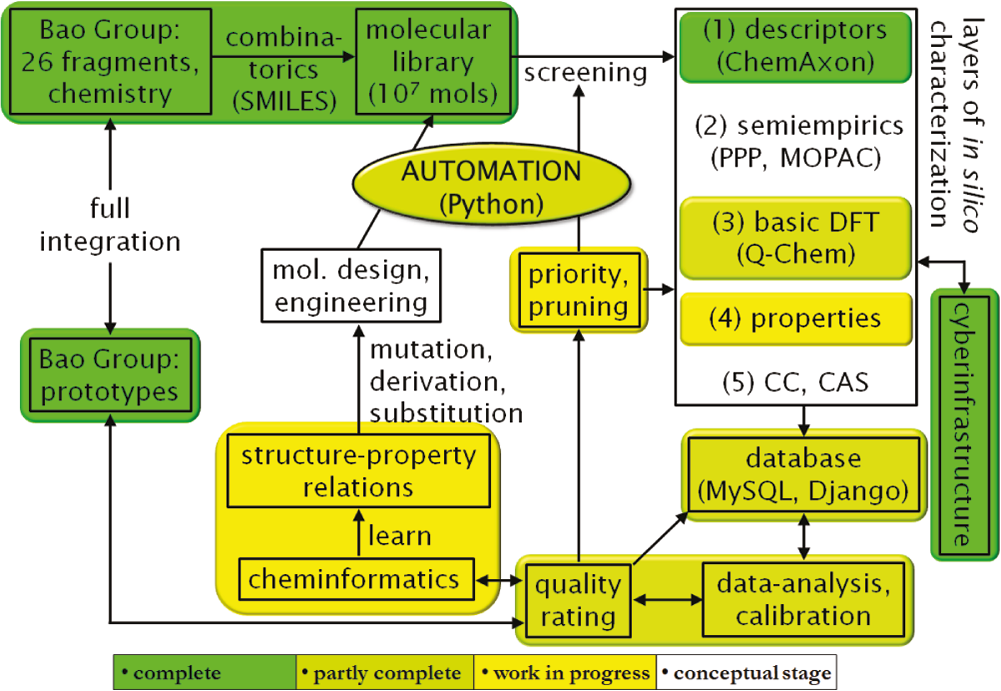
\includegraphics[height=1.2in,width=1.6in,viewport=0 0 1020 730,clip]{Figures/CEP_structure_flow.png}}
%\caption{}%
\label{Auto_Flow_Platform-1}
\end{figure}
}

\frame
{
	\frametitle{国内已有的计算平台:~\textrm{MatCloud}}
\begin{figure}[h!]:
\centering
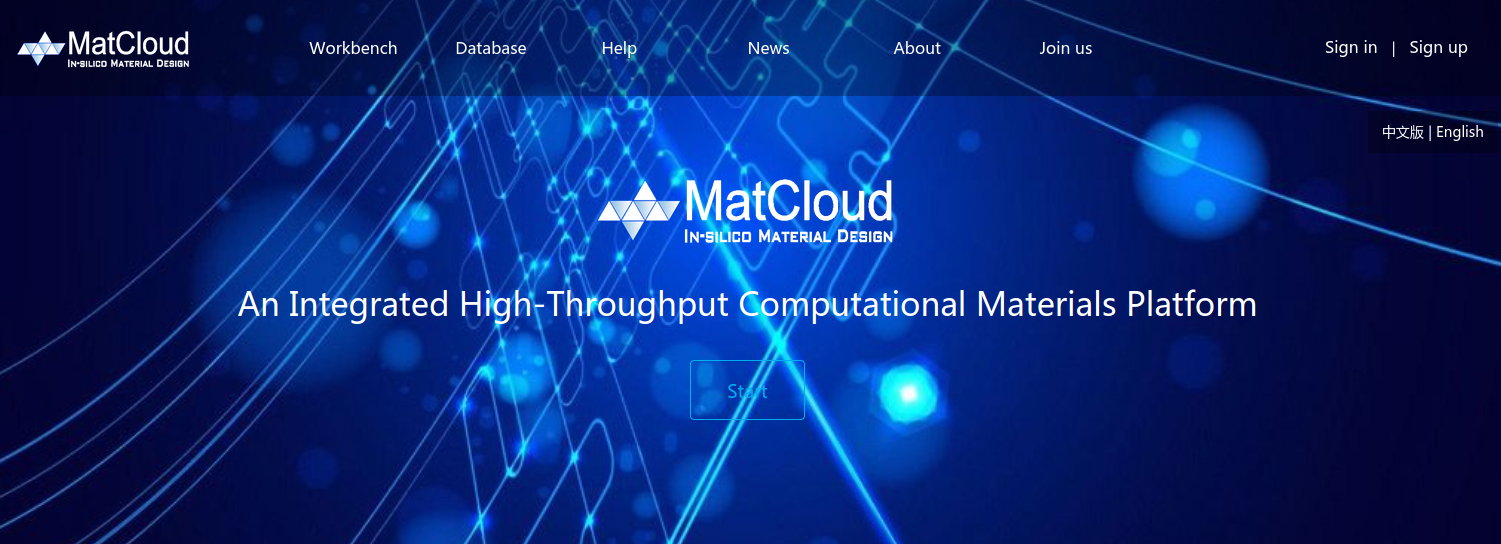
\includegraphics[height=1.57in,width=4.95in,viewport=0 0 1800 550,clip]{Figures/Matcloud-login.png}
\caption{\fontsize{7.2pt}{4.2pt}\selectfont{中科院计算机网络信息中心~杨小渝团队开发}\upcite{CMS146-319_2018,url_Matcloud}}%
\label{Auto_Flow_Platform-2}
\end{figure}
}

\frame
{
	\frametitle{高通量计算自动流程} 
当前高通量计算的自动处理流程集中在材料模拟的计算数据收集和实现计算结果自动入库为主
\vskip 2pt
{\fontsize{7.5pt}{4.2pt}\selectfont{材料第一原理计算的软件有很多,输出文件的格式千差万别,通过第一原理计算构建相对完善的材料数据库需要耗费相当的计算资源和人力}}
\vskip 5pt
自动流程面向的对象是数据,要实现材料计算过程的自动处理,首先需要解决的是数据格式的规范化
\begin{itemize}
	\item \textcolor{magenta}{数据规范化类型}:~面向各类软件输出数据的自动化提取与传输
\vskip 2pt
{\fontsize{6.5pt}{4.2pt}\selectfont{根据软件的计算特点,组织多种软件实现材料物性计算:~\textcolor{blue}{灵活性较好,但一般只支持相对简单的计算流程}}}
\item \textcolor{magenta}{流程规范化类型}:~面向材料计算软件的标准化流程,通过数据库支持 
\vskip 2pt
{\fontsize{6.5pt}{4.2pt}\selectfont{利用数据库技术将自动流程组织得更复杂多样,并作为数据库条目存储下来:~\textcolor{blue}{稳定性较好,但计算的材料物性受软件能力的限制较多}}}
\end{itemize}
\textcolor{purple}{主要的自动流程采用\textrm{Python}语言实现}:~跨平台、模块化组织灵活
}

\frame
{
	\frametitle{计算平台的功能和总体架构}
\begin{figure}[h!]
\centering
\vspace*{-0.35in}
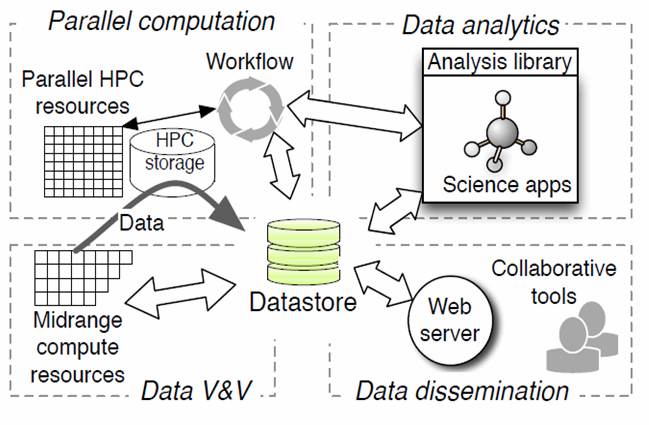
\includegraphics[height=2.6in,width=4.05in,viewport=0 0 670 460,clip]{Figures/Parallel_computation.png}
%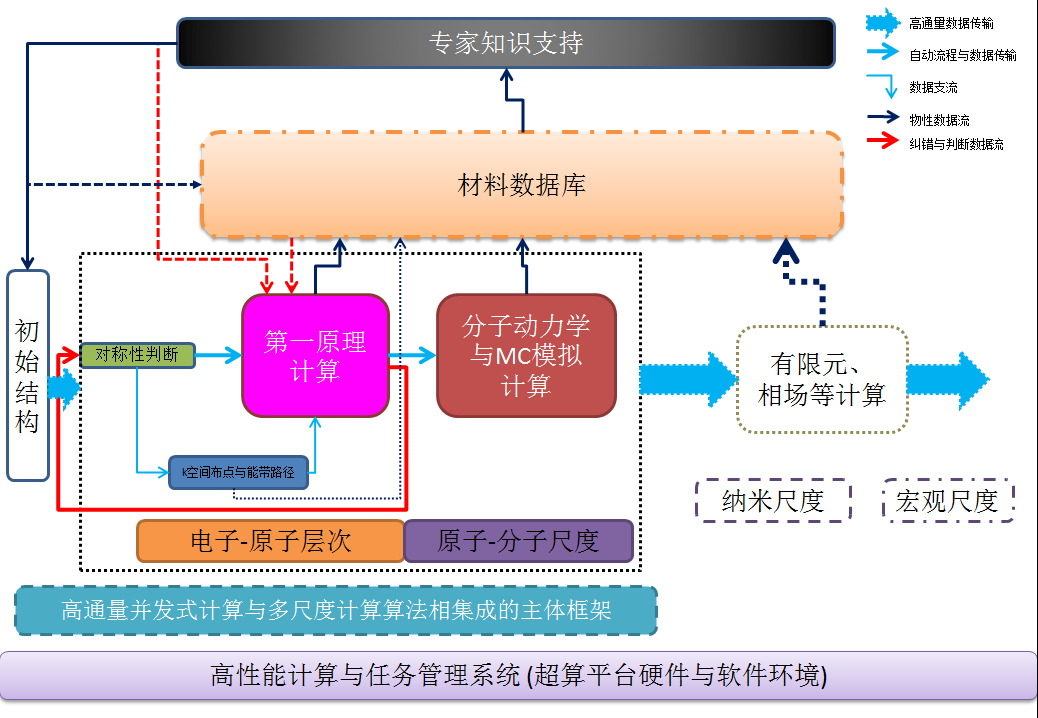
\includegraphics[height=1.6in,width=2.4in,viewport=0 0 1038 730,clip]{Figures/Auto_Flow.png}
\caption{\fontsize{7.2pt}{4.2pt}\selectfont{\textrm{The schematic framework and platform of all those project.}}}%
\label{Auto_Flow}
\end{figure} 
}

\frame
{
	\frametitle{材料计算软件发展现状}
\begin{figure}[h!]
\vspace*{-0.16in}
\centering
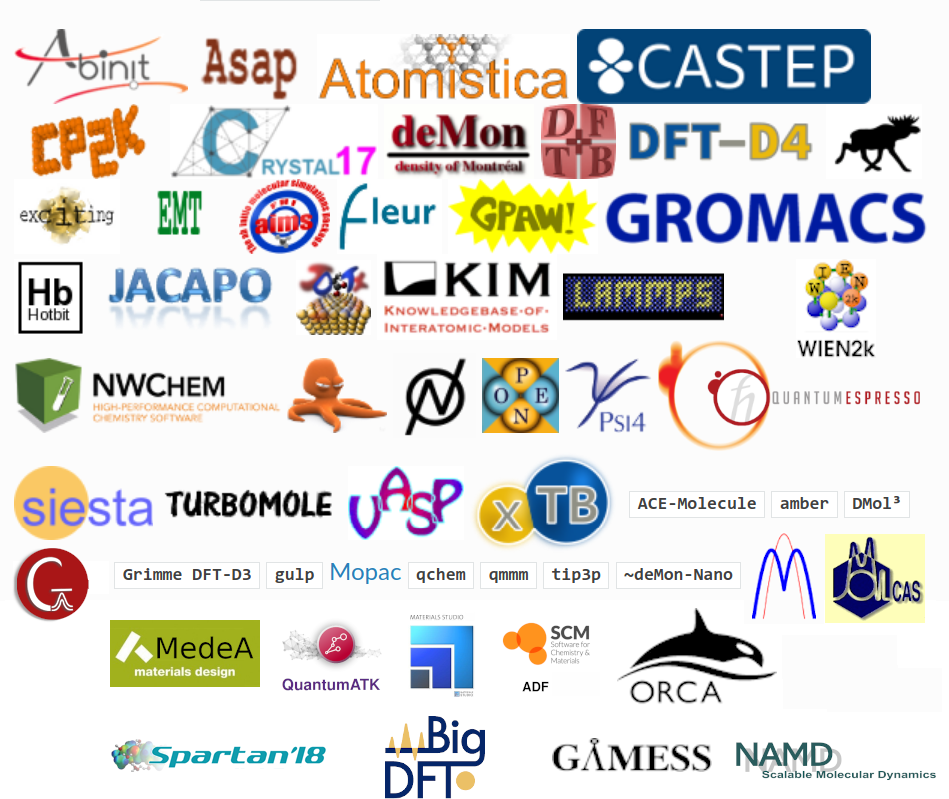
\includegraphics[width=3.30in]{Figures/Softwares_logo.png}
%\caption{\tiny \textrm{Pseudopotential for metallic sodium, based on the empty core model and screened by the Thomas-Fermi dielectric function.}}%(与文献\cite{EPJB33-47_2003}图1对比)
\label{Softwares}
\end{figure}
}

\frame
{
	\frametitle{国产第一原理计算软件现状}
\begin{figure}[h!]
\vspace*{-0.19in}
\centering
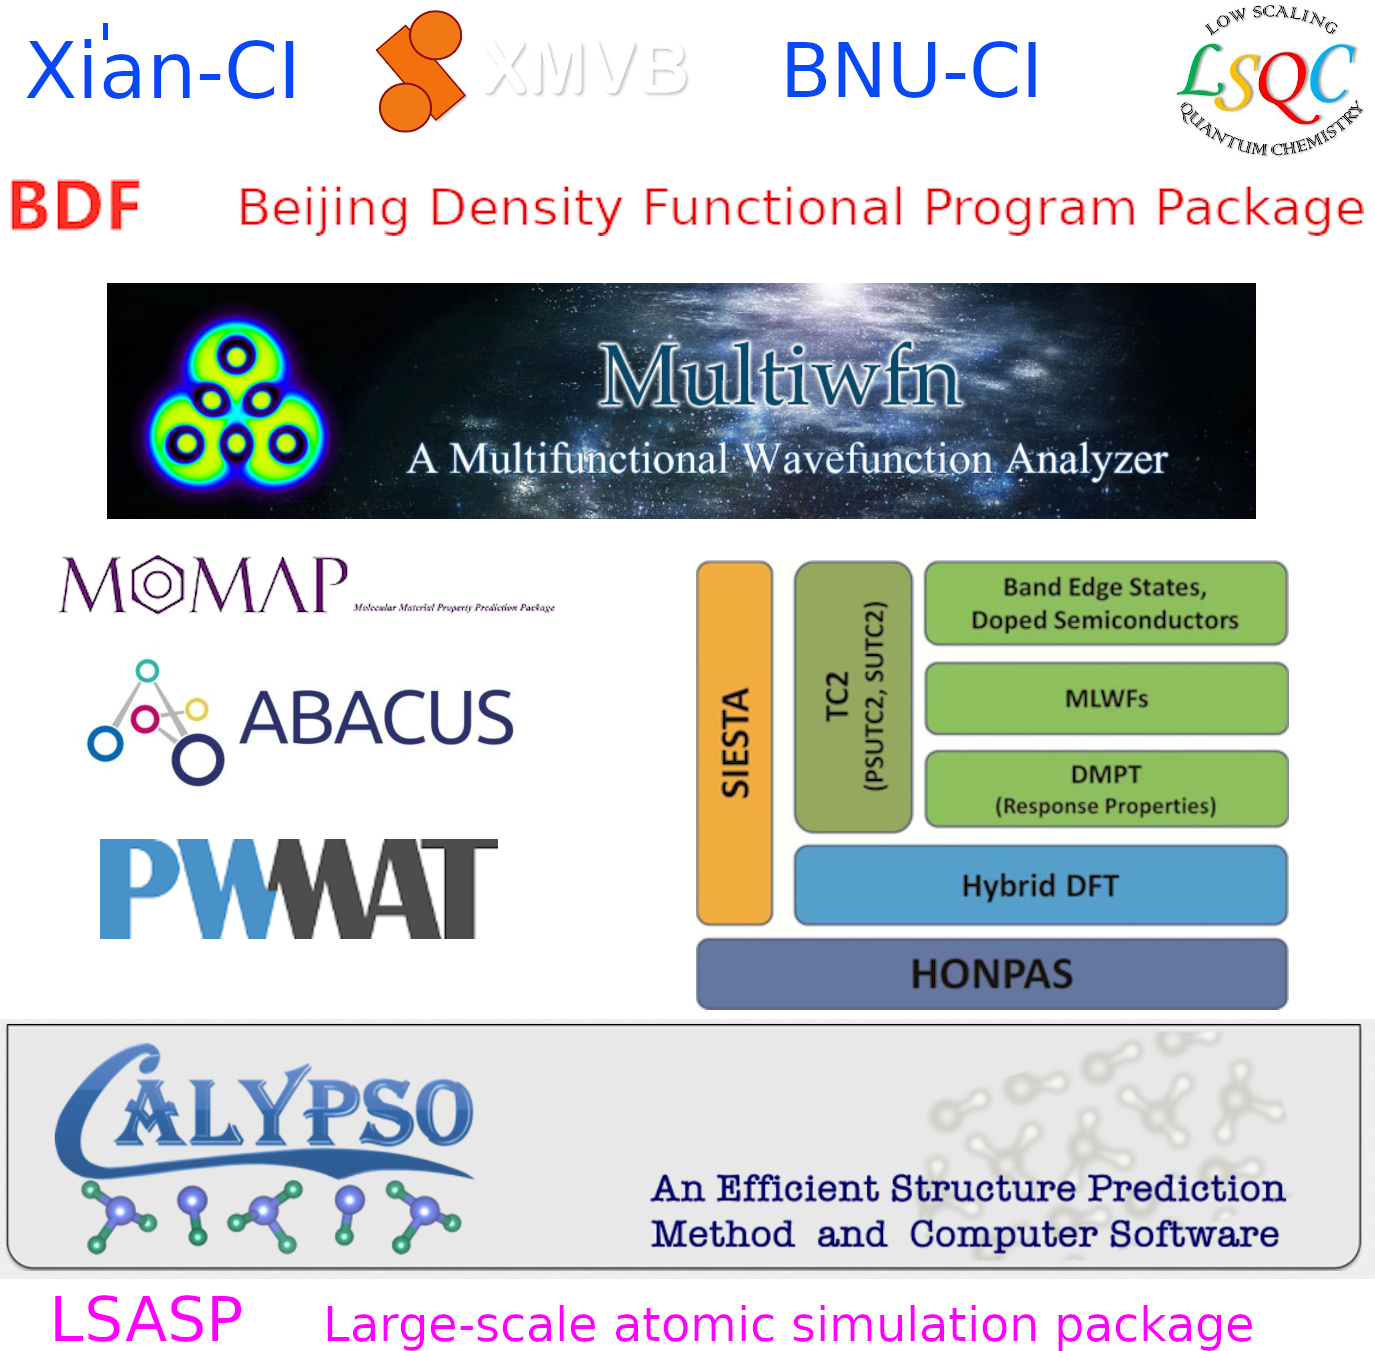
\includegraphics[width=2.83in]{Figures/Softwares_China-logo.png}
%\caption{\tiny \textrm{Pseudopotential for metallic sodium, based on the empty core model and screened by the Thomas-Fermi dielectric function.}}%(与文献\cite{EPJB33-47_2003}图1对比)
\label{Software-China}
\end{figure}
	\fontsize{6.2pt}{5.2pt}\selectfont{\textcolor{red}{中国学科发展战略\,$\cdot$\,理论与计算化学,~~国家自然科学基金委员会,~中国科学院,~~北京:~科学出版社,~~2016}}
}

\frame
{
	\frametitle{\textrm{ASE}自动流程的设计与管理}
数据规范化型的自动处理以\textrm{ASE}为典型代表,通过各类\textrm{Python}模块,支持多种\textrm{DFT-MD}软件%。根据图\ref{Auto_Flow_Platform-5}可知,\textrm{ASE}的核心模块主要包括\textrm{Atoms}(原子、分子建模)、\textrm{Calculator}(各类计算软件运行支持与控制)和物性计算、功能分析和结果可视化模块。
\vskip 3pt
		\textcolor{purple}{\textrm{ASE}特色}:~模块加载式计算流程控制,符合复杂多尺度计算场景
		\begin{itemize}
			\item \textcolor{magenta}{灵活的建模功能}
				\begin{enumerate}
    \setlength{\itemsep}{7pt}
					\item 简单组织:~原子直接构成分子
					\item 理想周期体系(包括一维、二维、三维)
					\item 表面和表面吸附,可指定吸附位
				\end{enumerate}
			\item \textcolor{magenta}{丰富的软件接口}\\
				提供了包括绝大部分第一原理和分子动力学计算软件接口,方便组合实现多尺度计算
			\item \textcolor{magenta}{不依赖软件的优化与动力学模拟}\\
				适合复杂材料物性模拟的优化和多种动力学过程模拟
			\item \textcolor{magenta}{多样化的数据库类型}
		\end{itemize} 
}

\frame
{
\frametitle{\textrm{ASE}的结构生成模块}
\begin{minipage}[b]{0.48\textwidth}
	{\fontsize{7.8pt}{5.2pt}\selectfont{
	材料结构生成模块主要功能:}}
	{\fontsize{6.2pt}{5.2pt}\selectfont{
\begin{itemize}
    \setlength{\itemsep}{4pt}
	\item 生成各种计算软件所需的结构模型
		\vskip 1pt
		包括原子、分子、晶体、表面和界面等
	\item 读入各种格式的结构模型文件
		\vskip 1pt
		包括\texttt{xyz}、\textrm{POSCAR}、\texttt{cif}等\textrm{65}种格式
	\item 各类结构模型统一以\texttt{traj}或\texttt{json}格式写入数据库
		\vskip 1pt
		实现计算模型数据的标准化
\end{itemize}}}
\begin{figure}[h!]
\centering
\vspace*{-0.15in}
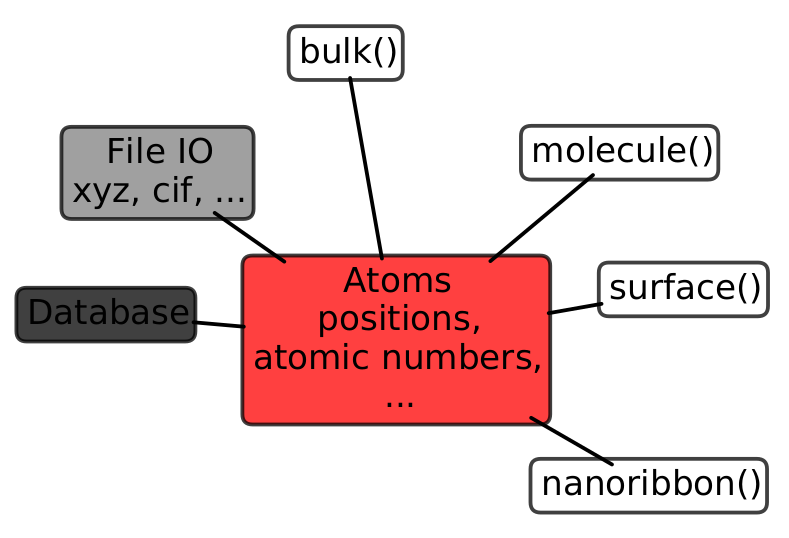
\includegraphics[height=1.3in,width=1.9in,viewport=0 0 820 530,clip]{Figures/ASE_atoms_module.png}
%\caption{\fontsize{7.2pt}{4.2pt}\selectfont{\textrm{The integrated calculator in ASE (Atomic Simulation Environment).}}}%
\label{Logo_atoms-module}
\end{figure} 
\hfill
\end{minipage}
\begin{minipage}[b]{0.50\textwidth}
\begin{figure}[h!]
\centering
\vspace*{-0.15in}
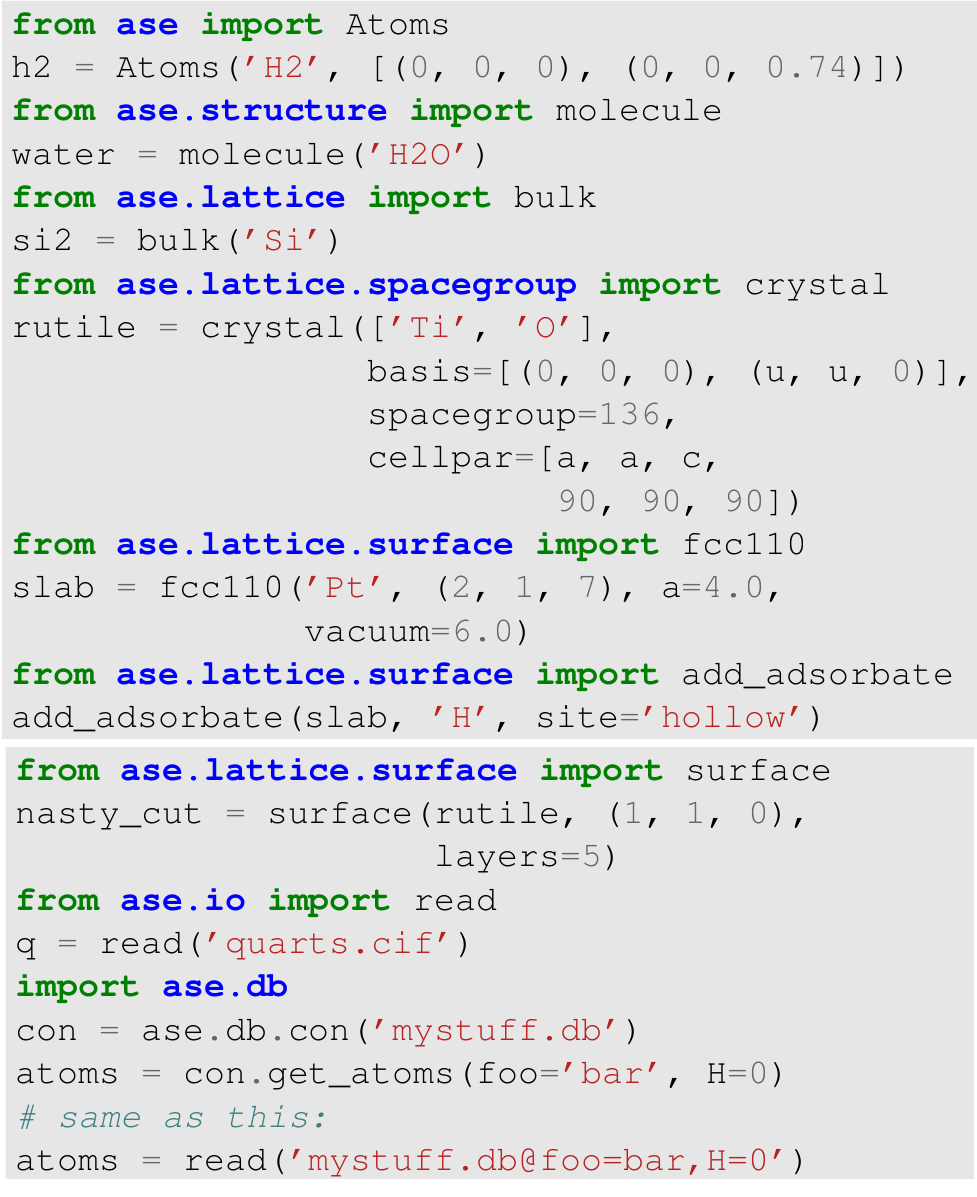
\includegraphics[height=2.9in,width=2.2in,viewport=0 0 970 1200,clip]{Figures/ASE_atoms_module-examples.png}
%\caption{\fontsize{7.2pt}{4.2pt}\selectfont{\textrm{The integrated calculator in ASE (Atomic Simulation Environment).}}}%
\label{Logo_atoms-module}
\end{figure} 
\end{minipage}
}

\frame
{
\frametitle{\textrm{ASE}特色:~软件接口丰富}
\textrm{Calculator}模块支持的可选软件
\begin{figure}[h!]
\centering
\vspace*{-0.05in}
%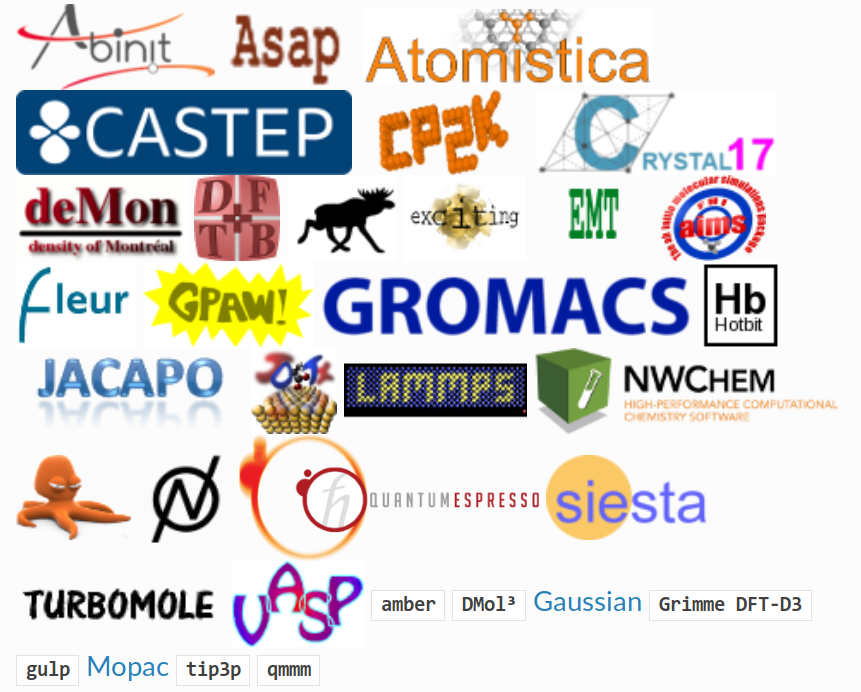
\includegraphics[height=1.0in,width=1.4in,viewport=0 0 638 530,clip]{Figures/ASE_calculator.png}
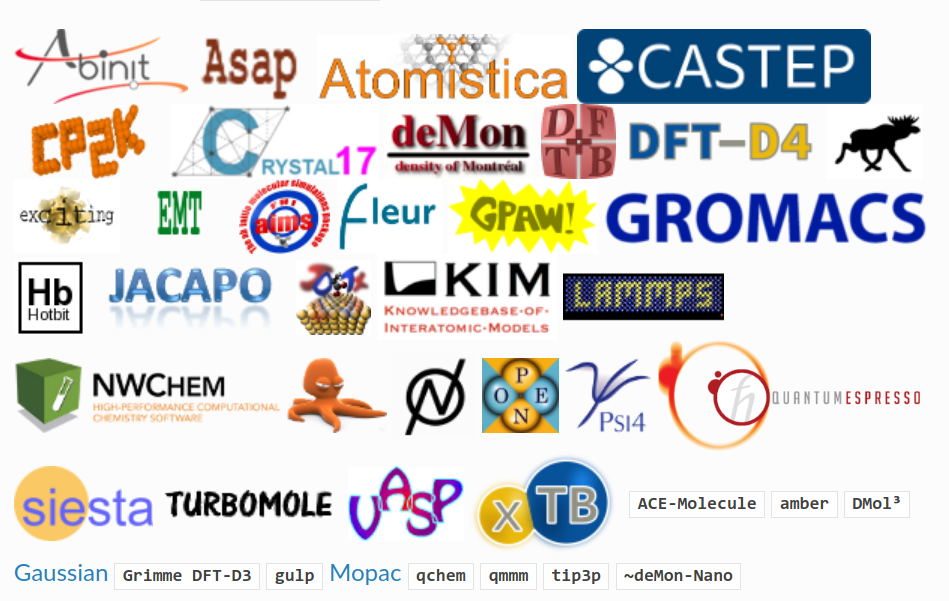
\includegraphics[height=2.4in,width=3.8in,viewport=0 0 940 600,clip]{Figures/ASE_calculator-new.png}
\caption{\fontsize{6.2pt}{4.2pt}\selectfont{\textrm{The integrated calculator in ASE.}}}%
\label{ASE_Calculator}
\end{figure} 
}

\frame
{
	\frametitle{\textrm{ASE}的模块:~\textrm{Calculator}和\textrm{checkpointing}}
\textrm{Calculator}:~支持各类计算软件的主要模块
	{\fontsize{8.0pt}{5.2pt}\selectfont{
\begin{itemize}
	\item 模块封装了\textrm{DFT-MD}计算软件,支持物性计算、功能分析
	\item 模块集成了全局结构搜索算法(\textrm{Base-hopping}和\textrm{minima-hopping}算法)、反应动力学模拟\textrm{NEB}算法和势能面鞍点搜索算法、\textrm{MD}模拟算法、几何结构优化算法和分子振动与声子振动分析算法
	\item 模块支持材料物性自动化计算,数据以标准化形式存入数据库
\end{itemize}
		模块启动计算依次执行以下步骤:
\begin{enumerate}
	\item 生成计算软件所需的输入(控制)文件
	\item 启动软件,以子进程方式开始计算过程
	\item 进程守护直至计算子进程结束
	\item 根据要求解析计算软件生成文件,并可将计算结果以\texttt{json}格式写入数据库
\end{enumerate}}}
{\fontsize{7.5pt}{5.2pt}\selectfont{
	\begin{itemize}
		\item \textcolor{red}{优点}:~\textrm{Python}模块与计算软件的交互简单
		\item \textcolor{red}{缺点}:~\textrm{Python}执行过程中会面向较多的\textrm{I/O}处理,运行效率不高
	\end{itemize} }}
\textrm{checkpointing}:~协助用户排查、定位错误和重启计算的模块
\vskip 2pt
{\fontsize{7.5pt}{5.2pt}\selectfont{增加\textrm{ASE}对计算流程的控制能力}}
}

\frame
{
\frametitle{\textrm{ASE}特色:~数据库的良好兼容性}
\begin{minipage}[b]{0.38\textwidth}
{\fontsize{7.5pt}{5.2pt}\selectfont{
\textrm{ASE}的材料数据库\textrm{CMR}采用关系型数据库管理系统\textrm{MySQL}
\vskip 1pt
{\fontsize{6.0pt}{5.2pt}\selectfont{将规范化的数据转成数据库文件(称为\textit{cmr}-文件),并要求数据库中的文件名尽可能与原文件保持一致}}
\begin{itemize}
	\item 用户不进入数据库即可对数据进行检验
	\item 存储数据有更大的兼容性
	\item 
	\item
\end{itemize}}}
\end{minipage}
\hfill
\begin{minipage}[b]{0.60\textwidth}
\begin{figure}[h!]
\centering
\vspace*{-0.10in}
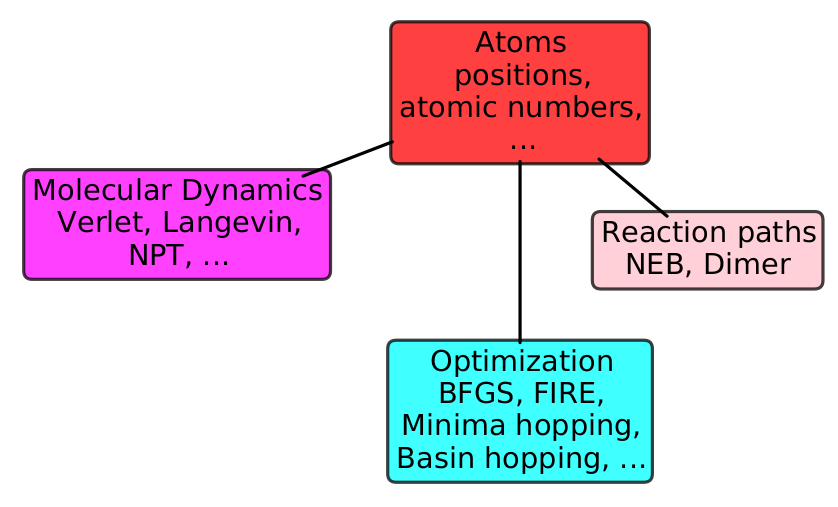
\includegraphics[height=1.3in,width=2.5in,viewport=0 0 838 500,clip]{Figures/ASE_opt_modules.png}
\vskip 1pt
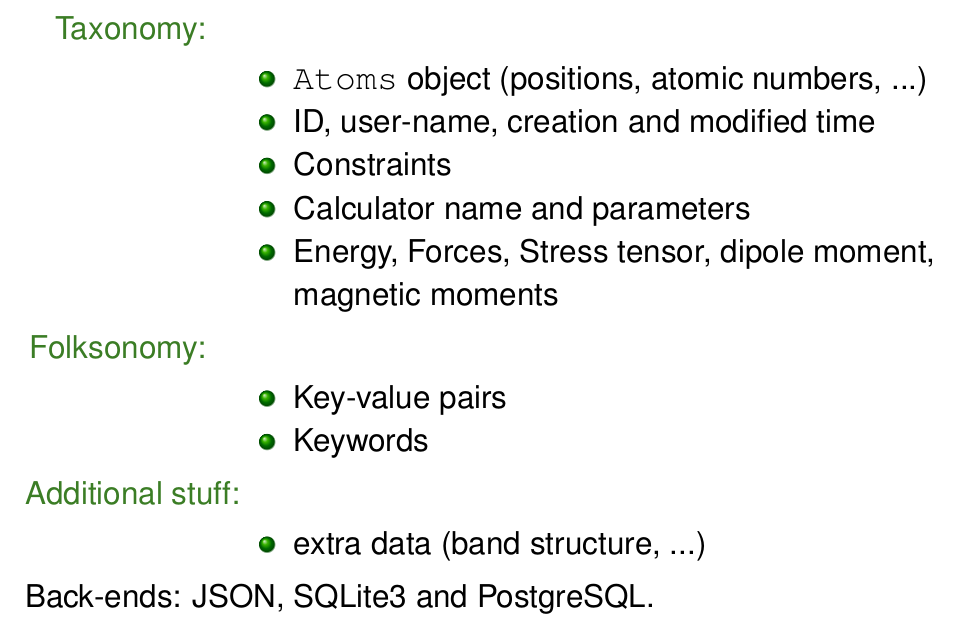
\includegraphics[height=1.7in,width=2.5in,viewport=0 0 938 630,clip]{Figures/ASE_database.png}
\label{ASE_opt-database}
\end{figure} 
\end{minipage}
}

\frame
{
	\frametitle{\textrm{MP}自动流程的架构}
流程标准化型的自动处理以\textrm{MP}的流程控制\textrm{FireWorks}为代表
	\begin{itemize}
		\item \textcolor{red}{设计目标}:~围绕\textrm{VASP~}作业高通量并发提交与过程监控
		\item \textcolor{red}{设计方案}:~开发针对不同计算场景的功能模块
			\begin{enumerate}
    \setlength{\itemsep}{7pt}
				\item \textcolor{blue}{\textbf{Pymatgen}}\\
					\textcolor{magenta}{前处理}:~计算模型的分析与预处理\\
					\textcolor{magenta}{后处理}:~计算结果的可视化
				\item \textcolor{blue}{\textbf{FireWorks}}\\
					\textcolor{magenta}{数据库支持的计算流程设计与管理}:~复杂的工作流可以数据形式保存到\textrm{MongoDB}数据库中,用\textrm{FireWorks}设计的工作流具有较高的稳定性
				\item \textcolor{blue}{\textbf{Custodian}}\\
\textcolor{magenta}{计算流程容错与应对}:~提供计算过程错误判断接口,由用户提供解决策略和针对性设计
			\end{enumerate}
	\end{itemize}
		%\item 计算过程的控制方式
}

\frame
{
	\frametitle{\textrm{Pymatgen}的模块结构}
\begin{figure}[h!]
\centering
\vspace*{-0.1in}
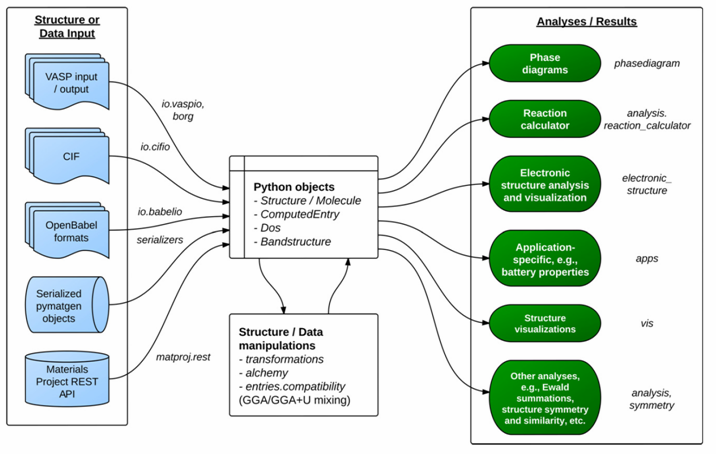
\includegraphics[height=2.3in]{Figures/MP_library.png}
\caption{\fontsize{7.2pt}{4.2pt}\selectfont{\textrm{Overview of a typical workflow for pymatgen.}}}%
\label{Pymatgen_Lib}
\end{figure} 
}

\frame
{
	\frametitle{\textrm{Pymatgen}可展示的材料物性}
\begin{figure}[h!]
\centering
\vspace*{-0.1in}
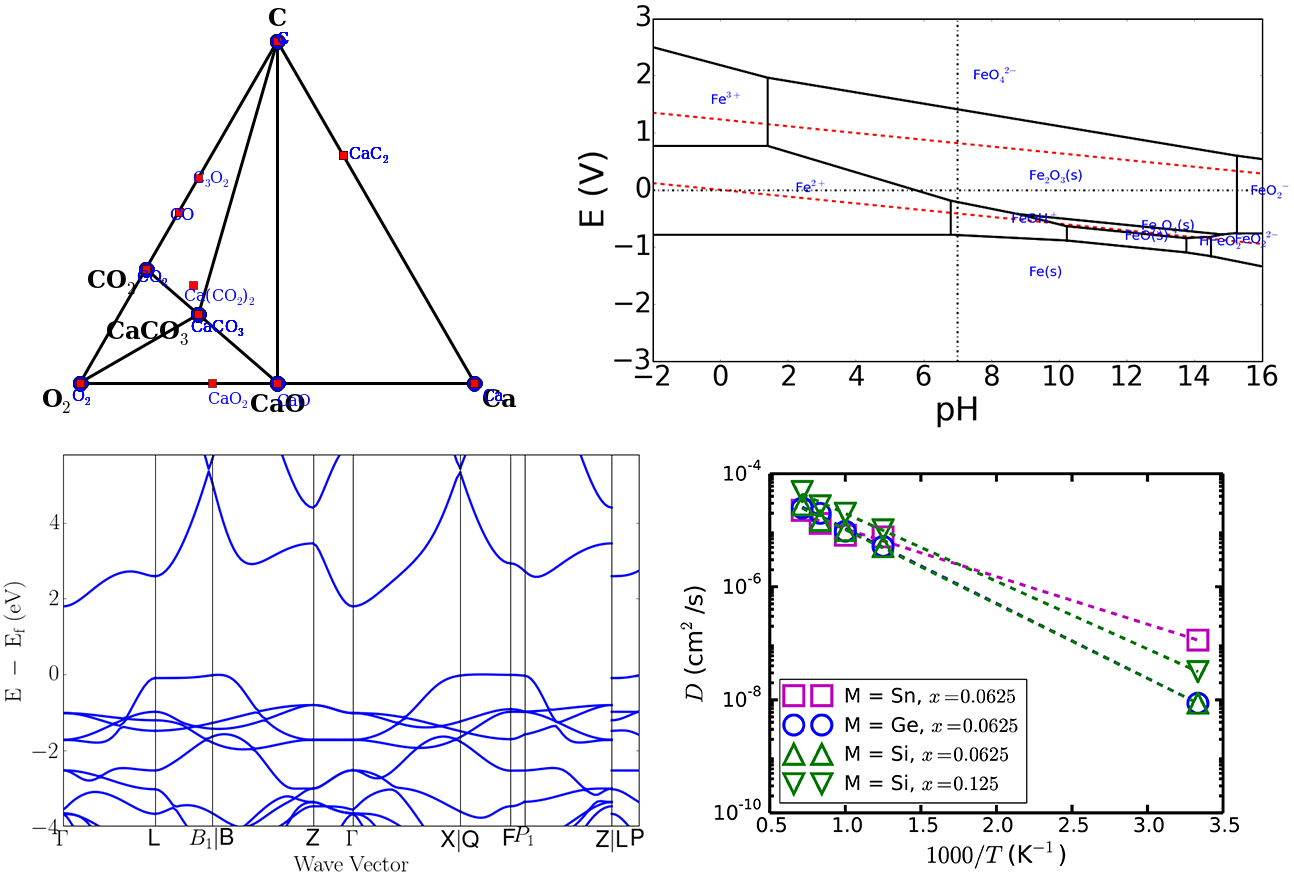
\includegraphics[height=2.3in]{Figures/MP_vision.png}
\caption{\fontsize{5.2pt}{4.2pt}\selectfont{\textrm{Top left: Phase; Top right: Pourbaix diagram from the Materials API. \\Bottom left: Calculated bandstructure plot using pymatgen’s parsing and plotting utilities. Bottom right: Arrhenius plot using pymatgen’s Diffusion~Analyzer.}}}%
\label{Pymatgen_vision}
\end{figure} 
}

\frame
{
	\frametitle{\textrm{FireWorks}的模块结构}
\textrm{FireWorks}是一款开源的通用工作流定义、管理和执行软件,支持\textrm{Python}运行
\vskip 3pt
\textrm{FireWorks}的自动流程采取中心化的“发布-执行”模式
\begin{itemize}
    \setlength{\itemsep}{7pt}
	\item 流程发布(称为\textrm{LaunchPad}):\\
		{\fontsize{7.2pt}{4.2pt}\selectfont{\textrm{LaunchPad}是工作流的主管者,主要负责自动流程的定义、分发、排队、增删和对工作流的反馈与响应}}
	\item 流程执行(称为\textrm{FireWorkers}):\\
		{\fontsize{7.2pt}{4.2pt}\selectfont{\textrm{FireWorkers}是工作流的执行者,包括一个或多个计算资源(个人计算机、小型工作站、超级计算机等)}}
\end{itemize}
\textrm{FireWorkers}从\textrm{LaunchPad}处获得计算任务,执行完毕后再将计算结果返回到\textrm{LaunchPad}
}

\frame
{
	\frametitle{\textrm{FireWorks}的模块结构}
\begin{figure}[h!]
\centering
\vspace*{-0.05in}
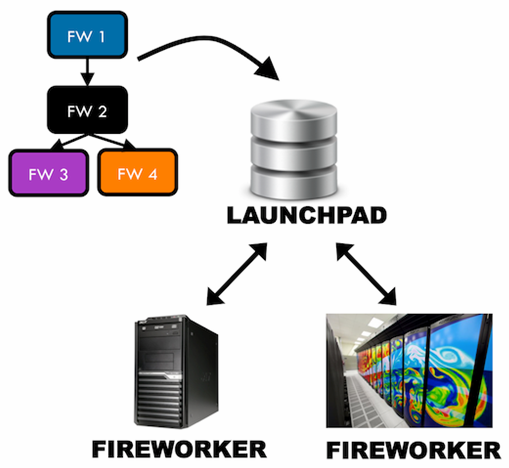
\includegraphics[height=1.5in]{Figures/MP_fireworks.png}
\hskip 1pt
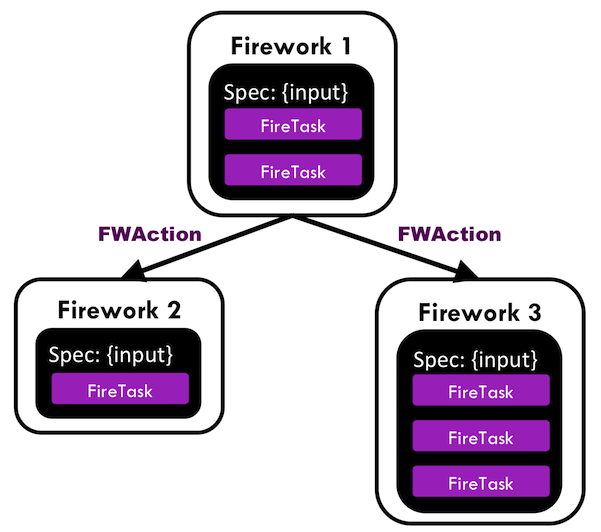
\includegraphics[height=1.5in]{Figures/MP_multiple_fw.png}
\caption{\fontsize{7.2pt}{4.2pt}\selectfont{\textrm{The basic infrastructure of FireWorks.}}}%
\label{FireWorks_FW}
\end{figure} 
\textrm{FireWorks}发布的工作流程由三层嵌套结构组成:
\fontsize{8.2pt}{6.2pt}\selectfont{
\begin{itemize}
	\item \textrm{Firetask}:~基本执行单元,是执行计算的最基本脚本命令或\textrm{Python}命令。
	\item \textrm{Firework}:~组织基本执行单元构成任务单元组,并指定各基本执行单元所需的参数。
	\item \textrm{Workflow}:~彼此相关联的任务单元组构成完整的工作流程:\\
		\textrm{FireWork}之间的数据传递、任务执行序列等由\textrm{FWAction}完成。
\end{itemize}}
}

\frame
{
	\frametitle{\textrm{FireWorks}的模块结构}
\fontsize{8.2pt}{6.2pt}\selectfont{
	\begin{itemize}
		\item \textrm{FireWorks}是以任务单元组为基本组成的来实现工作流程的,任务单元组之间依靠数据传递相关联,流程执行完毕也将返回数据,\textrm{FWAction}模块主要负责任务单元组之间的数据传递和任务分配。
		\item \textrm{FWAction}允许用户根据需要设计和更改流程参数、增添、删减和改变流程(子)单元组,这一模块大大增加了\textrm{FireWorks}工作流的灵活性。
	\end{itemize}}
\begin{figure}[h!]
\centering
\vspace*{-0.10in}
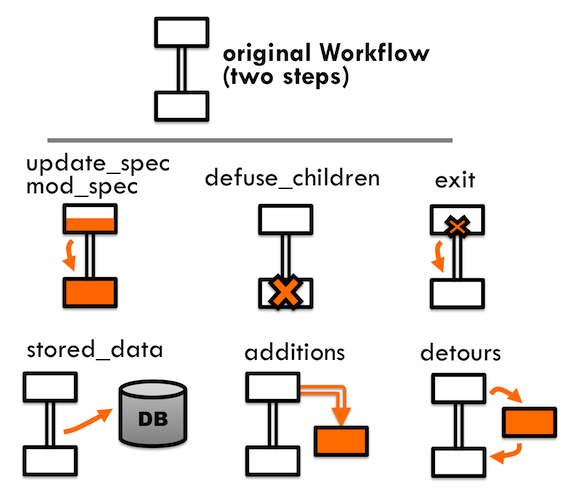
\includegraphics[height=1.9in]{Figures/MP_Fireworks_fwactions.png}
\caption{\fontsize{7.2pt}{4.2pt}\selectfont{\textrm{Schematic diagram for data transfer and processing between unit in FireWorks}.}}%
\label{FireWorks_FWA}
\end{figure} 
}

\frame
{
	\frametitle{\textrm{FireWorks}的模块结构}
这种“发布-执行”结构使得计算任务与软件、硬件高度解耦,用户可根据需要随时向\textrm{LaunchPad}添加新的工作流,承担计算任务的\textrm{FireWorkers}彼此也可以是完全异构的,具有很好的机动性。
\vskip 0.25in
对于材料第一原理计算自动流程而言,一个\textrm{DFT}计算过程就是一个\textrm{Firework},可以分解为:
\begin{enumerate}
	\item 指定控制参数:~参数在数据库\texttt{Json}中存储,由\textrm{Spec}传入
	\item 计算控制文件生成:~每个\textrm{Firetask}生成一个控制文件
	\item \textrm{DFT}计算作业提交:~产生一个\textrm{Firetask}
\end{enumerate}
在此基础上,可以通过\textrm{FWAction}修改控制参数,将\textrm{DFT}计算单元组组织成完整的材料第一原理计算流程,并将最终结果直接导入材料计算数据库。
}

\frame
{
	\frametitle{\textrm{Custodian}的容错逻辑}
\begin{figure}[h!]
\centering
\vspace*{-0.1in}
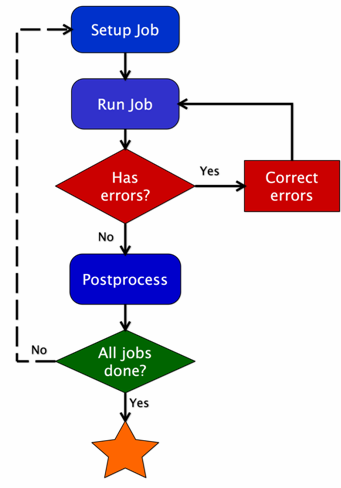
\includegraphics[height=2.7in]{Figures/MP_custodian.png}
\label{Custodian_over}
\caption{\fontsize{7.2pt}{4.2pt}\selectfont{\textrm{Overview of the Custodian workflow.}}}%
\end{figure} 
}

\frame
{
	\frametitle{\textrm{atomate}:~计算流程控制示范}
%		\textcolor{purple}{\textrm{Atomate}}:~:~适合一定复杂程度的\textrm{~VASP~}计算
\begin{figure}[h!]
\centering
\vspace*{-0.19in}
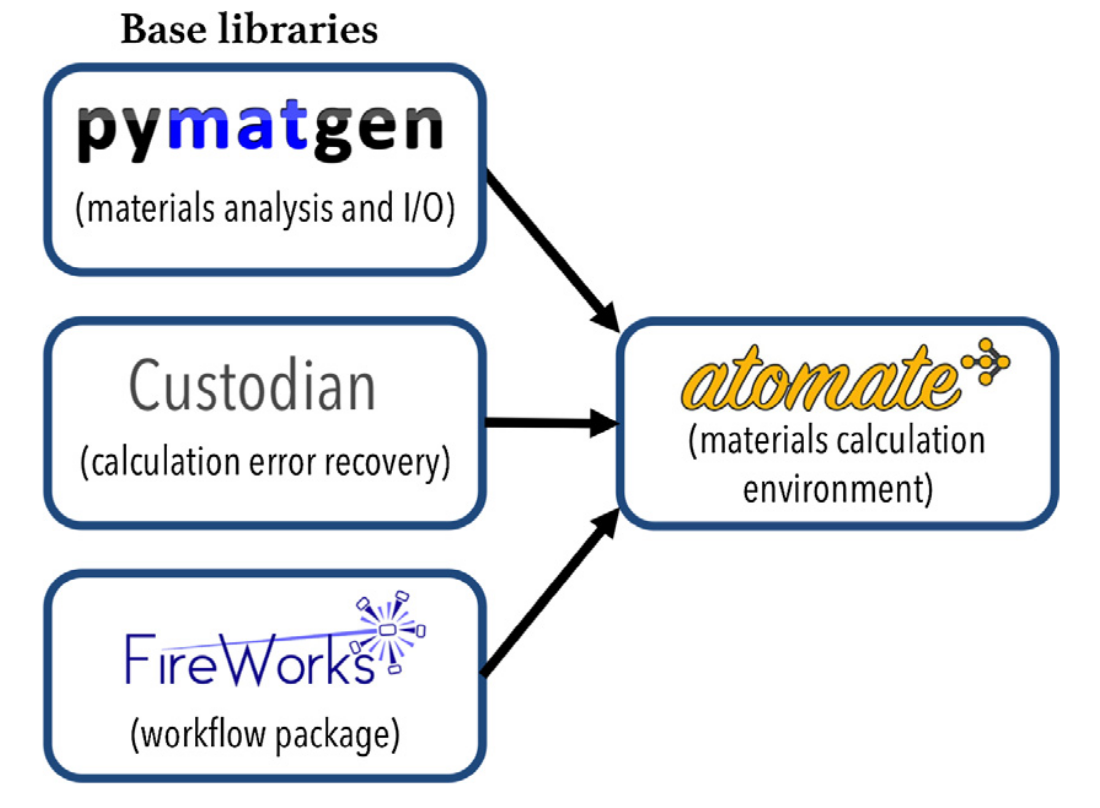
\includegraphics[height=1.4in,width=2.2in,viewport=0 0 820 630,clip]{Figures/Atomate_comp.png}
\vskip 1pt
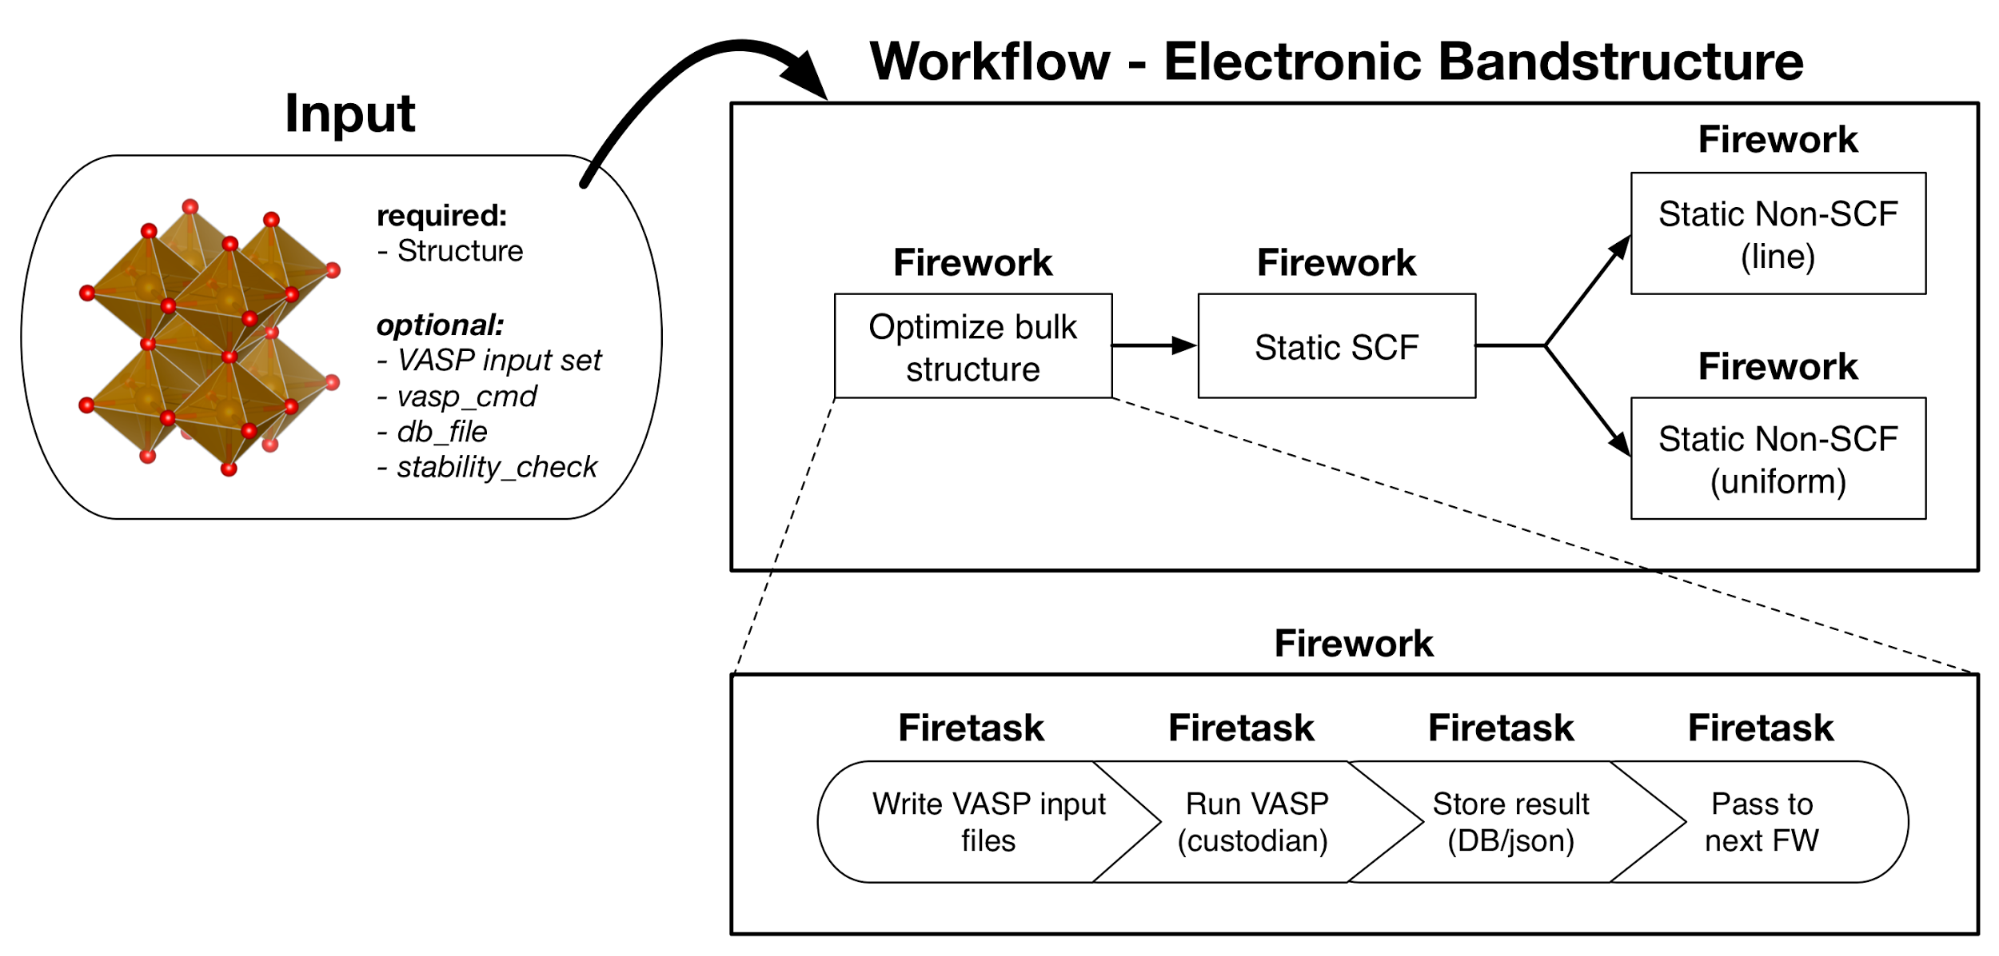
\includegraphics[height=1.5in]{Figures/bandstructure_wf.png}
%\caption{\fontsize{7.2pt}{4.2pt}\selectfont{\textrm{The integrated calculator in ASE (Atomic Simulation Environment).}}}%
\label{Logo_QM-MM}
\end{figure} 
}

\section{第一原理数据库}
\frame
{
	\frametitle{早期材料数据库:~\tt{SpingerMaterials}}
\textrm{SpingerMaterials}:~世界上最古老也是完备的材料数据库,旨在创建集成材料学信息、性质和使用平台
\vskip 3pt
数据库主要由以下部分组成:
\begin{itemize}
	\item 全部\textrm{Landolt-B{\"o}rnstein}丛书(自\textrm{1883}年起),是以基础科学为主的大型科学与技术数值与函数关系的工具书
	\item 全部\textrm{Pauling~File}无机材料数据库,收集了从\textrm{1900}年迄今超过\textrm{21000}种出版物中的无机晶体结构、衍射、相图和物理属性数据
	\item \textrm{Dortmud Data Band}中的纯液体和二元混合物的热物理数据
	\item 吸附材料数据库\textrm{(Adsorption Database)}
	\item 聚合物热力学数据库\textrm{(Polymer Thermodynamics Databse)}
	\item \textrm{MSI~Eureka}数据库:~无机材料相图、相反应和热力学数据
\end{itemize}
}

\frame
{
	\frametitle{早期材料数据库:~其它数据库}
除\textrm{SpingerMaterials}之外,比较完整的数据有
{\fontsize{9.0pt}{4.2pt}\selectfont{
\begin{itemize}
	\item 无机晶体结构数据库\textrm{(Inorganic Crystal Structure Database, ICSD)}:~\url{http://www.fiz-karlsruhe.com/icsd.html}%\cite{ICSD_URL},
		\vskip 2pt
{\fontsize{6.5pt}{4.2pt}\selectfont{服务器位于德国的\textrm{FIZ~Karlsruhe},收录了自\textrm{1913}年以来超过\textrm{185000}条矿物、 金属和其他无机固体化合物(含\textrm{2000}多元素单质、\textrm{34500}多二元化合物、\textrm{68000}多三元化合物、\textrm{66000}多四元及多元化合物)的晶体结构数据}}
%类似的实验材料数据库还有
\item \textrm{CRYSTMET}数据库%:~\url{http://www.tothcannda.com/database.htm}%\cite{CRYSTMET_URL}、
\item \textrm{Pauling}无机材料数据库:~\url{http://www.paulingfile.com/}%\cite{Pauling_URL}
\item \textrm{Pearson}晶体数据库:~\url{http://www.crystalimpact.com/}%\cite{Pearson_URL}
\item $\cdots$
\end{itemize}}}
\textcolor{blue}{这些实验数据库对于材料学研究提供了重要的帮助}

%但是仅有这些数据库肯定是不够的,一方面
\begin{itemize}
	\item 材料的覆盖范围非常广泛,有限的数据库不可能穷尽%,更重要的是
	\item 有很多材料的物性数据很难通过实验直接得到
\end{itemize}

%材料设计和开发是复杂的多维优化问题,注定新材料研发耗时耗力%。在这一点上,
原子尺度的材料物性数值模拟可以有效补偿实验方法的不足\\
%近年来雨后春笋般的计算材料数据库填补了不少很多实验数据缺乏的空白%\cite{CMS58-227_2012},
\textcolor{red}{集成了实验数据和计算数据的新材料数据库为探索新材料合成、性能优化开辟了新的研究思路}

%随着高性能计算与\textrm{DFT}相结合推动了第一原理材料模拟数据生成和结果分析的自动化,%而随着“材料基因组计划”的实施,为计算材料科学提供了越来越广阔的应用空间,也
%涌现了越来越多的计算材料数据库,特别是在功能材料领域,高通量\textrm{DFT}计算大大推进了新材料研发的进步。%\cite{JCED59-3232_2014, IC53-11849_2014,JPCL4-3607_2013,PCCP16-22073_2014}
}

\frame
{
\frametitle{\tt{AFLOWLIB}}
%\subsubsection{\tt{AFLOWLIB}}
\textrm{AFLOWLIB}是由高通量\textrm{DFT}计算框架\textrm{AFLOW}%\cite{CMS58-218_2012,CMS58-227_2012,Nat-Mater12-191_2013}
生成的材料信息数据库:~\url{https://www.aflowlib.org}
\vskip 3pt
{\fontsize{7.5pt}{4.2pt}\selectfont{该数据库涵盖相图、电子结构和磁学性质等信息,源代码和主要材料数据由\textrm{Duke}大学开发和运维}}%\cite{AFLOWORG_URL},
\begin{itemize}
	\item 数据库包含\textrm{630,000}种以上的合金热力学条目,涵盖了\textrm{ICSD}中的\textrm{52,000}多种化合物,\textrm{3,000}多种基本化合物,\textrm{330,000}多种二元化合物和\textrm{262,000}多种\textrm{Heuslers}金属间化合物
	\item 数据库提供在线的界面搜索,包括计算的细节、电子结构、磁学性质和热力学性质,所有的计算结果都是由\textrm{AFLOW}高通量计算软件生成的
	\item 计算数据在数据库种以\textrm{SQL}(\textrm{MySQL})形式存储,检索方便
		\vskip 2pt
		{\fontsize{7.5pt}{4.2pt}\selectfont{\url{https://www.aflowlib.org}~提供数据交换的应用接口\textrm{RESTful~API}服务}}%\cite{CMS93-178_2014},
\end{itemize}
数据库中的材料数据可以表示为多种格式,包括\texttt{HTML/JSON/DUMP/PHP/TEXT/NONE}等,极大地方便了用户在新材料研发中的数据挖掘需求
}

\frame
{
\frametitle{\tt{MP}}
%\subsubsection{\tt{MP}}
\textrm{Materials Project}是美国材料基因组项目项目支持高通量第一原理计算的软件和数据库:~\url{https://www.materialsproject.org}%\cite{MP_URL},
\vskip 2pt
{\fontsize{8.5pt}{4.2pt}\selectfont{\textrm{MP}基于\textrm{Apache}、\textrm{Python}和\textrm{Django}开发,在开源软件平台\textrm{github}上发布全部代码,面向全世界的开发者支持:~\url{https://gitbub.com/materialsproject}}}
\vskip 3pt
根据\textrm{MP}官网信息,目前可提供的数据包括:
\begin{itemize}
	\item \textrm{59,000}多种化合物的信息,\textrm{41,000}多种能带结构数据和\textrm{1,300}多种材料的弹性张量数据
	\item \textrm{2,200}多种\textrm{\ch{Li}}的插层电极和\textrm{19,000}多种\textrm{\ch{Li}}的转换电极数据
	\item \textrm{Materials Project}的扩展性极好\\
		{\fontsize{8.0pt}{4.2pt}\selectfont{除了\textrm{Pymatgen}、\textrm{FireWorks}和\textrm{Custodian}的支持,其数据库采用基于\textrm{MongoDB}的\textrm{NoSQL}数据格式文件,%因为传统的数据库只是“纵向可扩展”\footnote{\fontsize{5.0pt}{4.2pt}\selectfont{横向可扩展,是指数据库可支持增加数据库的服务器数目;~纵向可扩展是指数据库可支持增加硬盘、内存和\textrm{CPU}的数目}},\textrm{NoSQL}数据库
	弥补了传统数据库的扩展性差和灵活性不够的问题}}%,近年来在材料研究数据库技术中特别受到注意
\end{itemize}

\textrm{Materials Project}同样通过\textrm{API}支持\textrm{RESTful}服务%\cite{CMS68-314_2013},
%根据\textrm{RESTful}的设计,对数据的需求和操作,不须依赖复杂的用户界面,只要直接对数据库的\textrm{URL}完成。\textrm{RESTful}接受到\textrm{URL},\textrm{Materials Project}材料数据库返回的\textrm{JSON}结构。\textrm{RESTful}服务器有效地提升了数据获取效率,如\textrm{Pymatgen}的结构对象,\textrm{生成能}、\textrm{VASP}计算结果等。对科研工作者而言,\textrm{RESTful}是有效的研究工具。
}

\frame
{
\frametitle{\tt{CMR}}
%\subsubsection{\tt{CMR}}
\textrm{CMR}和\textrm{ASE}都是由丹麦技术大学\textrm{QMIP}项目开发的\\
{\fontsize{7.5pt}{4.2pt}\selectfont{\textrm{ASE}主要服务第一原理计算任务生成、计算执行、结果分析和可视化}}\\
\textrm{CMR}则主要面向计算数据存储:~\url{https://cmr.fysik.dtu.dk}
%{\fontsize{8.5pt}{4.2pt}\selectfont{当前\textrm{ASE}和\textrm{CMR}仍在开发中,不断发布更新的稳定版本}},有比较完整的安装、使用说明文档。
\begin{itemize}
	\item \textrm{CMR}提供了超过\textrm{30,000}条数据记录
	\item \textrm{CMR}提供了三种不同的用户界面\textrm{PHP/HTML和Python},方便不同经验的用户存储、检索电子结构计算数据%\cite{CMR_URL},\cite{CSE14-51_2012},
\end{itemize}
与\textrm{ASE}类似,\textrm{CMR}面向用户对数据库的多元化需求,实现软硬件的尽可能兼容
{\fontsize{7.5pt}{4.2pt}\selectfont{
\begin{itemize}
	\item 软件方面:~\textrm{ASE}和\textrm{CMR}所有源代码开发都是基于松耦合模式,方便用户根据习惯使用软件\\
		{\fontsize{6.0pt}{4.2pt}\selectfont{主要是面向开源系统,特别是\textrm{Linux}操作系统,\textrm{Apache}浏览器,\textrm{MySQL}数据库,用户界面采用\texttt{PHP/HTML},合成\textrm{LAMP}(\textrm{Linux,Apache,MySQL,PHP})套装}}
		%。比如用户可以分别只选用\textrm{ASE}或\textrm{CMR};
	\item 硬件方面,软件可以安装到台式机、集群或超级计算机上,对于小的台式机则无须安装数据库和网络服务器
	\item \textrm{CMR}使用\textrm{SQLite}数据库模式而不用\textrm{MySQL}服务器模式存储和检索材料数据\\
		{\fontsize{6.0pt}{4.2pt}\selectfont{当用户有需要时,\textrm{CMR}的数据处理模块可将\textrm{SQLite}数据库文件上传到\textrm{MySQL}服务器上,或者将数据文件转呈\texttt{XML/JSON}格式,以方便数据交换}}
\end{itemize}}}
}

\frame
{
\frametitle{\tt{ESP}}
%\subsubsection{\tt{ESP}}
\textrm{ESP}的数据库是\textrm{Uppsala}大学为加速新的功能材料的研发进程而开发的:~\url{http://gurka.fysik.uu.se/ESP/}
\begin{itemize}
	\item \textrm{ESP}数据库中的电子结构数据是依据\textrm{ICSD}的无机化合物的结构数据,由\textrm{FP-LMTO}方法通过第一原理计算产生\\
{\fontsize{6.5pt}{4.2pt}\selectfont{自2002年\textrm{ESP}发布以来,共收录了\textrm{60,000}多条化合物的电子结构数据}}
\item 用户最多允许查阅含有五种元素的化合物的电子结构信息
\end{itemize}
应用数据挖掘技术,由\textrm{ESP}的\textrm{60,000}多条化合物电子结构信息,已经预测了17种潜在可能的强拓扑绝缘体\\%\cite{arXiv1007-4838_2010,APR6-31_2014},
{\fontsize{7.5pt}{4.2pt}\selectfont{\textrm{ESP}的官网提供的信息显示:~采用大规模计算结合数据挖掘技术提供的17种可能的化合物中,成功预测到了第一个强拓扑绝缘体\textrm{(toplogical insulator)}\textrm{\ch{Bi2SeTe2}},而且预测很快就得到验证}}

\textrm{ESP}的数据库和能带分析工具的代码都没有公开\\
近年来,\textrm{ESP}数据库开发进展缓慢
}

\frame
{
\frametitle{\tt{ESTEST}}
%\subsubsection{\tt{ESTEST}}
\textrm{ESTEST}是加州大学\textrm{Davis}分校%\textrm{(the University of California at Davis)}
开发的材料数据库:\\\url{http://estest.ucdavis.edu/}\\%\cite{ESTEST_URL,CSD3-015004_2010,CPC183-1744_2010}
{\fontsize{6.5pt}{4.2pt}\selectfont{用于软件\textrm{Qbox}、\textrm{VASP}、\textrm{Quantum Espresso}、\textrm{Siesta}、\textrm{ABINI}的结果和电子结构计算软件\textrm{Exciting}的结果检验和对比}}

通过数据库的网页界面,可将各类软件的输入/输出文件转换成统一的\textrm{XML}格式,便于数据存储、比较、分析\\
{\fontsize{6.5pt}{4.2pt}\selectfont{每个\textrm{XML}文件由文件名和数据库存储位置区别}}
{\fontsize{7.5pt}{4.2pt}\selectfont{
\begin{itemize}
	\item \textrm{ESTEST}数据库总共包括\textrm{400}多条\textrm{Qbox}的计算记录,\textrm{10}条左右的\textrm{VASP}计算记录,\textrm{Quantum Espresso}和\textrm{Siesta}计算记录各\textrm{70}多条,\textrm{150}多条\textrm{ABINIT}计算记录,\textrm{Exciting}的记录约\textrm{30}条
	\item \textrm{ESTEST}的网页界面提供了类似\textrm{Google}的简明搜索栏,网页还提供了多个搜索下来菜单,可根据软件名称、计算元素等检索

	\item 数据库的网页界面可提供数据、表格和图片形式的电子结构的模拟信息:\\
		{\fontsize{6.5pt}{4.2pt}\selectfont{包括计算参数、原子信息、能量结果和结构应力与光谱信息}}

	\item 网页界面还提供了一些插件,可对诸如原子距离、晶格、能带结构、态密度、能量和结构应力或其他记录转换成一种或多种数据格式\\
{\fontsize{6.5pt}{4.2pt}\selectfont{例如\textrm{band\_structure\_plot}插件可将\textrm{XML}格式的能量本征值转成电子能带图}}\\
\end{itemize}
这种格式转换插件丰富了\textrm{ESTEST}生成、模拟计算结果的能力\\
需要说明的是:~必须是注册用户才能数据库的源代码}}
}

\frame
{
\frametitle{\tt{MAST}}
%\subsubsection{\tt{MAST}}
以完整的高通量框架的角度看,\textrm{MAST}更像是对\textrm{ESTEST}的辅助,重点用于工作流管理和后处理:\\
\url{http://pythonhosted.org/MAST/0_0_introduction.html}

\textrm{MAST}的基本框架由\textrm{MP}的\textrm{Pymatgen}和\textrm{Custodian}模块和\textrm{ASE}组合搭配实现
\vskip 2pt
{\fontsize{6.5pt}{4.2pt}\selectfont{\textrm{MAST}开发了自动计算流程以及数据库,而没有使用\textrm{FireWorks}和\textrm{MangoDB}}}
\vskip 2pt
\textrm{MAST}的数据主要来自\textrm{VASP}的数据拟合\\

\begin{itemize}
	\item \textrm{MAST}的数据库主要收集了带空位的稳定纯元素的数据,现有面心立方的\textrm{49}种元素和六方密堆积的\textrm{44}种元素
	\item \textrm{MAST}数据库主要用于研究基本的空位扩散,收集的数据包括:~空位形成焓、空位迁移焓、内聚能和体模量
\end{itemize}
\textrm{MAST}的数据生成和管理主要依赖于操作系统和\textrm{I/O}性能,运行\textrm{MAST}无须额外配置专门的数据库软件

\textrm{MAST}的数据目前还不能通过网页界面访问,很多功能还有待完善

}

\frame
{
\frametitle{\tt{CEPDB}}
%\subsubsection{\tt{CEPDB}}
\textrm{CEPDB}是哈佛大学的\textrm{CEP}项目的数据库:\\%\cite{CEPDB_URL,JPCL2-2241_2011}。
\url{https://gist.github.com/jessiegt/5642460f061a39d1820e}\\
主要服务于研究有机光电材料

根据\textrm{CEPDB}的网页信息显示,
\begin{itemize}
	\item 数据库共拥有\textrm{2,300,000}多个分子的图谱信息和\textrm{22,000,000}多个分子结构(由超过\textrm{150,000,000}个\textrm{DFT}计算得到)共计超过\textrm{400~TB}的数据,
	\item 数据库除了有第一原理计算结果,还收录了文献中的实验数据,用于作为\textrm{CEPDB}的训练和标定数据集
\end{itemize}
\textrm{CEPDB}使用\textrm{Python}的网页框架\textrm{Django}在\textit{in silico}上开发的高通量计算\textrm{MySQL}数据库,数据由量子化学计算软件\textrm{Q-Chem}得到\\
{\fontsize{6.5pt}{4.2pt}\selectfont{\textrm{CEPDB}的强大算力主要由\textrm{IBM}的公益分布式计算项目全球社群网格\textrm{(World Community Grid, WCG)}提供,还有一些算力来自\textrm{Harvard}的\textrm{FAS Odyssey}集群、\textrm{NERSC}和\textrm{TeraGrid}的计算资源以及其它一些计算资源}}

\textrm{CEPDB}的数据都是开放的,但高通量计算软件部分不开源\\不过\textrm{CEPDB}对全世界各研究组上传的实验数据持开放态度
}

\frame
{
\frametitle{\texttt{CCCBDB}}
%\subsubsection{\texttt{CCCBDB}}
计算化学对比和基准数据库\textrm{(Computational Chemistry Comparison and Benchmark Database, CCCBDB)}归属于美国国家标准和技术协会(\textrm{National Institute of Standards and Technology, NIST})

汇集了\textrm{1600}多种气相原子和分子的实验和第一原理计算的化学热力学数据,很好地弥补了常见数据库只有固体材料数据的不足

\begin{itemize}
	\item \textrm{CCCBDB}提供简单的在线服务界面,用户可以检索到指定化合物的实验数据和计算数据,实验和计算数据的对比也验证了数据的可靠性
	\item \textrm{CCCBDB}允许用户优先使用几何结构、振动模式、熵、能量和静电性质而非分子结构作为检索的关键词\\
		{\fontsize{7.5pt}{4.2pt}\selectfont{避免引入复杂的筛选组合,方便用户快速得到检索结果}}
	\item \textrm{CCCBDB}是一个庞大的数据库,收录了总计有超过\textrm{460,000}个计算条目\\
{\fontsize{7.5pt}{4.2pt}\selectfont{因为其没有开源,降低了数据库的影响力}}
\end{itemize}
}

\frame
{
\frametitle{\tt{AiiDA}}
%\subsubsection{\tt{AiiDA}}
\textrm{AiiDA}%\cite{AiiDA_URL}
是用于原子尺度材料自动模拟、管理、共享和复制的软件框架:~\url{http://www.aiida.net/}
\vskip3pt
{\fontsize{8.0pt}{4.2pt}\selectfont{软件由\textrm{THEOS-EPFL~(Theory and Simulation of Materials-{\'E}cole~Polytechnique~F{\'e}d{\'e}rale~de~Lausanne)}的实验室和\textrm{BOSCH}公司于2012年开发和维护}}
\vskip 3pt
\textrm{AiiDA}数据库
\begin{itemize}
	\item 网页编程框架用\textrm{Python}维护
	\item 数据库用\textrm{Django}开发\\%\cite{CMS187-110086_2021},
		{\fontsize{7.0pt}{4.2pt}\selectfont{可满足计算物理、化学和材料科学研究的多种不同需求}}
\end{itemize}
数据库提供\texttt{SQLite/MySQL}和\texttt{PostgreSQL}三种形式的数据
\vskip 3pt
{\fontsize{8.0pt}{4.2pt}\selectfont{推荐使用\textrm{PostgreSQL}}}
\vskip 5pt
当用户使用数据库的\textrm{RESTful~API}接口时,数据将以\texttt{JSON}格式呈现
}

\frame
{
\frametitle{\tt{Alloy Database}}
%\subsubsection{\tt{Alloy Database}}
\textrm{Alloy~Database}数据库
提供\textrm{VASP}计算的合金结构和结合能数据,%\cite{AlloyD_URL},
其在线服务器位于卡内基梅隆大学\textrm{(Carnegie~Mellon~University)}物理系:
\url{http://alloy.phys.cmu.edu}
\vskip 3pt
\textrm{Alloy~Database}数据库的主要功能
\begin{itemize}
    \setlength{\itemsep}{5pt}
	\item 包括\textrm{200}多种二元合金、\textrm{100}多种三元合金和\textrm{20}多种四元合金的材料数据
	\item 用户可以检索二元、三元和四元合金的\textrm{VASP}计算数据
	\item 数据库提供包括合金组分的元素信息、\textrm{Pearson}符号、合金模型以及计算所需的\textrm{POSCAR}文件、合金\textrm{Pearson}符号,基态总能和生成焓、化学组成和赝势等
\end{itemize}
\textrm{Alloy~Data}最早于\textrm{2006}年提供线上服务,由于其数据库服务代码从未开放,所以该数据库迄今尚未应用于高通量第一原理计算
}

\frame
{
\frametitle{\tt{NoMaD}}
%\subsubsection{\tt{NoMaD}}
{\fontsize{8.0pt}{4.2pt}\selectfont{
\textrm{Novel Materials Discovery~(NoMaD)}是面向第一原理计算的电子结构数据生成、组织和交换的重要材料数据库:~\url{http://nomad-repository.edu/cms/}%\cite{NoMaD_URL}。
\vskip 3pt
当前\textrm{NoMaD}数据库
\begin{itemize}
	\item 包含\textrm{640,000}多条数据\\
		{\fontsize{6.0pt}{4.2pt}\selectfont{其中有\textrm{250,000}多条数据来自~\url{http://aflowlib.org},其余则来自~\url{http://cccbdb.nist.gov}}}
	\item 通过网页~\url{http://nomad-repository.edu/gui/\#nomad}~共享数据
	\item 用户可通过元素、结构和计算方法、作者等信息检索到目标数据
	\item 供下载的数据主要是计算所需的输入/输出文件的压缩包\\
{\fontsize{6.0pt}{4.2pt}\selectfont{少量关于计算本身(如材料的化学式、空间群、计算软件及版本、作者和参考文献等)}}
\end{itemize}
{\fontsize{7.0pt}{4.2pt}\selectfont{\textrm{NoMaD}目前可支持的计算软件数据涵盖:~\textrm{ABINIT}、\textrm{CASTEP}、\textrm{CRYSTAL}、\textrm{Exciting}、\textrm{FHI-aims}、\textrm{Gaussian}、\textrm{Quantum-Espresso}、\textrm{VASP}和\textrm{WIEN2k}等}}
\vskip 3pt
{\fontsize{7.5pt}{4.2pt}\selectfont{\textrm{NoMaD}的注册用户不仅可以浏览和下载材料数据,还允许向\textrm{NoMaD}上传数据
\vskip 2pt
	{\fontsize{6.0pt}{4.2pt}\selectfont{用户可指定上传文件为“开放”\textrm{(open access)}或“限制”\textrm{(restricted)}状态}}
%\begin{itemize}
%	\item “开放”态:~对全体互联网用户开放
%	\item “限制”态:~只对指定用户群开放。
%\end{itemize}
\vskip 3pt
\textrm{NoMaD}的绝大部分数据(约\textrm{540,000}多条)是开放的,而“限制”状态的数据最多三年后自动转成“开放”状态,确保科学材料数据最大限度的共享和交换能力
\vskip 3pt
\textrm{NoMaD}除了提供材料计算的输入/输出文件,未提供高通量计算框架,一些重要的和有价值的材料数据{\fontsize{6.0pt}{4.2pt}\selectfont{(如计算参数以及计算能量数据)}}在数据文件下载之前已被隐去}}
}}
}

\frame
{
\frametitle{{\tt OQMD}与\tt{qmpy}}
%\subsubsection{\tt{OQMD}与\tt{qmpy}}
{\fontsize{8.0pt}{4.2pt}\selectfont{
开放量子材料数据库\textrm{(Open Quantum Materials Database, OQMD)}是\textrm{2013}年前后,由美国西北大学\textrm{(Northwestern University)}的研究团队在超过\textrm{200,000}个\textrm{DFT}计算的晶体结构基础上发展起来的:~\url{http://oqmd.org/}
\vskip 2pt
{\fontsize{6.0pt}{4.2pt}\selectfont{数据主要是在西北大学高性能计算队列和美国国家能源研究科学计算中心\textrm{(the National Energy Research Scientific Computing Center, NERSC)}的机器上完成}}

\begin{itemize}
	\item \textrm{OQMD}累积的\textrm{DFT}计算化合物约有\textrm{290,000}条
\vskip 2pt
{\fontsize{6.0pt}{4.2pt}\selectfont{这些化合物中约\textrm{10\%}来自\textrm{ICSD},约\textrm{90\%}来自简单化合物的组合,数据库中的化合物条目仍在增加}}
	\item 数据库收录的\textrm{DFT}计算的材料热力学和结构性质数据可以在线共享%\cite{OQMD_URL,NCM1-15010_2015},
	\item 数据库没有提供\textrm{RESTful}服务,但允许用户在\textrm{URL}地址栏输入检索化合物的字符串
		\vskip 2pt
		{\fontsize{6.0pt}{4.2pt}\selectfont{如~\textrm{\url{http://oqmd.org/materials/composition/Al2O3}}~表示\textrm{\ch{Al2O3}}的检索}}
\end{itemize}
{\fontsize{7.0pt}{4.2pt}\selectfont{软件\textrm{qmpy}是\textrm{OQMD}的\textrm{Python}的\textrm{API}:~\url{http://oqmd.org/static/docs/index.html}%\cite{qmpy_URL}
%和全部近\textrm{300,000}个结构数据可下载
\vskip 3pt
\textrm{qmpy}用\textrm{Django}开发,数据库是\textrm{MySQL}形式,数据主要由\textrm{VASP}计算得到}}
\vskip 5pt
通过浏览器得到的\textrm{OQMD}检索数据是\texttt{HTML}格式的(而非\texttt{JSON}或\texttt{XML}格式的)
\vskip 3pt
\textrm{OQMD}允许用户将全部数据(约4\textrm{GB})下载到本地并保存成一个文件,对于小型的计算用户,这将提升用户对计算数据的掌控和分析能力}}
}

\frame
{
\frametitle{\tt{PyChemia}}
%\subsubsection{\tt{PyChemia}}
{\fontsize{8.0pt}{4.2pt}\selectfont{\textrm{Python Materials Discovery Framework~(PyChemia)}是近年来才出现的面向\textrm{DFT}的高通量计算框架
\begin{figure}[h!]
\centering
\vspace*{-0.15in}
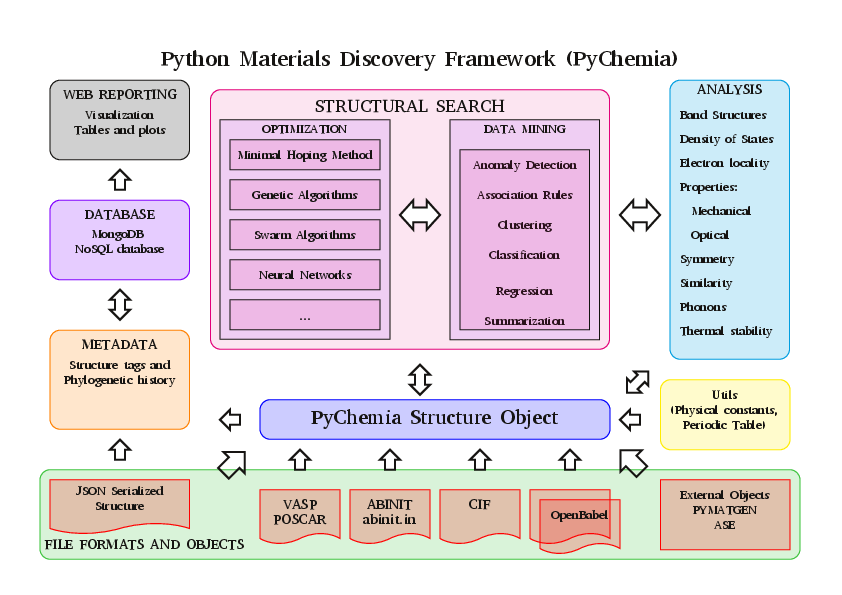
\includegraphics[height=2.3in]{PyChemia_code.png}
%\caption{\fontsize{7.2pt}{4.2pt}\selectfont{\textrm{The Framework of PyChemia.}}}%
\label{PyChemia_FireWork}
\end{figure} 
\textcolor{red}{目标}:~通过涵盖\textrm{DFT}计算和\textrm{Minima Hoping}等各种方法来推动发现新材料,并将\textrm{PyChemia}计算的数据存入数据库,作为后续发现新材料的备选化合物}}
}

\frame
{
\frametitle{\tt{PyChemia}}
{\fontsize{8.0pt}{4.2pt}\selectfont{\textrm{PyChemia}作为\textrm{Python}的一个模块,全部代码是最初于\textrm{2014}年由西弗吉尼亚大学\textrm{(West Virginia University)}分享到\textrm{GitHub}网站:\\
\url{http://github.com/MaterialsDiscovery/PyChemia}%\cite{PyChemia_Github},

\textrm{PyChemia}的新特色
\begin{itemize}
	\item \textrm{PyChemia}可支持的\textrm{DFT}计算软件涵盖\textrm{VASP}、\textrm{ABINIT}、\textrm{Octopus}、\textrm{DFTB+}和\textrm{Fireball}等
	\item 利用\textrm{Python}模块的特点,\textrm{PyChemia}完成了对\textrm{Pymatgen}、\textrm{ASE}和\textrm{qmpy}的集成
	\item 相比于其他高通量材料计算软件,\textrm{PyChemia}更显著的特长是材料结构搜索,而不是简单的材料计算和数据采集
		\vskip 2pt
		{\fontsize{6.0pt}{4.2pt}\selectfont{\textrm{PyChemia}除了提供大的材料数据库作为结构搜索的基础,还可以将每一套结构搜索产生新的小型数据库}}
\end{itemize}
\vskip 3pt
%图\ref{PyChemia_FireWork}给出了\textrm{PyChemia}的代码框架。
\textrm{PyChemia}采用\textrm{MongoDB}的\textrm{NoSQL}数据库而非传统的关系型数据库形式,方便产生结构搜索需要的小型数据库
\vskip 2pt
{\fontsize{6.0pt}{4.2pt}\selectfont{为兼顾不同\textrm{DFT}计算软件包材料结构以及各种物理性质研究的需要}}
\vskip 3pt
\textrm{PyChemia}由\textrm{Python}、\textrm{Django}和\textrm{MongoDB}搭建而成,其中\textrm{Django}是\textrm{PyChemia}用于显示计算的网页前端

目前\textrm{PyChemia}仍在开发中,尚未发布稳定版本的软件}}
}

\frame
{
	\frametitle{\tt{Atomly}}
\textrm{Atomly}材料科学数据库%\cite{ATOMLY_URL}
是中国科学院物理研究所刘淼、孟胜团队合作开发的第一原理材料数据库:~\url{https://www.atomly.net/}
\begin{figure}[h!]
\centering
\vspace*{-0.1in}
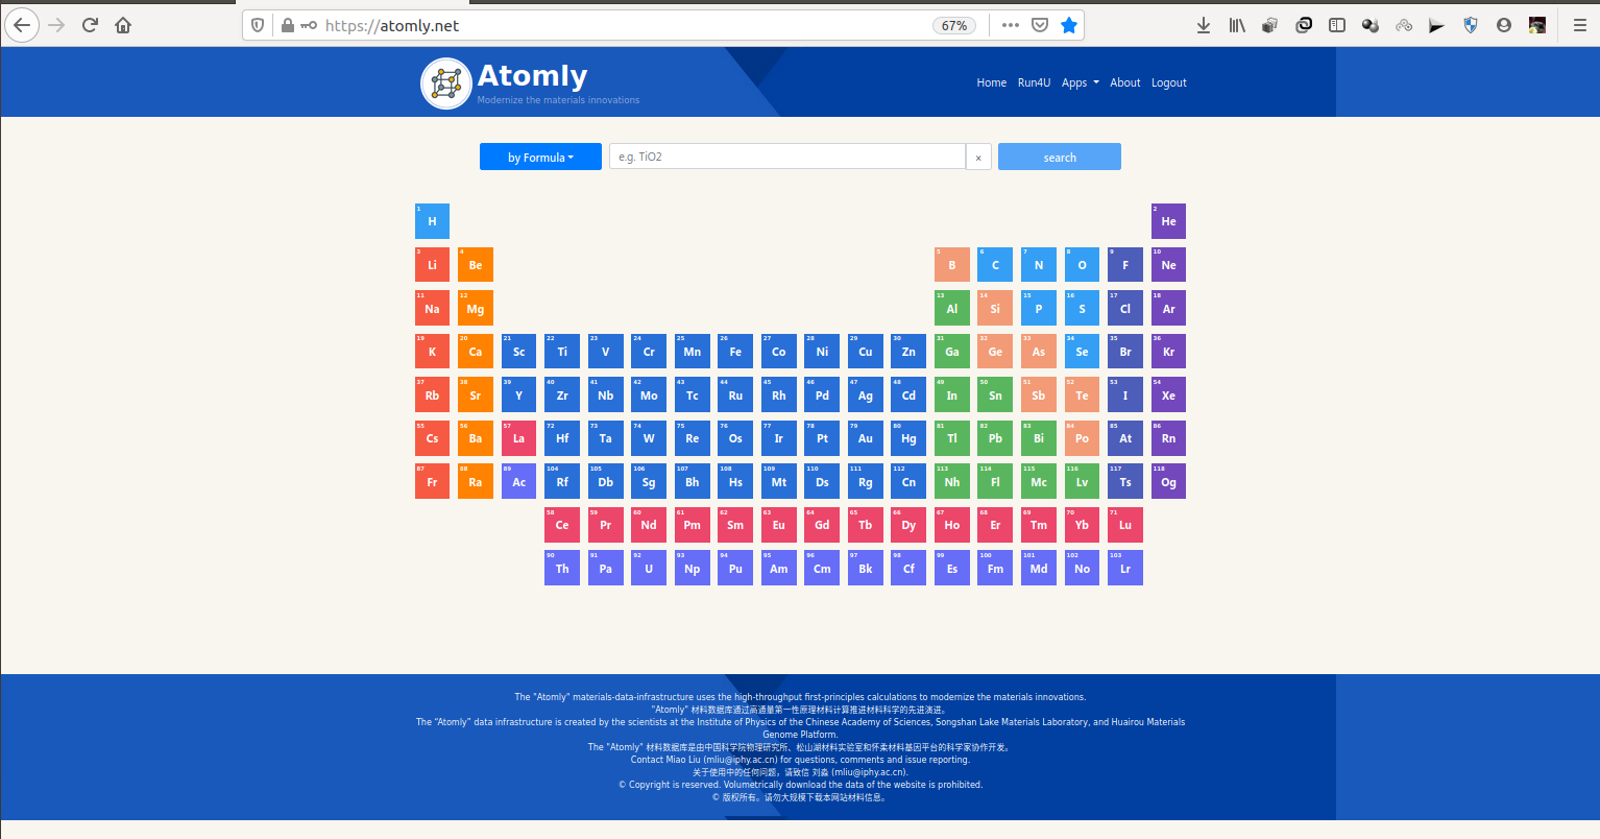
\includegraphics[height=2.1in,width=4.1in,viewport=5 0 1608 830,clip]{Figures/Atomly.png}
%\caption{\fontsize{7.2pt}{4.2pt}\selectfont{\textrm{Atomly:~中科院物理所~刘淼等老师开发,数据库包含了17万\!$^+$\!无机晶体材料第一性原理计算结果\textrm{(包含电子结构信息:~DOS~+~energy~bands)}.}}}%
\label{Logo_Atomly_lib}
\end{figure} 
}

\frame
{
\frametitle{\tt{Atomly}}
%\subsubsection{\tt{Atomly}}
%截止到目前已经收录了超过180,000条无机材料的高质量数据。
\textrm{Atomly}的\textcolor{red}{目标}:~为科研领域带来材料数据工具平台,通过数据驱动新材料的筛选、预测和发现,提升材料研发的生产力
\vskip 5pt
\textcolor{purple}{\textrm{Atomly}已收录\textrm{349,000+}种化合物,\textrm{342,00+}种能带结构和\textrm{68,000+}种相图数据}
\vskip 3pt
\begin{itemize}
	\item \textrm{Atomly}提供了性能优异的高通量第一原理计算流程框架\\
		{\fontsize{6.5pt}{4.2pt}\selectfont{依托中科院物理所的松山湖材料实验室的计算资源,框架支持的高通量计算流程可以支持~$10^3$数量级的材料体系同时计算}}
	\item \textrm{Atomly}的网页前端,提供便捷搜索,能快速定位到指定材料数据,并以友好的方式呈现给用户
	\item \textrm{Atomly}初步实践数据驱动的材料设计理念,能快速地完成高通量筛选,发现性能最优的候选材料
\end{itemize}
\vskip 5pt
借助人工智能算法,\textrm{Atomly}支持材料性质预测,能够以更快捷、更精准的范式预测材料结构和性质
}

\section{机器学习简介}
\frame
{
	\frametitle{机器学习\textrm{(Machine Learning, ML)}}
机器学习是自动完成数据分析并提取数据关系的一类方法的统称
\begin{figure}[h!]
\centering
\vspace*{-0.1in}
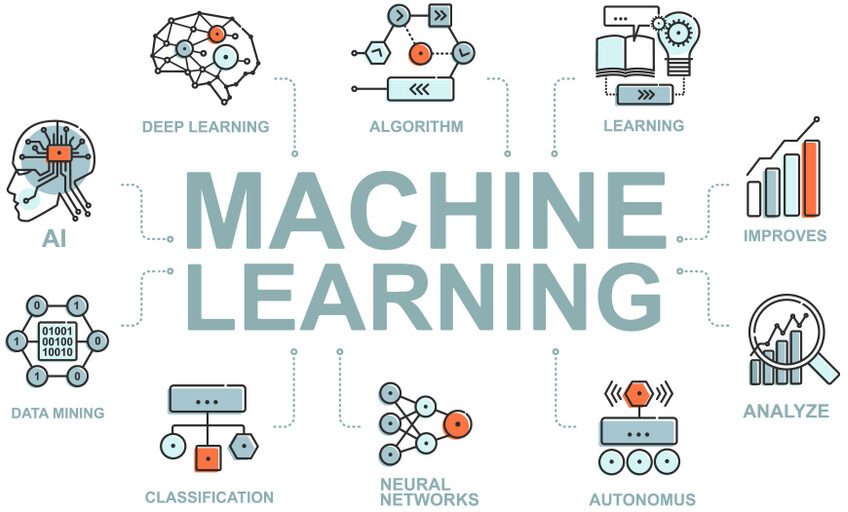
\includegraphics[height=2.3in,width=3.8in,viewport=0 0 630 390,clip]{Figures/Machine_Learning.jpg}
%\caption{\fontsize{7.2pt}{4.2pt}\selectfont{\textrm{人工智能与机器学习和深度学习的层次关系示意图.引自文献\cite{JPM2-032001_2019}}}}%
\label{Machine-Learning}
\end{figure}
\textcolor{blue}{用已知的数据关系预测未知数据或辅助不确定条件下的决策过程}
}

\frame
{
	\frametitle{人工智能\textrm{(Artificial Intelligence, AI)}与机器学习}
		获取材料完整物性数据的成本,无论是通过实验手段还是计算模拟,代价都是比较高
		\begin{itemize}
			\item 高通量第一原理计算自动流程和数据库解决了材料物性数据的获取问题%,但是并未给出现有材料数据基础上的物性优化的方案
			\item 利用数据挖掘技术,实现数据驱动的材料物性筛选、预测和提升的技术路线,有着特殊重要的意义
		\end{itemize}
	\vskip 8pt
	{\fontsize{8.2pt}{6.2pt}\selectfont{任何计算机模拟人类智能的算法都可以划归为人工智能,并非一定要应用机器学习算法,也包括决策树、知识库、计算机逻辑等算法
		\vskip 3pt
		{\fontsize{6.8pt}{4.2pt}\selectfont{\textcolor{blue}{人工智能广泛应用于金融、导航控制、语言处理、游戏竞技、计算机可视化和生物信息学等领域}}}
	\begin{itemize}
		\item 机器学习技术可以从大量数据中获得有价值的信息,尤其是面对高维复杂数据时,机器学习技术是确定数据间关系的有力的工具
	\item 机器学习领域的深度学习\textrm{(Deep Learning, DL)}是仿照生物神经网络\footnote{\fontsize{7.2pt}{6.2pt}\selectfont{神经网络结构意味着输入输出之间允许有多个类似神经的网络层}}结构为主要代表的一种示类学习
\end{itemize}}}
}

\frame
{
	\frametitle{人工智能和机器学习的层次关系}
	传统定义界定的机器学习,是指无须借助解析程序,直接依靠数据来提升任务处理的性能,自从\textrm{1950}年代统计学、计算科学与技术和神经科学的发展,机器学习的研究发展到了更广泛的人工智能领域%图\ref{AI-ML}表明了人工智能和机器学习的层次关系。
\begin{figure}[h!]
\centering
\vspace*{-0.1in}
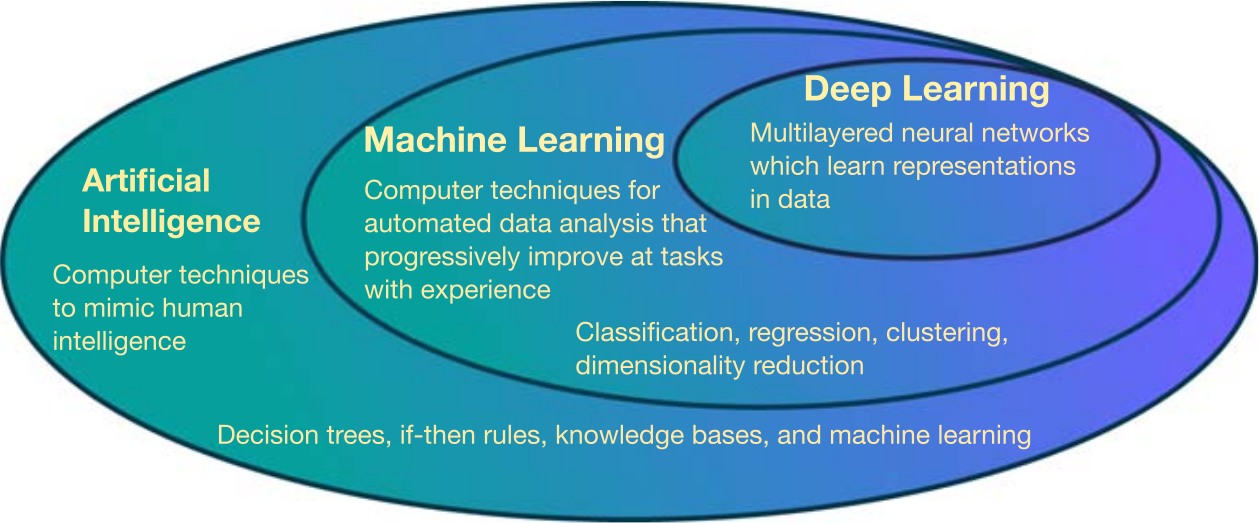
\includegraphics[height=1.9in,width=4.0in,viewport=0 0 1275 550,clip]{Figures/Hierarchical_description_AI_ML_DL.png}
\caption{\tiny{\textrm{Artificial Intelligence, Machine Learning and Deep Learning.}}}%
\label{AI-ML}
\end{figure}
}

\frame
{
	\frametitle{机器学习问题的一般形式与分类}
	\begin{itemize}
		\item 机器学习类问题的一般表示:
\vskip 5pt
对于给定的集合$\mathbf{X}$,可以预测或近似得到未知函数$y=f(\mathbf{X})$
\vskip 4pt
{\fontsize{6.2pt}{4.2pt}\selectfont{
	集合$\mathbf{X}$构成特征空间,集合中的每个元素$\mathbf{x}$称为特征向量(在材料类的机器学习中也称描述符)\\
	根据机器学习得到的近似函数$\hat{y}=\hat{f}(\mathbf{X})$,模型有能力预测训练数据之外的输出值}}
\vskip 5pt
	\textcolor{blue}{\fontsize{8.0pt}{4.2pt}\selectfont{机器学习的这种预测能力也称为模型的“泛化”\textrm{(generalization)}}}
\item 机器学习主要根据学习的特征分为无监督学习\textrm{(unsupervised learning)}和监督学习\textrm{(supervised learning)}
	\item 此外的机器学习问题还包括:~
\begin{itemize}
	\item 半监督学习,即大部分没有映射关系的数据和少量有映射关系的数据;
	\item 多任务和迁移学习,即将从相关问题习得的知识应用到数据极少的对象,提升模型的学习能力
	\item 强化学习,即没有输入输出,但会和环境不断交互,通过最大化环境的反馈,最终达到学习目标
\end{itemize}
	\end{itemize}
}

\frame
{
	\frametitle{机器学习问题的一般形式与分类}
\begin{figure}[h!]
\centering
\vspace*{-7pt}
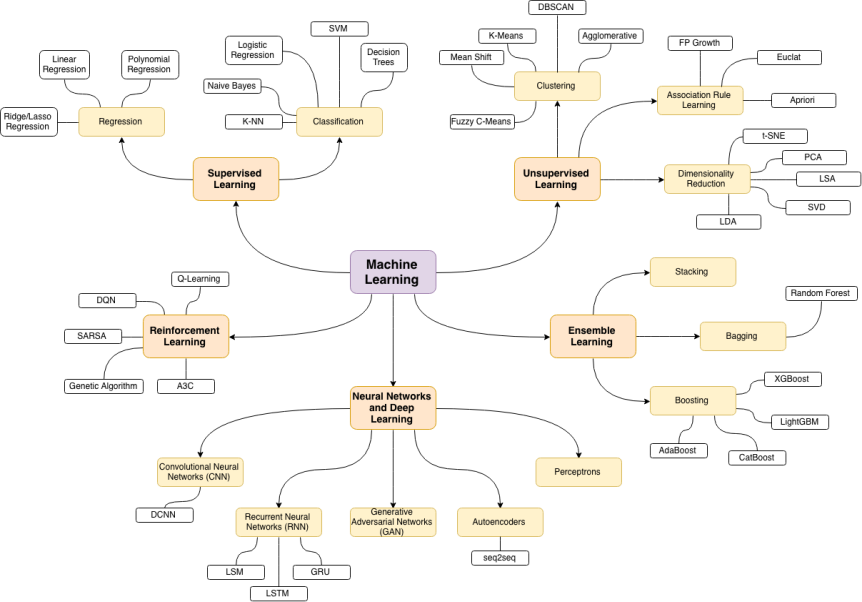
\includegraphics[height=2.7in,width=4.0in,viewport=0 0 875 620,clip]{Figures/ML_class.png}
%\caption{\fontsize{6.5pt}{4.5pt}\selectfont{面向多尺度材料智能计算平台}}%
\label{ML_classification}
\end{figure}
}

\frame
{
	\frametitle{数据挖掘的基本决策}
\begin{itemize}
	\item \textcolor{blue}{聚类}:~无指导的学习
	\item \textcolor{blue}{分类}:~有指导的学习
\end{itemize}
分类是数据挖掘的重要任务
\vskip 2pt
分类的\textcolor{red}{目的}:~机器学会分类函数或分类模型(称为分类器),通过模型能将数据库中的数据映射到特定类别中的某一类

\begin{figure}[h!]
\centering
\vspace*{-7pt}
\animategraphics[autoplay, loop, width=4.05in, height=1.55in]{15}{Figures/DNN-}{0}{15}
%\caption{\fontsize{6.5pt}{4.5pt}\selectfont{面向多尺度材料智能计算平台}}%
\label{ML_classification-animate}
\end{figure}
}

\frame
{
	\frametitle{无监督学习}
无监督学习是描述性质的,所有数据只有特征向量,没有标签,但呈现出聚群的结构,相似类型或特征的数据会聚集在一起
\begin{itemize}
	\item 如果没有标签的数据的组合是有限个,称为聚类\textrm{(clustering)};~无限的称为密度估计\textrm{(density estimation)}
	\item 将高维数据投影到低维空间,称为降维\textrm{(dimensionality reduction)}
		\vskip 2pt
		{\fontsize{8.0pt}{4.2pt}\selectfont{降维有助于了解复杂数数据的检测模式}}
%	\item 识别数据中的异常点或离群点
%		\vskip 2pt
%		{\fontsize{8.0pt}{4.2pt}\selectfont{异常检测可用于欺诈检测、故障预警等场景}}
\end{itemize}
\begin{figure}[h!]
\centering
\vspace*{-0.1in}
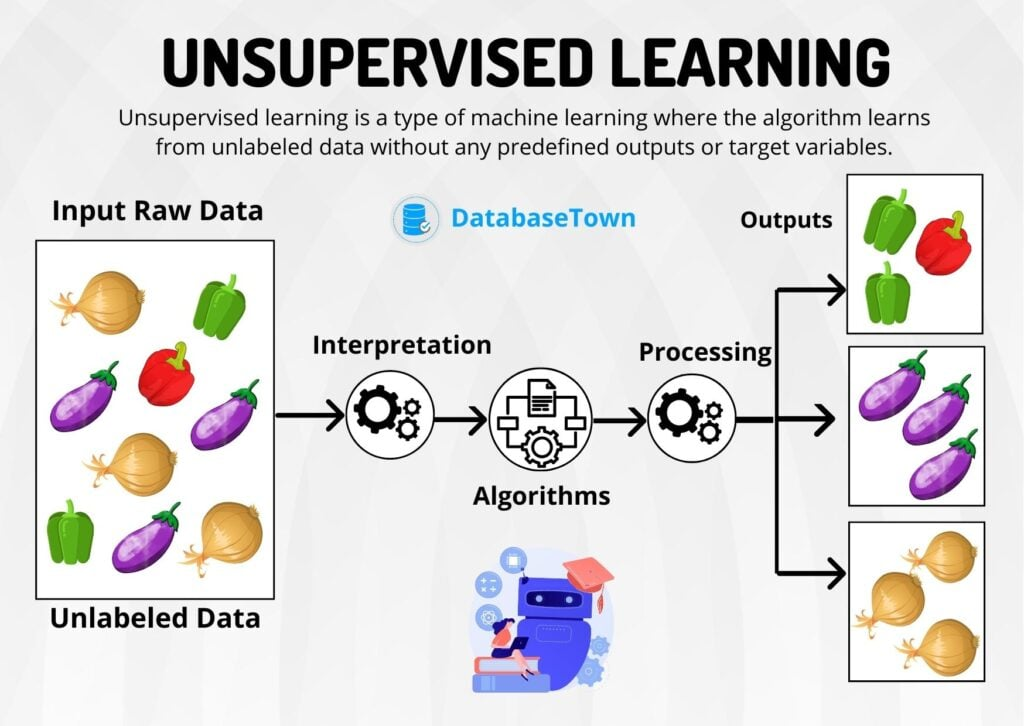
\includegraphics[height=1.5in,width=2.7in,viewport=0 0 1075 720,clip]{Figures/ML_Unsupervised-Learning.jpg}
\caption{\tiny{\textrm{The Schematic diagram of Unsupervised Learning.}}}%
\label{ML_Unsupervised-Learning}
\end{figure}
}

\frame
{
	\frametitle{监督学习}
	监督学习是通过学习指定数量的输入输出间的函数映射
\begin{itemize}
	\item 如果输出函数$y_{\mathrm{i}}$表示类别的有限集合,称为分类\textrm{(classification)}问题
		\vskip 2pt
		{\fontsize{8.0pt}{4.2pt}\selectfont{模型可用来预测未知数据所属类型}}
	\item 如果输出函数$y$是实数,称为回归\textrm{(regression)}问题
		\vskip 2pt
		{\fontsize{8.0pt}{4.2pt}\selectfont{模型可用来预测未知输入数据对应的值输出值}}
\end{itemize}
\begin{figure}[h!]
\centering
\vspace*{-0.1in}
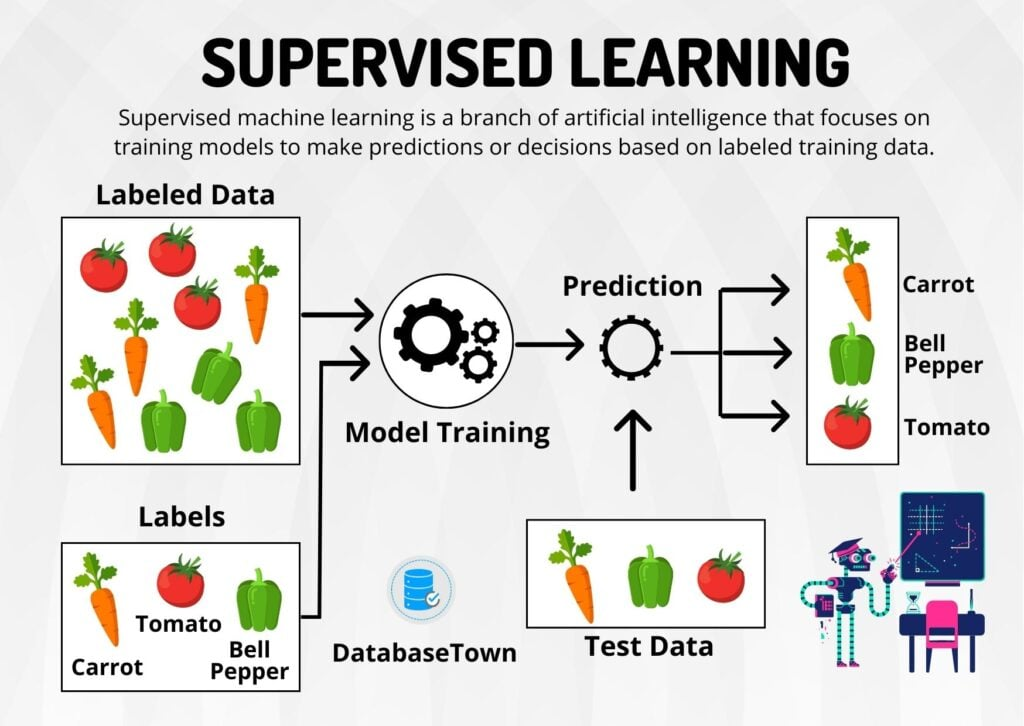
\includegraphics[height=1.6in,width=2.8in,viewport=0 0 1075 720,clip]{Figures/ML_Supervised-Learning-2.jpg}
\caption{\tiny\selectfont{\textrm{The Schematic diagram of Supervised Learning.}}}%
\label{ML_Supervised-Learning}
\end{figure}
}

\frame
{
	\frametitle{机器学习的流程}
\begin{itemize}
	\item \textcolor{blue}{数据的收集和筛选}:~{\fontsize{8.0pt}{4.2pt}\selectfont{从现有数据中产生并选择与问题解决有用和相关的数据子集}}
	\item \textcolor{blue}{数据预处理}:~清洗缺失和不完整数据,将数据将转换成统一的格式{\fontsize{8.0pt}{4.2pt}\selectfont{(如整型、字符串型等)}}%。必要时还须根据需要将数据按问题的格式重新表示
	\item \textcolor{blue}{数据训练}:~将数据分为训练集、验证集和测试集三部分,训练集数据用于学习并得到模拟参数{\fontsize{8.0pt}{4.2pt}\selectfont{(主要针对监督学习)}}
	\item \textcolor{blue}{模型测试和优化}:~用验证集数据评估模型的效果和性能,并用验证集数据优化模型
		\vskip 3pt
		{\fontsize{8.0pt}{4.2pt}\selectfont{一旦完成优化,用测试集数据评定模型的性能}}%。如果学习不成功,选用改善的数据重复上述步骤或改变学习算法。
	\item \textcolor{blue}{模型应用}:~将得到的有效模型对未知数据进行预测,如果有新的数据,模型还可以继续训练
\end{itemize}
}

\section{机器学习算法}
\frame
{
	\frametitle{主成分分析\textrm{(principal component analysis)}}
	主成分分析:\\
	{\fontsize{8.0pt}{4.2pt}\selectfont{\textcolor{blue}{将高维数据投影到数据点集中的区域,并使数据在新轴向周围聚集度最高}}}
{\fontsize{8.0pt}{4.2pt}\selectfont{
	\begin{itemize}
		\item 确定主成分:~找到$\mathbf{X}^T\mathbf{X}$的最大本征值对应的本征矢量(称为主成分)
			\vskip 1.5pt
			{\fontsize{7.0pt}{4.2pt}\selectfont{$\mathbf{X}$是已知高维数据集构成的矩阵}}
		\item 数据投影:~计算所有数据点对主成分的投影,实现数据压缩
		\item 局限:~ 假设数据位于线性子空间中
			\vskip 1.5pt
			{\fontsize{7.0pt}{4.2pt}\selectfont{只能为线性数据提供最佳结果}}
	\end{itemize}}}
\begin{figure}[h!]
\centering
\vspace*{-0.1in}
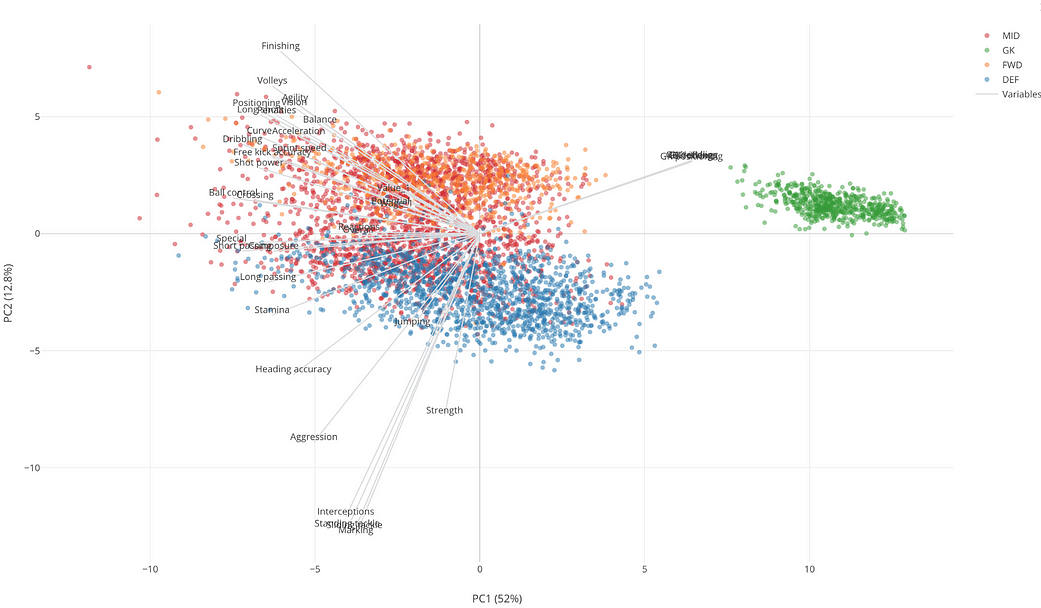
\includegraphics[height=1.70in,width=2.9in,viewport=0 0 1040 620,clip]{Figures/ML_PCM.png}
\caption{\tiny{\textrm{The Schematic diagram of Principal component analysis.}}}%
\label{ML_PCM}
\end{figure}
}

\frame
{
	\frametitle{$k$-\textrm{means}算法}
	$k$-\textrm{means}算法:~{\fontsize{8.0pt}{4.2pt}\selectfont{\textcolor{blue}{直接计算数据点和聚类中心的欧氏距离\textrm{(Euclidean distance)},将$n$个数据分类为$k$个子集($k<n$)}}}
	\vskip 3pt
{\fontsize{8.0pt}{4.2pt}\selectfont{
随机选定聚类中心的个数($k$)和位置($\mathbf{\mu}_0^{(\mathrm{j})}$,$1\leqslant j \leqslant k$),执行迭代:~
\begin{itemize}
	\item 计算每个数据点与聚类中心的距离,标记为$y_t^{\mathrm{(i)}}~(t>0)$,将该点分到距离最小的聚类中心所属的类中
		\begin{displaymath}
			y_t^{(\mathrm{i})}=\textrm{argmin}_j\|\mathbf{x}^{(\mathrm{i})}-\mu_t^{(\mathrm{j})}\|_p
		\end{displaymath}
	\item 重新计算每个聚类的中心$(\{\mu_t^{(\mathrm{j})}\})$
		\begin{displaymath}
			\mu_{t+1}^{(\mathrm{j})}=\dfrac1{n_j}\sum_{i=1}^{n_j}\mathbf{x}^{(\mathrm{i})}\delta_{y_t^{(\mathrm{i})},\mathrm{j}}
		\end{displaymath}
		$p\in\mathbb{N}$表示空间的维度(当$p=2$即为是二维平面的欧氏距离),$n_j$是归入聚类中心$\mu_t^{(\mathrm{j})}$的分类元素数目,$\delta_{n,m}$表示$\Delta$函数,$t$表示迭代次数
\end{itemize}
当标记不再变化时,迭代收敛}}
}

\frame
{
	\frametitle{$k$-\textrm{means}算法}
\begin{figure}[h!]
\centering
\vspace*{-0.1in}
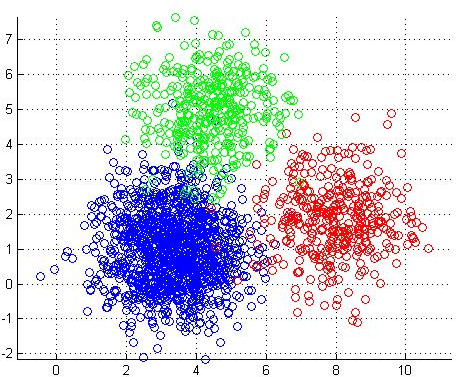
\includegraphics[height=1.80in,width=2.2in,viewport=0 0 110 90,clip]{Figures/ML_k-mean.png}
\caption{\tiny{\textrm{The Schematic diagram of the $k$-means algorithm.}}}%
\label{ML_k-means}
\end{figure}
$k$-\textrm{means}聚类算法的结果与初始聚类中心位置的选择密切关联
\vskip 3pt
{\fontsize{8.0pt}{4.2pt}\selectfont{初始聚类中心选择得不同,结果差别会比较大\footnote{\fontsize{6.0pt}{4.2pt}\selectfont{一般克服的策略是通过多次初始聚类中心并执行该算法,选择最有代表性的聚类形式作为结果}}}}
}

\frame
{
	\frametitle{层次聚类\textrm{(Hierarchical Clustering)}算法}
	层次聚类:~{\fontsize{8.0pt}{4.2pt}\selectfont{\textcolor{blue}{通过一层一层的进行聚类}}}
	\vskip 2pt
	{\fontsize{7.0pt}{4.2pt}\selectfont{\textcolor{magenta}{分裂法}:~由上向下把大的类别分割\\
	\textcolor{magenta}{聚合法}:~由下向上对小的类别聚合}}
{\fontsize{7.0pt}{4.2pt}\selectfont{
\begin{itemize}
	\item 初始时将每个训练数据点$\mathbf{x}^{(\mathrm{i})}$作为一个类(或类簇),原始类大小等于训练数据点数目$n$
	\item 衡量任意两个类(分别标记为\textrm{A}和\textrm{B})的偏差$d(\mathrm{A},\mathrm{B})$
	\item 偏差最小的两个类(最相似)合并一个新的类簇
\end{itemize}
反复执行该聚合过程,最终可以用一个类簇能囊括全部训练集}}
\begin{figure}[h!]
\centering
\vspace*{-0.04in}
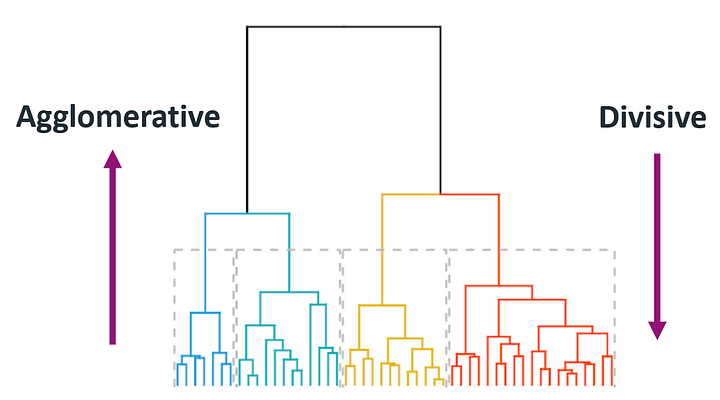
\includegraphics[height=1.47in,width=3.2in,viewport=0 0 730 390,clip]{Figures/ML_Hierarchical-Clustering.png}
\caption{\tiny{\textrm{The Schematic diagram of Hierarchical-Clustering algorithm.}}}%
\label{ML_ML_Hierarchical-Clustering}
\end{figure}
}

\frame
{
	\frametitle{层次聚类\textrm{(Hierarchical Clustering)}算法}
{\fontsize{8.0pt}{4.2pt}\selectfont{
要将$n$个类聚合成$k$个类簇~($1<k<n$)~,要在聚合中对聚合偏差设置截断,常见的聚合截断有三种:
\begin{itemize}
	\item 最小偏差
\begin{displaymath}
	d_{\mathrm{SL}}(\mathrm{A},\mathrm{B})=\min\limits_{i\in\mathrm{A},j\in\mathrm{B}}d_{ij}
\end{displaymath}
$d_{ij}$表示任意一对类的偏差
	\item 最大偏差
\begin{displaymath}
	d_{\mathrm{CL}}(\mathrm{A},\mathrm{B})=\max\limits_{i\in\mathrm{A},j\in\mathrm{B}}d_{ij}
\end{displaymath}
	\item 平均偏差
\begin{displaymath}
	d_{\mathrm{GA}}(\mathrm{A},\mathrm{B})=\dfrac1{|\mathrm{A}||\mathrm{B}|}\sum\limits_{i\in\mathrm{A}}\sum\limits_{j\in\mathrm{B}}d_{ij}
\end{displaymath}
\end{itemize}
定义的$d_{ij}$可以人为指定,对数值形式的数据,最常见的设置为欧氏距离}}
\vskip 5pt
分裂法与聚合法类似,只是初始时训练数据集属于一个类簇,然后逐层分裂形成特定的类簇
}

\frame
{
	\frametitle{线性回归\textrm{(Linear Regression)}算法}
对监督学习来说,每个数据不仅有特征向量$\mathbf{x}_{\mathrm{i}}$,还有相应的值$y_{\mathrm{i}}$
预测连续变化的$y$值,最常用的算法是线性回归
\vskip 3pt
{\fontsize{8.0pt}{4.2pt}\selectfont{回归算法的基本思想:~\textcolor{blue}{对于满足正态分布的数据点}
	\begin{itemize}
			\item 允许的参数拟合预测表达式
\begin{displaymath}
	\hat y^{(\mathrm{i})}=\theta^T\mathbf{x}^{(\mathrm{i})}
\end{displaymath}
{\fontsize{6.0pt}{4.2pt}\selectfont{上标$T$表示矢量的转置,$\hat y^{(\mathrm{i})}$是预测值,$\theta$是参数的矢量}}
		\item 为了求得$\theta$参数,定义误差的最小二乘函数
\begin{displaymath}
	J(\theta)=\sum_{i=1}^nL[\hat{y}^{(\mathrm{i})}(\mathbf{x}^{(\mathrm{i})},\theta),y^{(\mathrm{i})}]=\dfrac12\sum_{i=1}^n(\theta^T\mathbf{x}^{(\mathrm{i})}-y^{(\mathrm{i})})^2
\end{displaymath}
{\fontsize{6.0pt}{4.2pt}\selectfont{最小化该函数,可以得到最优化的参数$\theta$,由此可以得到线性回归机器学习的模型}}
\item 最优化参数$\theta$用矩阵表示可写作:~
\begin{displaymath}
	\theta=(\mathbf{X}^T\mathbf{X})^{-1}\mathbf{X}^T\mathbf{y}
\end{displaymath}
{\fontsize{6.0pt}{4.2pt}\selectfont{这里$\mathbf{X}$矩阵的每一列是由训练集输入数据$\mathbf{x}^{(\mathrm{i})}$,$\mathbf{y}$是对应的输出标注构成的矢量}}
	\end{itemize} }}
}

\frame
{
	\frametitle{预测模型的检验}
机器学习的模型性能,可用测试数据集检验,预测误差与训练数据集包含的数据数量密切相关:
\begin{itemize}
	\item 训练集数据不够,模型不能完全反映训练集特征\\
		{\fontsize{8.0pt}{4.2pt}\selectfont{预测结果将会表现出明显的偏差}}
	\item 训练集数据过多,模型能够体现训练集特征\\
		{\fontsize{8.0pt}{4.2pt}\selectfont{对训练集外的数据效果不好,出现过拟合\textrm{(overfitting)}}}
\end{itemize}
\begin{figure}[h!]
\centering
\vspace*{-0.1in}
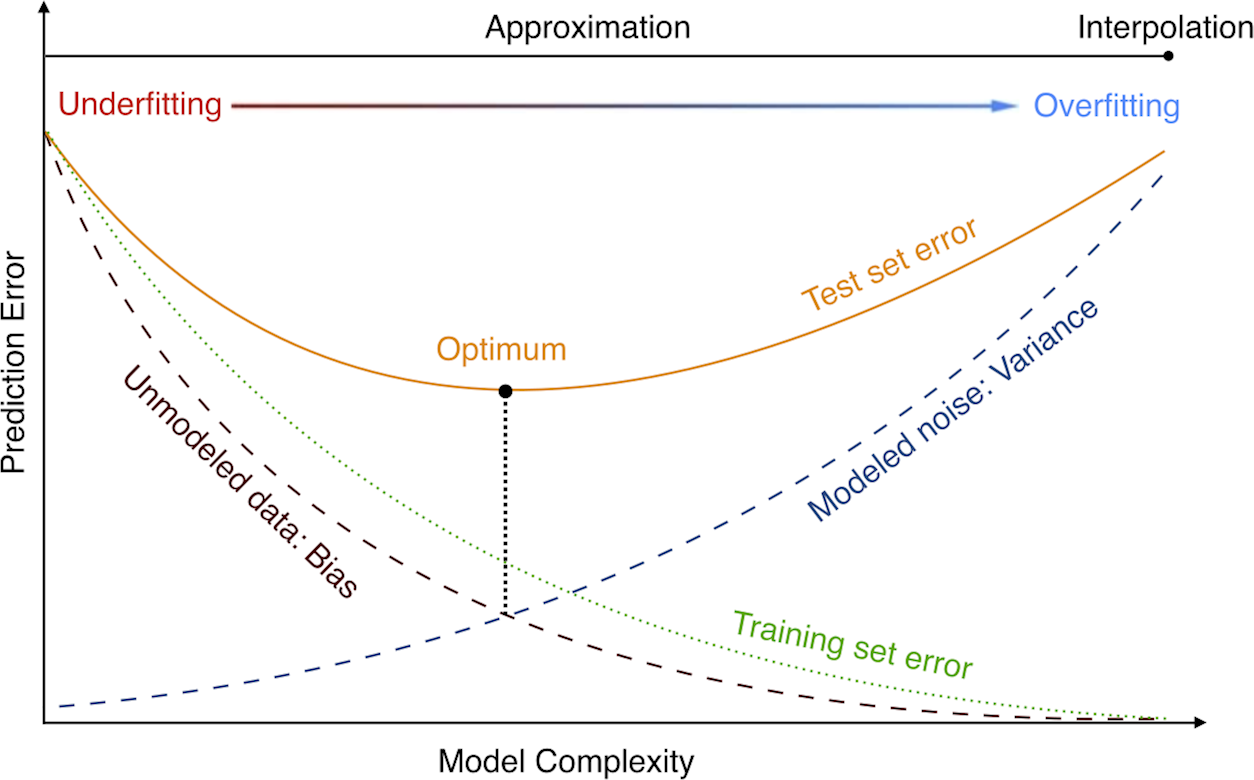
\includegraphics[height=1.4in]{The_optimum_comlexity_vs_prediction.png}
\caption{\tiny{\textrm{Complexity of the model:~Effective number of degrees of freedom (mainly tuned by the hyperparameters of the estimator).}}}%
\label{ML_Fitting_Error}
\end{figure}
}

\frame
{
	\frametitle{预测模型的检验}
回归算法的发展:~构建模型时,通过引入标准化参数$\lambda$来反应训练集元素变化的影响
\begin{displaymath}
	J(\theta)=\dfrac12\sum_{i=1}^n(\theta^T\mathbf{x}^{(\mathrm{i})}-y^{(\mathrm{i})})^2+\lambda\|\theta\|_p
\end{displaymath}
{\fontsize{7.0pt}{4.2pt}\selectfont{这里$p$表示数据度量形式}}
\vskip 4pt
{\fontsize{8.0pt}{4.2pt}\selectfont{优化参数$\lambda$降低训练集数据数量的影响:
	\vskip 3pt
	\textcolor{magenta}{通过压制或筛选训练数据集中的特征来调节其对误差函数的贡献}
\begin{itemize}
	\item $p=1$:~\textrm{Ridge Regression}
	\item $p=2$:~\textrm{LASSO Regression} 
\end{itemize}
\vskip 4pt
注意:~$\lambda$不能像$\theta$一样被优化}}
\vskip 2pt
{\fontsize{6.0pt}{4.2pt}\selectfont{一般是通过比较几个不同的$\lambda$值,选其中能最大化预测能力又不会引入太大偏差的一个}}
}

\frame
{
	\frametitle{分类算法:~逻辑回归\textrm{(logistic regression)}}
	逻辑回归,{\fontsize{8.0pt}{4.2pt}\selectfont{\textcolor{blue}{可以类比为映射到区间$[0,1]$之间的线性回归}}}: 
	\vskip 2pt
\begin{minipage}[b]{0.55\textwidth}
{\fontsize{7.0pt}{4.2pt}\selectfont{对于给定数据点$\mathbf{x}^{(i)}$,
\begin{itemize}
	\item $y^{(i)}=1$:~将其分入特定的“是\textrm{(True)}”类
	\item $y^{(i)}=0$:~将其分入特定的“否\textrm{(False)}”类
\end{itemize}
预测函数可以表示为
\begin{displaymath}
	\hat y=\sigma(\theta^T\mathbf{x})=\dfrac1{1+\mathrm{e}^{-\theta^T\mathbf{x}}}
\end{displaymath}
{\fontsize{5.0pt}{4.2pt}\selectfont{这里$\theta$仍是参数矢量,$\sigma$是逻辑函数(或 \textrm{sigmoid}函数)}}
\vskip 2pt
预测函数也可以视为条件概率:~$\hat{y}=P(y=1|\mathbf{x},\theta)$}}
\end{minipage}
\hfill
\begin{minipage}[b]{0.43\textwidth}
\begin{figure}[h!]
\centering
\vspace*{-0.4in}
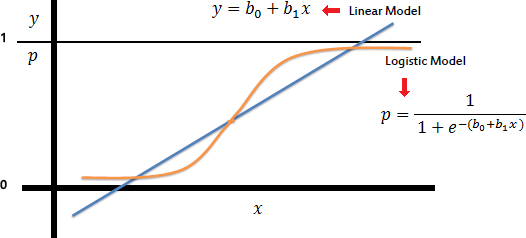
\includegraphics[height=0.75in]{ML_LR-LogReg.png}
%\caption{\tiny{\textrm{The Schematic diagram of linear model vs logistic model.}}}%
\label{ML_LR-LogReg}
\end{figure}
\end{minipage}
\vskip 2pt
{\fontsize{6.0pt}{4.2pt}\selectfont{分类问题的误差函数可定义为负的$\log$-型函数(交互熵\textrm{cross-entropy}),同样通过参数$\theta$最小化该函数:
\begin{displaymath}
	J(\theta) = -\dfrac1n\sum_{i=1}^n[y^{(\mathrm{i})}\log(\hat{y}^{(\mathrm{i})})+(1-y^{(\mathrm{i})})\log(1-\hat{y}^{(\mathrm{i})})]
\end{displaymath}
{\fontsize{5.0pt}{4.2pt}\selectfont{这里$y^{(\mathrm{i})}$和$\hat{y}^{(\mathrm{i})}=\sigma(\theta^T\mathbf{x}^{(\mathrm{i})})$分别为实际和预测值}}
\vskip 1pt
和线性回归类似,也可以引入正则参数$\lambda$}}
\vskip 2pt
{\fontsize{7.0pt}{4.2pt}\selectfont{逻辑分类也可用于处理超过两类的数据分类:\\
%	\vskip 1pt
	\textcolor{blue}{训练有$n$个逻辑回归值的模型,每一类对应一个数值,每个数据分入概率值最高的类中}}}
}

\frame
{
	\frametitle{支持向量机\textrm{(Support Vector Machines)}}
	支持向量机:~{\fontsize{7.5pt}{4.2pt}\selectfont{\textcolor{blue}{最通用的分类算法}
\vskip 2pt
定义函数
\begin{displaymath}
	J(\theta)=C\sum_{i=1}^n[y^{(\mathrm{i})}\max(\theta^T\mathbf{x}^{(\mathrm{i})},0)+(1-y^{(\mathrm{i})})\max(-\theta^T\mathbf{x}^{(\mathrm{i})},0)]+\dfrac1n\sum_{i=1}^n\theta_i^2
\end{displaymath}
{\fontsize{6.0pt}{4.2pt}\selectfont{这里$C$是参数}}
\begin{itemize}
	\item 在约束条件$y^{(\mathrm{i})}(\theta^T\mathbf{x}^{(\mathrm{i})}+b)\leqslant1$下,对全部训练数据点$(\mathbf{x}^{(\mathrm{i})},y^{(\mathrm{i})})$实现$\|\theta\|^2$最小化
	\item 引入\textrm{Lagrangian}乘子最小化$\|\theta\|^2$,可根据测试数据$i$的值$y^{(\mathrm{i})}$($+1$或$-1$),确定数据所属的类
\end{itemize}}}
\begin{figure}[h!]
\centering
\vspace*{-0.1in}
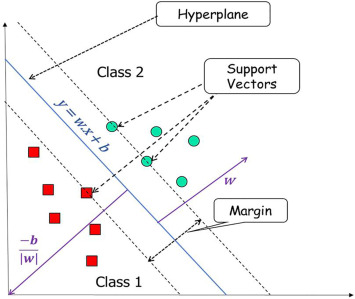
\includegraphics[height=1.4in,width=1.6in,viewport=0 0 230 190,clip]{ML_SVM.jpg}
\caption{\tiny{\textrm{The Schematic diagram of support vector machines algorithm.}}}%
\label{ML_SVM}
\end{figure}
}

\frame
{
	\frametitle{支持向量机\textrm{(Support Vector Machines)}}
	{\fontsize{7.5pt}{4.2pt}\selectfont{\textcolor{blue}{\textrm{SVM}最重要的特色是内核技巧\textrm{(kernel trick)}}\\
将参数矢量$\theta$用训练集数据表示
\begin{displaymath}
	\theta=\sum_i\alpha_iy^{(\mathrm{i})}\mathbf{x}^{(\mathrm{i})}
\end{displaymath}
因此可将分类规则写成数据点积的形式
\begin{displaymath}
	\theta^T\mathbf{x}+b=\sum_i\alpha_iy^{(\mathrm{i})}\mathbf{x}^{(\mathrm{i})}\cdot\mathbf{x}+b\leqslant0\rightarrow y=+1
\end{displaymath}
{\fontsize{6.0pt}{4.2pt}\selectfont{这里$b$和$\{\alpha_i\}$是待学习的参数}}
\vskip 2pt
\textcolor{blue}{内核技巧利用映射关系$\phi(\mathbf{x}):~\mathtt{R}^n\rightarrow\mathtt{R}^m$将矢量变换成$\mathbf{x}^{(\mathrm{i})}\cdot\mathbf{x}$点积}
\vskip 1pt
{\fontsize{6.0pt}{4.2pt}\selectfont{\textcolor{cyan}{实际上是将数据点映射到更高维度的空间中}}}
\vskip 2pt
所有矢量点积映射的变换都可以类似处理,最常用的内核
\begin{itemize}
	\item 多项式内核:
\begin{displaymath}
	K(\mathbf{x}^{(\mathrm{i})},\mathbf{x}^{(\mathrm{j})})=\phi(\mathbf{x}^{(\mathrm{i})})\cdot\phi(\mathbf{x}^{(\mathrm{j})})=(\mathbf{x}^{(\mathrm{i})}\cdot\mathbf{x}^{(\mathrm{j})}+1)^d,~d\in\mathtt{N}
\end{displaymath}
\item \textrm{Gaussian}内核(\textrm{radial basis function, RBF}内核)
\begin{displaymath}
	K(\mathbf{x}^{(\mathrm{i})},\mathbf{x}^{(\mathrm{j})})=\mathrm{e}^{\dfrac{-\|\mathbf{x}^{(\mathrm{i})},\mathbf{x}^{(\mathrm{j})}\|^2}{2\sigma^2}}
\end{displaymath}
\end{itemize}}}
}

\frame
{
	\frametitle{\textrm{Na\"ive~Bayes}分类}
{\fontsize{8.0pt}{4.2pt}\selectfont{
分类算法的判别模式
\begin{itemize}
	\item 基于判别模式\textrm{(discriminative model)}:~数据点预测的标签是条件概率$p(y|\mathbf{x})$
	\item 基于生成模式\textrm{(generative model)},预测点条件概率用后验\textrm{Bayes}公式表示
\begin{displaymath}
	p(y|\mathbf{x})=\dfrac{p(\mathbf{x}|y)p(y)}{p(\mathbf{x})}=\dfrac{p(\mathbf{x}|y)p(y)}{\sum\limits_ip(\mathbf{x}|y=i)p(y=i)}
\end{displaymath}
{\fontsize{6.0pt}{4.2pt}\selectfont{这里$p(y)$表示先验概率,即没有附加任何先期知识和分析得到的概率}}
\end{itemize}
\begin{minipage}[b]{0.59\textwidth}
假设数据点的特征向量$\mathbf{x}^{(\mathrm{i})}$和值$y^{(\mathrm{i})}$完全独立,可有\textrm{Na\"ive~Bayes}分类算法(后验概率):
\begin{displaymath}
	p(y|\mathbf{x})=\dfrac{\prod\limits_{j=1}^np(x_j|y)p(y)}{p(\mathbf{x})}
\end{displaymath}
{\fontsize{6.0pt}{4.2pt}\selectfont{这里$x_j$表示特征向量$\mathbf{x}$的元素}}%,这里主要讨论分子,因为分母先验概率$p(\mathbf{x})$是与$y$无关的常数且和是归一化的
\end{minipage}
\hfill
\begin{minipage}[b]{0.39\textwidth}
\begin{figure}[h!]
\centering
\vspace*{-0.05in}
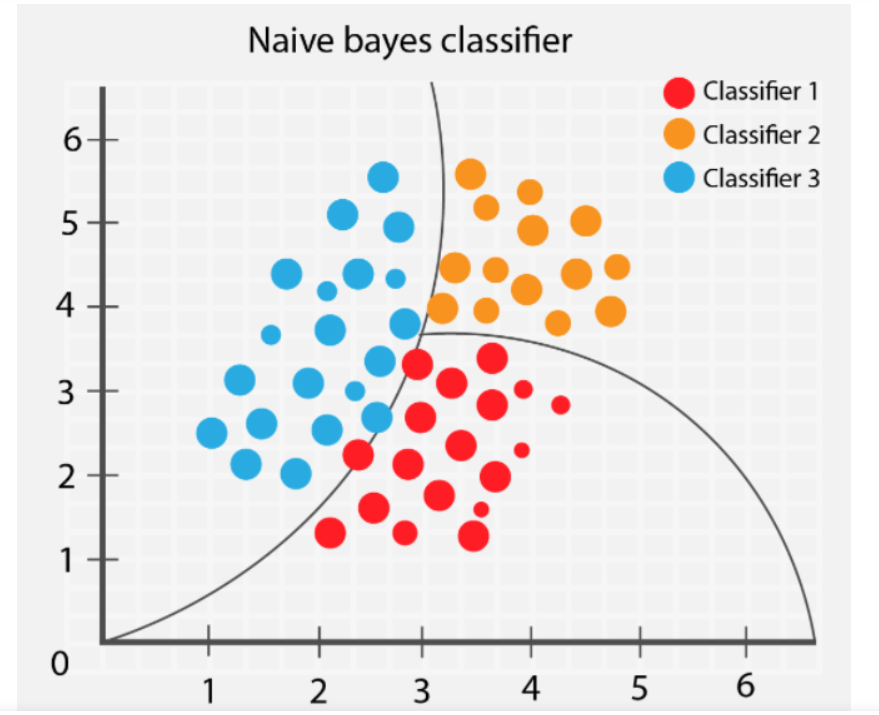
\includegraphics[height=1.2in,width=1.5in,viewport=0 0 550 470,clip]{ML_Naive-Bayes.png}
%\caption{\tiny{\textrm{The Schematic diagram of Na\"ive-Bayes algorithm.}}}%
\label{ML_NavieBayes}
\end{figure}
\end{minipage}
\begin{itemize}
	\item 分类前先列出训练数据点的全部先验概率$p(y)$和条件概率$p(x_j|y)$
	\item 用\textrm{Na\"ive~Bayes}算法计算后验概率
	\item 选择所有$y$中最大的后验概率$p(y|\mathbf{x})$作为分类预测值
\end{itemize}}}
}

\frame
{
	\frametitle{$k$-最近邻\textrm{($k$-nearest neighbors)}算法}
	$k$-最近邻算法:~{\fontsize{8.0pt}{4.2pt}\selectfont{\textcolor{blue}{利用数据点空间距离的类似性,不再训练,适合处理快速任务}
\vskip 3pt
	$d$-维空间有训练集数据$\{\mathbf{x}^{(\mathrm{i})}\}$,计算未知数据点与已知数据点之间的空间距离
\begin{displaymath}
	d(\mathbf{x},\mathbf{x}^{(\mathrm{i})})=\|\mathbf{x}-\mathbf{x}^{(\mathrm{i})}\|_p
\end{displaymath}
{\fontsize{6.0pt}{4.2pt}\selectfont{这里的$p$是维度参数}}
\vskip 3pt
一旦得到$\mathbf{x}$到空间各点的距离,$\mathbf{x}$点归入与其有最近邻$k$值最大的类中
\vskip 2pt
如果没有最大类,则随机归入最近邻点的最常使用的标注类中
\begin{itemize}
	\item 对连续值求平均,就是基于\textrm{k-NN}的回归
	\item $k$值的选取对于分类很敏感,不同的$k$值很可能得到完全不同的数据分类
\end{itemize}}}
\begin{figure}[h!]
\centering
\vspace*{-0.1in}
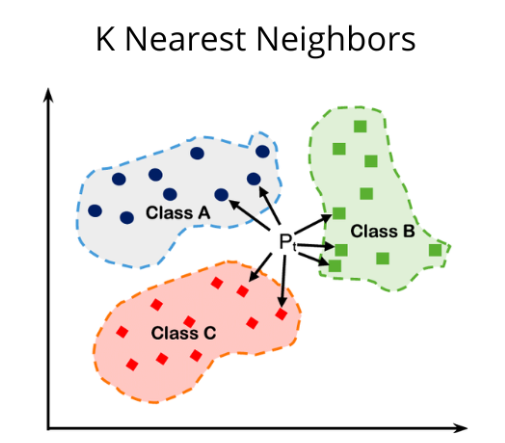
\includegraphics[height=1.5in,width=1.8in,viewport=0 0 530 450,clip]{ML_kNN-2.png}
\caption{\tiny{\textrm{The Schematic diagram of $k$-nearest neighbors algorithm.}}}%
\label{ML_k-NN}
\end{figure}
}

\frame
{
	\frametitle{决策树\textrm{(Decision Trees)}}
	决策树:~{\fontsize{8.0pt}{4.2pt}\selectfont{\textcolor{blue}{通过创建节点来实现对某种分裂算法的优化}
	\vskip 2pt
	\textcolor{magenta}{同时适合分类和回归}
	\begin{itemize}
		\item 决策树上每个节点都含一个定义该部分空间划分的方案,直到空间不可再分
		\item 每个不连通的子空间称为\textcolor{blue}{叶节点},叶节点包含了待分类或预测的数据点
	\end{itemize}
决策树的主要问题:~一旦开始训练,往往伴随过拟合}}
\begin{figure}[h!]
\centering
%\vspace*{-0.05in}
\includegraphics[height=1.95in,width=3.4in,viewport=0 0 2070 1250,clip]{ML_decision-trees.png}
\caption{\tiny{\textrm{The Schematic diagram of decision trees algorithm.}}}%
\label{ML_Decision-trees}
\end{figure}
}

\frame
{
	\frametitle{随机森林\textrm{(Random Forest)}}
{\fontsize{8.0pt}{4.2pt}\selectfont{克服决策树过拟合的策略:
\begin{itemize}
	\item 修剪决策树分叉,会损失一定的精度,但提高回归的泛化能力
	\item 采用随机森林,即训练大量的决策树然后再取统计平均值
\end{itemize}
随机森林方法是一种系综平均方法:~\textcolor{blue}{决策树将成为训练对象}
\vskip 2pt
对决策树的特征进行随机抽样训练时,一般采取自展抽样\textrm{(bootstrap sample)}方案
\begin{figure}[h!]
\centering
%\vspace*{-0.05in}
\includegraphics[height=2.00in,width=3.0in,viewport=0 15 570 400,clip]{ML_radom-forest.png}
\caption{\tiny{\textrm{The Schematic diagram of random forest algorithm.}}}%
\label{ML_Random-Forest}
\end{figure}
随机森林算法将一系列的非强化学习的功能组合起来,对未知数据有更好的预测能力}}
}

\frame
{
	\frametitle{深度神经网络基础}
{\fontsize{8.0pt}{4.2pt}\selectfont{
	\begin{itemize}
		\item 感知机(\textrm{Perceptron Learning Algorithm, PLA}):
			\vskip 3pt
			最早的监督式训练算法,是神经网络构建的基础
\begin{figure}[h!]
%\vspace*{-0.08in}
\centering
\includegraphics[height=0.50in]{Figures/DNN_PLA.png}
\caption{\tiny \textrm{Perceptron Learning Algorithm.}}%(与文献\cite{EPJB33-47_2003}图1对比)
\label{Fig:PLA}
\end{figure}
输出与输入之间将学习到一个线性关系,可有中间输出结果
\begin{displaymath}
	z=\sum_{i=1}^mw_ix_i+b
\end{displaymath}
中间结果连接一个神经元激活函数
\begin{displaymath}
	\mathrm{sign}(z)=\left\{
		\begin{aligned}
			-1\qquad &z<0\\
			1 \qquad &z\geqslant 0
		\end{aligned}\right.
\end{displaymath}
	\end{itemize}}}
}

\frame
{
	\frametitle{深度神经网络基础}
\begin{figure}[h!]
\vspace*{-0.08in}
\centering
\includegraphics[width=2.5in]{Figures/NN_PLA_example.png}
%\caption{\tiny \textrm{Perceptron Learning Algorithm.}}%(与文献\cite{EPJB33-47_2003}图1对比)
\label{Fig:PLA}
\end{figure}
{\fontsize{8.0pt}{4.2pt}\selectfont{
\begin{itemize}
	\item 每一个输入数据都可以表示为一个向量$x = (x_1, x_2)$
	\item 函数则是要实现“如果线以下,输出0;线以上,输出1”
\end{itemize}}}
}

\frame
{
	\frametitle{深度神经网络基础}
{\fontsize{8.0pt}{4.2pt}\selectfont{
感知机模型只能用于二元分类,无法学习较为复杂的非线性模型,神经网络在感知机模型基础上作了扩展
%\vskip 10pt
	\begin{itemize}
		\item 加入隐藏层(\textrm{hide layer}):\\
			隐藏层可以有很多层,增强模型的表达能力
		\item 输出层的神经元可以有不止一个输出
		\item 对激活函数作扩展,如\textrm{Sigmoid}函数
			\begin{displaymath}
				f(z)=\dfrac1{1+\mathrm{e}^{-z}}
			\end{displaymath}
			{\fontsize{6.5pt}{4.2pt}\selectfont{其他的激活函数还有\textrm{tanx}、\textrm{softmax}和\textrm{ReLU}等}}
\begin{figure}[h!]
%\vspace*{-0.08in}
\centering
\includegraphics[width=2.8in]{Figures/ML_Sigmoid-Gjl-t.png}
%\caption{\tiny \textrm{Perceptron Learning Algorithm.}}%(与文献\cite{EPJB33-47_2003}图1对比)
\label{Fig:Sigmoid_curve}
\end{figure}
	\end{itemize}}}
}

\frame
{
	\frametitle{深度神经网络\textrm{(Deep Learning Neural Network)}}
{\fontsize{8.0pt}{4.2pt}\selectfont{
深度神经网络可以包含上百层神经元,通常有上万个参数,再加上超参数,实际的参数空间几乎是无限大的
\begin{figure}[h!]
%\vspace*{0.05in}
\centering
\includegraphics[height=1.90in,width=4.05in]{Figures/ANN_Algorithm.png}
\caption{\tiny \textrm{Deep Learning Neural Network.}}%(与文献\cite{EPJB33-47_2003}图1对比)
\label{Fig:Deep-Learning-NN}
\end{figure}
\textcolor{red}{如何从海量潜在的可能参数中做选择极具挑战性}}}
}

\frame
{
	\frametitle{深度神经网络的前馈算法}
	以三层深度神经网络为例,说明深度神经网络的前馈算法
\begin{figure}[h!]
%\vspace*{-0.08in}
\centering
\includegraphics[width=3.0in]{Figures/DNN_front_pro.jpg}
%\caption{\tiny \textrm{Perceptron Learning Algorithm.}}%(与文献\cite{EPJB33-47_2003}图1对比)
\label{Fig:PLA}
\end{figure}
}

\frame
{
	\frametitle{遗传算法\textrm{(Genetic Algorithm)}}
{\fontsize{8.0pt}{4.2pt}\selectfont{
	遗传算法:~模拟生物进化论的自然选择和遗传学机理的计算模型
	\vskip 2pt
	\textcolor{blue}{通过模拟自然进化过程搜索最优解}
	\begin{enumerate}
		\item 优化问题可能潜在的解集构成一个种群(\textrm{population})
			\vskip 2pt
			该种群由经过基因(\textrm{gene})编码的一定数目的个体(\textrm{individual})组成,每个个体是染色体(\textrm{chromosome})带有特征的实体
%		\item 优化问题可能潜在的解集构成一个种群,该种群由经过基因编码的一定数目的个体组成,每个个体是带有一定的优化特征
		\item 种群产生之后,借助于自然遗传学的遗传算子(\textrm{genetic operators})进行组合\\
			交叉(\textrm{crossover})和变异(\textrm{mutation}),产生新一代个体
%		\item 种群产生之后,借助于自然遗传学的遗传算子进行组合交叉(\textrm{crossover})和变异(\textrm{mutation}),产生新一代个体
\begin{figure}[h!]
\vspace*{-0.05in}
\centering
\includegraphics[width=2.7in]{Figures/Genetic_Algorithm_basic.png}
%\caption{\tiny \textrm{Perceptron Learning Algorithm.}}%(与文献\cite{EPJB33-47_2003}图1对比)
\label{Fig:PLA}
\end{figure}
		\item 适者生存和优胜劣汰:~在每一代,根据问题计算个体的适应度(\textrm{fitness})
			\vskip 2pt
			选择(\textrm{selection})合适的个体,构成代表新的解集的种群
\vspace*{-0.10in}
%		\item 按照适者生存和优胜劣汰的原理,在每一代,根据问题域中个体的适应度,选择合适的个体,构成代表新的解集的种群
		\item 逐代(\textrm{generation})演化后,产生出越来越好的近似解(优化目标)
%		\item 逐代演化后,产生出越来越好的近似解(优化目标)
	\end{enumerate}}}
}

\frame
{
	\frametitle{深度神经网络与遗传算法}
	\textcolor{blue}{深度神经网络类似问题的解决方案:~遗传算法}
\begin{minipage}[b]{0.49\textwidth}
	\vskip 10pt
\includegraphics[height=0.4in,width=2.08in,viewport=0 110 1280 350,clip]{Figures/Genetic_Algorithm-2.png}\\
\centering{\includegraphics[height=1.0in,width=1.08in,viewport=140 50 820 650,clip]{Figures/Genetic_Algorithm-1.png}}\\
\vskip 0.02pt
\includegraphics[height=0.7in,width=2.05in]{Figures/Genetic_Algorithm-3.png}\\
%\centering{\textcolor{red}{\textrm{\tiny GACNN:~利用遗传算法训练深度卷积神经网络}}}
\end{minipage}
\hfill
\begin{minipage}[b]{0.49\textwidth}
	\vskip 10pt
\includegraphics[height=1.2in,width=1.9in]{Figures/Genetic_Algorithm-5.png}\\
\vskip 0.5pt
\includegraphics[height=0.55in,width=1.95in]{Figures/Genetic_Algorithm-4.png}\\
%\centering{\textcolor{red}{\textrm{\tiny 多智能体强化学习:~神经网络}}}
\end{minipage}
}

\frame
{
	\frametitle{机器学习的验证}
{\fontsize{8.0pt}{4.2pt}\selectfont{机器学习模型是否仅对训练数据有效,还需要一些数据集来检验\footnote{\fontsize{5.0pt}{4.2pt}\selectfont{模型对训练集的学习,优化的并非全部参数,以神经网络为例,网络隐藏层的数目作为参数在优化过程中就始终保持不变,这类参数称为超参数(\textrm{hyperpameter})。通过验证集检验的主要是模型中未能优化的超参数的性能}},这一过程称为验证,对应的数据集称为验证集
\begin{itemize}
	\item 监督学习的数据集一般分为三类:~训练集、验证集和测试集
		\vskip 2pt
	{\fontsize{6.0pt}{4.2pt}\selectfont{这些样本数据最好是具备相同的统计分布特征。为了优化学习模型,建议先对样本数据多次学习,最后才将模型应用到测试数据集上}}
\item 对比预测数据和实际数据的偏差,可以评估模型的真实预测能力
\item 当数据非常有限时,最常用的是\textcolor{blue}{~$k$-重交叉验证\textrm{(cross-validation)}}:
	\vskip 2pt
	{\fontsize{6.0pt}{4.2pt}\selectfont{将训练集分成$k$个子集,选择$k-1$个子集训练模型,并用剩下的一个未训练的子集验证模型:\\将训练-验证过程执行$K$次,并将$K$次验证的平均损失函数来评估模型性能的平均表现
\vskip 1pt
	平均损失函数定义为:
\begin{displaymath}
	E_{\mathrm{cv}}^{K}=\dfrac1K\sum_{k=1}^K\sum_{i=1}^{n_k}L(\hat{y}_k^{(\mathrm{i})},y^{(\mathrm{i})})
\end{displaymath}
{\fontsize{5.0pt}{4.2pt}\selectfont{这里$L$是验证数据集的损失函数,$\hat{y}_k^{(\mathrm{i})}$是训练子集(不含验证子集$k$)得到的模型,对采样数据$i$预测的值$\hat{y}_k^{(\mathrm{i})}$,训练子集的采样数据共有$n_k$}}\\
特别地,$K=n$,即训练集划分的子集与其元素个数相同,称为\textrm{leave-one-out cross-validation}}}
\end{itemize}
{\fontsize{7.0pt}{4.2pt}\selectfont{\textcolor{purple}{交叉验证也可用于评估训练模型中的超参数}\footnote{\fontsize{5.0pt}{4.2pt}\selectfont{超参数包括正则化参数$\lambda$、\textrm{S\!V\!M}的\textrm{Gaussian}内核参数$\sigma$,二叉树(二元决策)修剪层次和随机森林系综的特征向量等}}:~选择有最小的预测误差时的参数}}}}
}

\frame
{
	\frametitle{机器学习的验证}
	{\fontsize{8.0pt}{4.2pt}\selectfont{对机器学习模型性能的评估手段有很多
		\begin{itemize}
			\item 二元或多元分类可以选用\textcolor{blue}{混同矩阵\textrm{(confusion matrices)}}\footnote{\fontsize{5.0pt}{4.2pt}\selectfont{所谓混同矩阵,就是评估模型预测与抽样吻合程度建立的矩阵,预测吻合度高的元素主要出现在矩阵对角元,预测吻合度低的都在矩阵非对角元}}
				\vskip 2pt
				{\fontsize{5.0pt}{4.2pt}\selectfont{比如矩阵的列方向为采用数据的值,行方向是预测数据的值(除了近似单位矩阵表示,也可以用真阳\textrm{(TP)}、真阴\textrm{(TN)}和假阳\textrm{(FP)}假阴\textrm{(FN)}来填充矩阵)}}
			\item 绘制模型\textcolor{blue}{受试操作特征\textrm{(receiver operating characteristic, ROC)}曲线}\\
				{\fontsize{5.0pt}{4.2pt}\selectfont{也可以用比如“真阳率”\textrm{(TP rate)}~$\mathrm{TPR}=\frac{\mathrm{TP}}{\mathrm{TP}+\mathrm{FN}}$和“假阳率”\textrm{(FP rate)}~$\mathrm{FPR}=\frac{\mathrm{FP}}{\mathrm{FP}+\mathrm{TN}}$}}
		\end{itemize}
\begin{figure}[h!]
\centering
\vspace*{-0.1in}
\includegraphics[height=1.2in]{ML_confusion_matrix.png}
\hskip 5pt
\includegraphics[height=1.2in]{ML_ROC.png}
%\caption{\fontsize{7.2pt}{4.2pt}\selectfont{评估机器学习模型的混同矩阵和\textrm{ROC}示意,理想的混同矩阵是单元阵,\textrm{ROC}以下的面积越大,表示模型的性能越好.}}%
\label{ML_CM_ROC}
\end{figure}
不同阈值下的\textrm{ROC}曲线反应了模型的预测能力}}
}

\frame
{
	\frametitle{机器学习的验证}
{\fontsize{7.0pt}{4.2pt}\selectfont{回归预测也有很多方案可以评估模型对数据的拟合精度,如:
\begin{itemize}
	\item 平均绝对误差\textrm{(mean absolute error, MAE)}
		\begin{displaymath}
			\mathrm{MAE}=\dfrac1n\sum_i^n|y_i-\hat{y}_i|
		\end{displaymath}
	\item 归一化相对百分误差\textrm{(normalized mean absolute in percentage, MAPE)}
		\begin{displaymath}
			\mathrm{MAPE}=\dfrac{100\%}n\sum_i^n\dfrac{y_i-\hat{y}_i}{y_i}
		\end{displaymath}
	\item 均方误差\textrm{(mean squared error, MSE)}
		\begin{displaymath}
			\mathrm{MSE}=\dfrac1n\sum_i^n(y_i-\hat{y}_i)^2
		\end{displaymath} 
{\fontsize{5.0pt}{4.2pt}\selectfont{从使用频率角度说,由分布参数$\theta$估计$\hat{\theta}^m$与\textrm{MSE}密切关联,即
		\begin{displaymath}
			\mathrm{MSE}=\mathtt{E}[(\hat{\theta}_m-\theta)^2]=\mathrm{Bias}(\hat{\theta}_m)^2-\mathrm{Var}(\theta)
		\end{displaymath}
		一般更常用的是误差的均方根\textrm{(root of MSE, RMSE)}}}
\end{itemize}
\vskip 2pt
		还有用可决统计系数(也称决定系数,\textrm{coefficient of determination})~$\mathrm{R}^2$
		\vskip 2pt
		{\fontsize{6.0pt}{4.2pt}\selectfont{可决统计系数的定义为$\mathrm{R}^2=1-\frac{\mathrm{SS}_{\mathrm{res}}}{\mathrm{SS}_{\mathrm{tot}}}$}}\\
		{\fontsize{5.0pt}{4.2pt}\selectfont{这里$\mathrm{SS}_{\mathrm{res}}=\sum\limits_i(y_i-\bar{y})^2$是总的方差求和,而$\mathrm{SS}_{\mathrm{res}}=\sum\limits_i(y_i-\hat{y}_i)^2$是预测模型误差平方求和}}
	}} }

\section{数据挖掘与第一原理材料研究}
\frame
{
	\frametitle{材料信息学\textrm{(Materials Informatics)}与数据挖掘}
%信息科学与生物学的交叉形成生物信息学极大地带动了信息学科与基础学科的融合
	材料信息学:~{\fontsize{8.0pt}{4.2pt}\selectfont{\textcolor{blue}{应用数据挖掘特别是机器学习技术推动材料科学研究}
	\begin{itemize}
		\item 材料信息学主要研究材料的内禀特征\textrm{(intrinsic features)},包括结构、组成、对称性等与材料的性质间的内在数据关联
		\item 材料学研究的数据挖掘主要是监督学习,即材料物性的预测和材料的分类
			\begin{itemize}
{\fontsize{7.0pt}{4.2pt}\selectfont{
\item \textcolor{magenta}{物性预测}:~应用包括回归在内的学习算法,建立材料物性的描述函数$f(\mathbf{x})$
\item \textcolor{magenta}{分类问题}:~根据特定的物性目标,将符合要求的材料归入其中}}\\%
					{\fontsize{5.0pt}{4.2pt}\selectfont{比如按磁性和非磁性划分,按照晶体所属结构分类属于两种不同分类,每种分类方式内部各部分之间不存在交集}}
	\end{itemize}
	\end{itemize}
%。通常材料科学研究的习惯思路是已知材料的特征$x_i$,则其影响的材料性质$y_i=f(x_i)$将会如何变化,确定\{\textit{材料}$\rightarrow$\textit{性质}\}的映射关系;~而对于新材料开发领域,往往有逆向式思维,为了获得具有某种性质的材料,则必须使其存在哪些内禀特征。事实上,只有以数据驱动的材料学研究模式,才是能同时回答上述问题的主要形式。

%材料科学中数据挖掘特别是机器学习研究的一般思路
\begin{figure}[h!]
\centering
%\vspace*{-0.1in}
\includegraphics[height=1.4in]{Materials_informations_workflow.png}
\caption{\tiny{\textrm{General Process of Data Mining in Materials Science}}}%.引自文献\inlinecite{NPJCM3-54_2017}}}}%
\label{npjCM}
\end{figure}}}
}

\frame
{
	\frametitle{数据驱动的材料研究主要流程}
在数据挖掘驱动的材料计算的主要研究流程为:
\begin{enumerate}
	\item \textcolor{purple}{问题的确定}:~根据问题类型选择机器学习算法\\
%		{\fontsize{6.0pt}{4.2pt}\selectfont{\textcolor{blue}{机器学习特征向量的确定:~平衡算法与效率}}}
	\item \textcolor{purple}{数据的组织}:~数据应该涵盖研究样本的全部特征(输入)和目标物性(输出)\\
		{\fontsize{6.0pt}{4.2pt}\selectfont{\textcolor{blue}{数据是机器学习的基本对象,可以来自理论计算,也可来自实验测量}}}
	\item \textcolor{purple}{物性的表示}:~描述符决定机器学习的性能\\
		{\fontsize{6.0pt}{4.2pt}\selectfont{\textcolor{blue}{描述材料物性的特征向量称为描述符}}}
	\item \textcolor{purple}{算法和模型的选定、评估与优化}:~主要针对超参数的选择\\
		\begin{itemize}
			\item {\fontsize{6.0pt}{4.2pt}\selectfont{考虑模型的复杂度/合理性}}
			\item {\fontsize{6.0pt}{4.2pt}\selectfont{算法的精度-效率/性能和训练时长平衡}}
		\item {\fontsize{6.0pt}{4.2pt}\selectfont{既要防止数据不足也要防止过拟合}}
		\end{itemize}
\end{enumerate}
机器学习的建模可以简单概述为
\begin{displaymath}
	\mbox{\textcolor{red}{机器学习模型}=\textcolor{magenta}{研究对象}+\textcolor{magenta}{数据}+\textcolor{magenta}{表示}+\textcolor{magenta}{学习算法}+\textcolor{magenta}{优化}}
\end{displaymath}
}

\frame
{
	\frametitle{机器学习预测材料性质}
\begin{figure}[h!]
\centering
\vspace*{-0.1in}
\includegraphics[height=2.5in]{ML_DFT-1.png}
\caption{\tiny{\textrm{Making machine-learning prediction replacing the expensive quantum chemistry calculation.}}}%
\label{ML_QM}
\end{figure}
}

\frame
{
	\frametitle{机器学习对\textrm{DFT}的促进}
机器学习在第一原理计算领域重要的作用:~节省或替代获取\textrm{DFT}计算结果或数据所必需的成本
\begin{itemize}
	\item 对复杂电子体系,\textrm{Schr\"odinger}方程直接的迭代求解对计算资源和时间成本都比较高
	\item \textrm{DFT}框架下,机器学习加速\textrm{Kohn-Sham}方程求解:~避免直接求解\textrm{Kohn-Sham}方程,直接预测电子密度\\
		{\fontsize{8.0pt}{4.2pt}\selectfont{通过机器学习获得材料的电子密度-势的映射关系,得到能量泛函后,对能量泛函求变分极小得到基态能量}}
	\item 优化\textrm{DFT}计算的能量泛函,可将机器学习方法很方便地与传统\textrm{DFT}计算结合起来使用\\
		{\fontsize{8.0pt}{4.2pt}\selectfont{机器学习优化的泛函并不限于传统\textrm{DFT}的\textrm{Kohn-Sham}方程的交换-相关部分,也可以用于无轨道类型\textrm{(free-orbital)}的能量密度泛函}}
\end{itemize}
{\fontsize{7.0pt}{4.2pt}\selectfont{
\begin{itemize}
	\item 机器学习还可用于解决量子多体问题:~得到紧束缚模型的类\textrm{Schr\"odinger}方程的\textrm{Hamiltonian}
	\item 机器学习应用于计算材料研究,特别是在大于电子尺度的材料计算,还包括计算配分函数、寻找相变和序参量以及获得模型的\textrm{Green's function}等
\end{itemize}}}
}

\frame
{
	\frametitle{机器学习对\textrm{DFT}的促进}
\begin{figure}[h!]
\centering
\vspace*{-0.1in}
\includegraphics[height=2.3in]{ML_DFT-2.png}
%\caption{\tiny{\textrm{Three main ways of machine-learning supporting DFT calculation.}}}%
\label{ML_DFT}
\end{figure}
	{\fontsize{8.0pt}{4.2pt}\selectfont{机器学习这些领域的成功应用:~\textcolor{red}{展示了数据挖掘技术在拓展材料科学研究前沿有着广阔的应用前景,可应用于多种尺度下材料学研究的各类系统和现象}}}
}

%\subsection{机器学习在第一原理材料研究中的应用}
%\frame
%{
%\frametitle{新材料发现及稳定性}
%机器学习用于材料学研究的主要目标是通过数据驱动加速新的物质(主要是各类化合物)的发现。具体地说,通过机器学习,可以阐述材料的热力学稳定性,从而有效地预测化合物的形成能。\textrm{Curtarolo}和\textrm{Ceder}等是利用诸如\textrm{PCA}、线性回归等机器学习方法来预测晶体结构、形成能并优化高通量计算的先驱,、\textrm{Hautier}等应用机器学习方法,由\textrm{ICSD}的实验数据确定新的三元化合物的主要元素组成,并用高通量计算模拟验证。\textrm{Saad}等用二元化合物为样本,介绍了机器学习的基本概念和监督学习与无监督学习降维技术。\textrm{Patra}等应用偏倚神经网络遗传算法\textrm{(neural-newwork-biased genetic algorithm, NBGA)}加速特定物性材料的设计,通过人工神经网络遗传算法的筛选优化,对模拟或实验样本数据按照类似生物进化的多代筛选,获得特定物性的提升。采用随机森林算法,预测\textrm{Heusler}合金时,仅以元素组分为特征向量(描述符),得到很理想的结果,并且很快得到实验合成的验证。\textrm{Faber}等对\textrm{ICSD}数据库中大量化合物的形成能应用\textrm{kernel ridge}回归,发现平均误差在0.1\textrm{eV/atom}的钾冰晶石化合物(\ch{ABC2D6})结构约90种。

%\textrm{Okamoto}在材料科学的化学组分研究中,应用\textrm{Bayesian}方法,只在6\%的搜索空间中就找到了嵌入金属锂的石墨烯稳定化学物\cite{JPCA121-3299_2017}。

%预测晶体结构及其稳定性
%}

%------------------------------------------------------------------------Reference----------------------------------------------------------------------------------------------
		\frame[allowframebreaks]
{
\begin{thebibliography}{99}
\frametitle{主要参考文献}
{\tiny
	\bibitem{CMS146-319_2018}\textrm{X. Yang, Z. Wang, X. Zhao and H. Liu \textit{Comp. Mater. Sci.}, \textbf{146} (2018), 319}
	\bibitem{url_Matcloud}\textrm{\url{http://matcloud.cnic.cn}}
	\bibitem{CMS58-227_2012}\textrm{S. Curtarolo, W. Setyawan, S. Wang, J. Xue, K. Yang, R. H. Taylor, L. J. Nelson, G. L. Hart, S. Sanvito, M. Buongiorno-Nardelli, N. Mingo and O. Levy \textit{Comp. Mater. Sci.}, \textbf{58} (2012), 227}
	\bibitem{CMS97-209_2015}\textrm{S. P. Ong, S. Cholia, A. Jain, M. Brafman, D. Gunter, G. Ceder and K. A. Persson. \textit{Comp. Mater. Sci.}, \textbf{97} (2015), 209}
	\bibitem{url_QMIP}\textrm{\url{http://www.qmip.org/qmip.org/Welcome.html}}
	\bibitem{JPCL2-2241_2011}\textrm{J. Hachmann, R. Olivares-Amaya, S. Atahan-Evrenk, C. Amador-Bedolla, R. S. S$\acute{a}$nchez-Carrera, A. Gold-Parker, L. Vogt, A. M. Brockway and A. Aspuru-Guzik \textit{J. Phys. Chem. Lett.}, \textbf{2} (2011), 2241}
	\bibitem{MPC4-148_2015}\textrm{L. Lin \textit{Mater. Perform. Character.}, \textbf{4} (2015), 148}
\bibitem{NPJCM3-54_2017}\textrm{R. Ramprasad and R. Batra and G. Pilania and A. Mannodi-Kanakkithodi and C. Kim. \textit{npj. Comput. Mater.}, \textbf{3} (2017), 54}
\bibitem{NNature559-547_2018}\textrm{K. T. Butler and D. W. Davies and H. Cartwright and O. Isayev and A. Walsh. \textit{Nature}, \textbf{559} (2018), 547}
\bibitem{COSSMS21-167_2016}\textrm{L. Ward and C. Wolverton \textit{Curr. Opin. Solid State Mater. Sci.}, \textbf{21} (2016), 167}
\bibitem{JM3-519_2017}\textrm{Y. Liu and T. Zhao and W. Ju and S. Shi \textit{J. Materiomics.}, \textbf{3} (2017), 519}
}
\end{thebibliography}
%\nocite*{}
}

\appendix
%\frame
%{
%	\frametitle{卖油翁}
%%陈康肃公尧咨善射,当世无双 ,公亦以此自矜。尝射于家圃,有卖油翁释担而立,睨之,久而不去。见其发矢十中八、九,但微颔之。康肃问曰:“汝亦知射乎?吾射不亦精乎?”翁曰:“无他,但手熟尔。”康肃忿然曰:“尔安敢轻吾射!”翁曰:“以我酌油知之。”乃取一葫芦置于地,以钱覆其口,徐以杓酌油沥之,自钱孔入而\footnote{一作“而入”}钱不湿。因曰:“\textcolor{red}{我亦无他,惟手熟尔}。”康肃笑而遣之。此与庄生所谓“解牛”、“斫轮”者何异?
%\begin{figure}[h!]
%\centering
%\vspace{-10.5pt}
%\includegraphics[height=0.65\textwidth]{Figures/Sale_Oil_Ouyang.png}
%\hspace{1pt}
%\includegraphics[height=0.65\textwidth]{Figures/Ouyang_Xiu-2.jpg}
%\caption{\fontsize{6.2pt}{5.2pt}\selectfont{欧阳修\textrm{(1007-1072)}~《欧阳文忠公文集$\cdot$归田录》~卷上}}
%\label{Sale_oil}
%\end{figure}
%}

%\frame
%{
%	\frametitle{向我国固体物理学科的奠基人致敬!}
%\begin{figure}[h!]
%\centering
%\vspace{-15.5pt}
%\subfigure[\fontsize{6.3pt}{5.2pt}\selectfont{黄~~昆教授\textrm{(1919-2005)}}]{
%\label{fig:Huang}
%\includegraphics[height=1.20in,width=1.9in,viewport=-300 90 1020 1000,clip]{Figures/Huang.jpg}}
%\subfigure[\fontsize{6.3pt}{5.2pt}\selectfont{谢希德教授\textrm{(1921-2000)}}]{
%\label{fig:Xie}
%\includegraphics[height=1.20in,width=1.9in,viewport=-210 0 630 575,clip]{Figures/Xie.jpg}}
%\subfigure[\fontsize{6.3pt}{5.2pt}\selectfont{彭桓武研究员\textrm{(1915-2007)}}]{
%\label{fig:Peng}
%\includegraphics[height=1.20in,width=1.9in,viewport=-270 0 810 660,clip]{Figures/Peng.jpg}}
%\subfigure[\fontsize{6.3pt}{5.2pt}\selectfont{程开甲教授\textrm{(1918-2018)}}]{
%\label{fig:Cheng}
%\includegraphics[height=1.20in,width=1.9in,viewport=-110 0 325 275,clip]{Figures/Cheng.jpg}}
%%\caption{}%
%\label{Peng_Huang_Xie_Cheng}
%\end{figure}
%}
%
%\frame
%{
%	\frametitle{向我国量子化学学科的奠基人致敬!}
%\begin{figure}[h!]
%	\centering
%\centering
%\vspace{-10.5pt}
%\includegraphics[height=0.58\textwidth,width=1.01\textwidth,viewport=0 0 435 250,clip]{Figures/1994_6_5.jpg}
%\caption{\fontsize{6.3pt}{5.2pt}\selectfont{\textrm{1994}年\textrm{6}月\textrm{5}日,唐敖庆教授\textrm{(1915-2008)}、吴征铠教授\textrm{(1913-2007)}、卢嘉锡教授\textrm{(1915-2001)}、徐光宪教授\textrm{(1920-2015)}和高小霞教授\textrm{(1919-1998)}(从左到右)在第七次院士大会上}}
%%\caption{1994年6月5日\fbox{唐敖庆}教授、\fbox{吴征铠}教授、\fbox{卢嘉锡}教授、\fbox{徐光宪}教授和\fbox{高小霞}教授(从左到右)在第七次院士大会上}
%%\caption{1994年6月5日\frame{唐敖庆}教授、\frame{吴征铠}教授、\frame{卢嘉锡}教授、\frame{徐光宪}教授和\frame{高小霞}教授(从左到右)在第七次院士大会上}
%\label{Tang_Wu_Lu_Xu}
%\end{figure}
%}

\frame
{
	\frametitle{}
\begin{figure}[h!]
\centering
\vspace{-5.5pt}
\includegraphics[height=0.65\textwidth]{Figures/Quote-Huang_Kun.jpg}
\caption{\fontsize{6.2pt}{5.2pt}\selectfont{黄~~昆~教授的治学箴言}}
\label{Quote-Huang_Kun}
\end{figure}
}
